\documentclass[12pt,a4paper,twoside,french,openright]{book}

\makeatletter
\let\latex@include\include
\def\include#1{\include@aux#1\@nil}
\def\include@aux#1/#2\@nil{\@mkdir{#1}\latex@include{#1/#2}}
\ifnum\pdfshellescape=\@ne
\def\@mkdir#1{\immediate\write18{mkdir -p ./build/#1}}
\else
\def\@mkdir{\typeout{Expect errors}}
\fi

\hyphenpenalty=3500
\doublehyphendemerits=9000
\finalhyphendemerits=6000
\RequirePackage[l2tabu, orthodox]{nag}
\usepackage{pdflscape}
\usepackage{rotating}
\usepackage{float}
\usepackage{amsmath}
\usepackage{physics}
\usepackage{cmap}
\usepackage[T1]{fontenc}
\usepackage[french]{babel}
\usepackage{enumitem}
\usepackage[utf8]{inputenc}
\usepackage{caption}
\usepackage{array}
\usepackage{booktabs}
\usepackage{xcolor,colortbl}
\usepackage[backend=biber, natbib=true,style=numeric,sorting=none,hyperref=true]{biblatex}
\usepackage{csquotes}
\usepackage{cellspace}
\cellspacetoplimit=4pt
\cellspacebottomlimit=4pt
\usepackage{minipage-marginpar}
\usepackage{calc}
\usepackage{lmodern}  
\usepackage{microtype}
\usepackage{cleveref} %GEEENIAAAAL!!!
\usepackage[top=2.05cm,bottom=1.1cm,left=0.5cm,right=5.5cm,marginparsep=0.8cm,marginparwidth=4.4cm]{geometry}
\usepackage{booktabs}
%\usepackage{vmargin}
\usepackage{layout}
\usepackage{graphicx}
\usepackage{makecell}
%\usepackage[svgnames,x11names]{xcolor}
\usepackage{titlesec}
\usepackage{setspace}
\usepackage{pgf}
\usepackage{soul}
\usepackage[outline]{contour}
\usepackage{eqnarray}
\usepackage{tikz}
\usetikzlibrary{shapes,positioning}
\usepackage{lscape}
\usepackage{url}
\usepackage[subfigure]{tocloft}
\setlength{\cftfignumwidth}{3em}
\usepackage{fancyhdr}
\usepackage{blindtext}
\usepackage{ae}
\usepackage{wrapfig}
\usepackage{framed}
\usepackage{colortbl}
\usepackage{tabularx}
\usepackage{amssymb,mathrsfs}
\usepackage{makeidx}
\usepackage{lettrine}
\usepackage{fancybox}
\usepackage[lofdepth,lotdepth]{subfig}
\usepackage{multirow}
\usepackage{multicol}
\usepackage{graphicx}
\usepackage{eso-pic}
\usepackage{lipsum}
\usepackage[Bjornstrup]{fncychap}
\usepackage{hyperref}
\usepackage[all]{hypcap}
\usepackage[french,tight]{minitoc}
\hypersetup{colorlinks=true,breaklinks=true,bookmarksopen=true,urlcolor=gray,citecolor=gray,linkcolor=gray}                                                    
\setlength{\fboxsep}{0mm}
\renewcommand {\mtctitle} {}
\usepackage{ifthen}
\usepackage{marginnote}
\usepackage{chngpage}
\usepackage{pdfcomment}
\usepackage{feynmp}
\usepackage[mode=build]{standalone}
\usepackage{pgfplots}
\usepackage{wallpaper}
\pgfplotsset{width=10cm}
%,compat=1.15}
%\usepackage{siunitx}
\usepackage[tight]{shorttoc}
\newcommand{\sommaire}{\shorttoc{Sommaire}{1}}
\pgfplotsset{compat=newest}
\usepgfplotslibrary{external} 
\tikzexternalize
\tikzset{%
	external/system call={pdflatex \tikzexternalcheckshellescape --halt-on-error --interaction=batchmode --output-directory=./build --jobname "\image" "\texsource"},
	/pgf/images/include external/.code={%
		\includegraphics{build/#1}%
	},
}
\usepgfplotslibrary{colormaps}
\newcommand*\diff{\mathop{}\!\mathrm{d}}
\newcommand*\Diff[1]{\mathop{}\!\mathrm{d^#1}}

\usetikzlibrary{calc,positioning,shadows.blur,decorations.pathreplacing}
\usepackage{etoolbox}
\newcolumntype{Y}[1]{>{\centering\arraybackslash}p{#1}}
%%%%%Use titlesec to color section subsection subsubsection
\newcommand{\ColorSection}[1]{\colorbox{black!65}{\parbox[c][1.5em][c]{\dimexpr\textwidth-2\fboxsep}{\hspace{0.2cm}\textcolor{white}{\thesection\ #1}\hspace*{0.5cm}}}}
\titleformat{\section}{\rmfamily\large\raggedright}{}{0pt}{\ColorSection}     
\titleformat{name=\section,numberless}{\rmfamily\large\raggedright}{}{0pt}{\ColorSection}       
\newcommand{\ColorSubSection}[1]{\colorbox{black!65}{\parbox[c][1.5em][c]{\dimexpr\textwidth-2\fboxsep}{\hspace{0.2cm}\textcolor{white}{\thesubsection\ #1}\hspace*{0.5cm}}}}
\titleformat{\subsection}{\rmfamily\raggedright}{}{0pt}{\ColorSubSection}     
\titleformat{name=\subsection,numberless}{\rmfamily\raggedright}{}{0pt}{\ColorSubSection}       
\newcommand{\ColorSubSubSection}[1]{\colorbox{black!55}{\parbox[c][1.5em][c]{\dimexpr\textwidth-2\fboxsep}{\hspace{0.2cm}\textcolor{white}{\thesubsubsection\ #1}\hspace*{0.5cm}}}}
\titleformat{\subsubsection}{\rmfamily\raggedright}{}{0pt}{\ColorSubSubSection}
\titleformat{name=\subsubsection,numberless}{\rmfamily\raggedright}{}{0pt}{\ColorSubSubSection}   
%%%%%%%%%%%%%%%%%%%%%%%%%%%%%%%%%%%%%%%%%%%%%%%%%%%%%%%%%%%
   
\titlespacing*{\section}{0pt}{\baselineskip}{\baselineskip}
\titlespacing*{\subsection}{0pt}{\baselineskip}{\baselineskip}
\titlespacing*{\subsubsection}{0pt}{\baselineskip}{\baselineskip}
\newlength{\mylength}
\setlength{\mylength}{\textheight+\headsep-\paperheight}
\newcommand{\void}{\vspace*{\paperheight}\textcolor{gray!30}{\hrule}}
\newcommand{\leftnum}{\vspace*{\paperheight}\textcolor{white}{\hrule}\vspace{0.2cm}\makebox[\textwidth][l]{\hspace{0.5cm}\sffamily\textcolor{white}{ \large{\thepage}}}\vspace{0.5cm}}
\newcommand{\rightnum}{\vspace*{\paperheight}\textcolor{white}{\hrule}\vspace{0.2cm}\makebox[\textwidth][r]{\sffamily\textcolor{white}{ \large{\thepage}}\hspace{0.5cm}}\vspace{0.5cm}}
\newcommand{\barre}{\colorbox{gray!75}{\begin{minipage}[b]{5cm}\textcolor{gray!75}{\Large{lg}}\end{minipage}}\vspace{\mylength}}


\newcommand{\MargeSimple}[2]
{%
	\ClearShipoutPicture
	\AddToShipoutPicture{%
		\ifthenelse{\isodd{\value{page}}}{
			\AtPageLowerRight{%
				{\colorbox{gray!30}{%
						\begin{minipage}[b]{5cm}
							\vspace*{\paperheight}
							#2
						\end{minipage}%
				}}%
			}%
		}
		{
			\AtPageLowerLeft{%
				{\colorbox{gray!30}{%
						\begin{minipage}[b]{5cm}
							\vspace*{\paperheight}
							#1
						\end{minipage}%
				}}%
			}%
		}
	}
}

\makeatletter
\renewcommand\chapter{\if@openright\cleardoublepage\else\clearpage\fi
                    \thispagestyle{empty}%
                  \global\@topnum\z@
                   \@afterindentfalse
                    \secdef\@chapter\@schapter}
\renewcommand\part{\if@openright\cleardoublepage\else\clearpage\fi
                   \thispagestyle{empty}%
                    \global\@topnum\z@
                    \@afterindentfalse
                    \secdef\@part\@spart}
\def\cleardoublepage{\clearpage\if@twoside \ifodd\c@page\else
\hbox{}\thispagestyle{empty}\newpage\if@twocolumn\hbox{}\newpage\fi\fi\fi}
\makeatother
\newenvironment{Figure}
  {\par\medskip\noindent\minipage{\linewidth}}
  {\endminipage\par\medskip}


\mtcsetdepth{minitoc}{2}
\mtcsettitle{minitoc}{Contenu :}
\usepackage{listings}
\let\oldfootnotesize\footnotesize
\renewcommand*{\footnotesize}{\oldfootnotesize\fontsize{5}{7}}

\captionsetup{
  justification=raggedright,
  labelfont={color=gray,bf,small},
  font=small}

\newcommand{\ligne}{\color{gray}{\rule{\linewidth}{5pt}}
\vspace{0.2cm}
\color{black}}

\makeatletter
\newcommand\At@Page@Upper@Right[1]{%
  \put(\LenToUnit{\paperwidth},\LenToUnit{\paperheight}){#1}%
}
\newcommand\AtPageLowerRight[1]{\At@Page@Upper@Right{%
  \put(0,\LenToUnit{-\paperheight}){\llap{#1}}}}
\makeatother

\renewcommand{\contentsname}{Table des matières}
\renewcommand{\thechapter}{\arabic{chapter}}
\renewcommand{\thesection}{\arabic{section}}
\renewcommand{\thesubsection}{\thesection.\arabic{subsection}}
\renewcommand{\thesubsubsection}{}



%% Command to hold chapter illustration image
\newcommand\chapterillustration{}
\titlespacing*{\chapter}{0pt}{0pt}{135mm}

\newcommand{\repeatcaption}[2]{%
  \addtocounter{figure}{-1}%
  \renewcommand{\thefigure}{\ref{#1}}%
  \captionsetup{list=no, labelformat=simple, labelsep=colon}%
  \captionof{figure}{#2}%
}

\newcommand{\repeatsubcaption}[2]{%
  \renewcommand{\thesubfigure}{\subref{#1}}%
  \captionsetup{list=no, labelformat=parens, labelsep=space}%
  \captionof{subfigure}{#2}%
}

%%%%********************************************************************
% fancy quotes
\definecolor{quotemark}{gray}{0.7}
\makeatletter
\def\fquote{%
    \@ifnextchar[{\fquote@i}{\fquote@i[]}%]
}%
\def\fquote@i[#1]{%
    \def\tempa{#1}%
    \@ifnextchar[{\fquote@ii}{\fquote@ii[]}%]
}%
\def\fquote@ii[#1]{%
    \def\tempb{#1}%
    \@ifnextchar[{\fquote@iii}{\fquote@iii[]}%]
}%
\def\fquote@iii[#1]{%
    \def\tempc{#1}%
    \@ifnextchar[{\fquote@iiii}{\fquote@iiii[]}%]
}%
\def\fquote@iiii[#1]{%
    \def\tempd{#1}%
    \vspace{1em}%
    \noindent%
    \begin{list}{}
    {%
    		\setlength{\leftmargin}{0.1\textwidth}%
      \setlength{\rightmargin}{0.1\textwidth}%
    }%
    \item[]%
    \begin{picture}(0,0)%
    \put(\tempd,-15){\makebox(0,0){\scalebox{3}{\textcolor{quotemark}{``}}}}%
    \end{picture}%
    \begingroup\itshape
 }%
 %%%%********************************************************************
 \def\endfquote
 {%
    \vspace*{0.35cm}
 	\endgroup\par%
 	\makebox[0pt][l]{%
 	\hspace{0.8\textwidth}%
 	\vspace{0.1cm}%
 	\begin{picture}(0,0)(0,0)%
 	\put(15,8){\makebox(0,0){\scalebox{3}{\color{quotemark}''}}}%
 	\end{picture}}%
 	\ifx\tempa\empty%
 	\else%
  \ifx\tempb\empty%
  \hfill\mbox{}\hfill\tempa%
  \else%
  \ifx\tempc\empty%
  \hfill\mbox{}\hfill\tempa,\ \emph{\tempb}%
  \else%
  \hfill\mbox{}\hfill\tempa,\ \emph{\tempb},\ \tempc%
  \fi\fi\par%
  \vspace{0.7em}%
 	\end{list}%
 }%
 \makeatother
 %%%%********************************************************************
%\mtcsetfeature{minitoc}{open}{\vspace{-1.5cm}}
\setcounter{tocdepth}{3}
\makeindex

\renewcommand{\LettrineFontHook}{\color{gray}}


\newcommand{\pa}[2]{\frac{\partial #1}{\partial #2}}
\newcommand{\de}[2]{\frac{\dd #1}{\dd #2}}

\newcommand{\image}[4]{\begin{figure}[!ht]

\centering

\includegraphics[scale=#2]{#1}
\caption{#3} 
\label{#4}
\end{figure}}
\usetikzlibrary{shapes,calc}  

\usepackage{yfonts}

\newcommand{\lettrines}[2]{\lettrine[lines=2, slope= -0.5em, lhang=0.25, loversize=0.25]{#1}{\small #2}}

\makeatletter
\renewcommand{\fnum@figure}{Fig. \thefigure}
\makeatother

\interfootnotelinepenalty=10000
\setlength{\parskip}{\baselineskip}
\addbibresource{bibli.bib}
\begin{document}
%%%%%%%%%%%%%%%%%%%%%%%%%%%%%%%%%
% Page de garde %%%%%%%%%%%%
%%%%%%%%%%%%%%%%%%%%%%%%%%%%%%%%%
\begin{titlepage}	
	%%%%%%%%%%%%%%%%
% modèle de page de garde pour une thèse de l'Université de Lyon (version de mars 2016)
% Attention ! Encodage UTF8 ! Sinon adapter en conséquence...
%%%%%%%%%%%%%%%%
	\newgeometry{inner=2.5cm,outer=2.5cm, top=2.5cm, bottom=2.5cm}
	\fancyhf{}
	\setlength{\parindent}{0pt}
	\thispagestyle{empty}
	\begin{center}
		\includegraphics[height=3cm]{PG/logo.png} %le fichier "logo" doit être dans le même dossier que le fichier tex
	\end{center}
	\vspace{-0.5cm}
	\fontsize{11pt}{13pt}\selectfont
	N\textsuperscript{o} d'ordre NNT : 2017LYSE1217
	
	\vspace{0.5cm}
	
	\begin{center}
		\fontsize{14pt}{16pt}\selectfont
		\textbf{\uppercase{Thèse de doctorat de l'université de Lyon}}\\
		\fontsize{12pt}{14pt}\selectfont
		opérée au sein de\\
		\textbf{l'Université Claude Bernard Lyon 1}
		
		\vspace{0.25cm}
		
		\textbf{École Doctorale ED52\\ École doctorale de Physique et d’Astrophysique (PHAST)}% nom complet de l'école doctorale
		
		\vspace{0.25cm}
		\textbf{Spécialité de doctorat : Physique des Particules}
		\vspace{0.25cm}
		
		Soutenue publiquement le 20/10/2017, par :\\
		\fontsize{14pt}{16pt}\selectfont
		\textbf{François Sylvain René LAGARDE}
	  
		\rule[20pt]{\textwidth}{0.5pt}
		\fontsize{23pt}{26pt}\selectfont
		\textbf{Caractérisation de détecteurs à plaques résistives de verres de basse résistivité en vue de la mise à niveau de CMS}
		\rule{\textwidth}{0.5pt}

	\end{center}
	
	{\fontsize{12pt}{14pt}\selectfont
	Devant le jury composé de :\\}
	{\fontsize{11pt}{13pt}\selectfont

	AUGIER Corinne, Professeur des universités, Université Lyon 1 \hfill Présidente\\ % mention "président" à ne préciser qu'après la 

	URIBE-ESTRADA Cecilia, Professeur, Benemérita Universidad Autónoma de Puebla \hfill Rapporteur\\
	DUPIEUX Pascal, Directeur de recherche CNRS, Université Blaise Pascal \hfill Rapporteur\\
	AUGIER Corinne, Professeur des universités, Université Lyon 1 \hfill Examinatrice\\
	CROTTY Ian, Chercheur, University of Wisconsin–Madison \hfill Examinateur\\
	
	GRENIER Gérald, Maître de Conférence, Université Lyon 1 \hfill Directeur de thèse\\
	GOUZEVITCH Maxime, Chargé de recherche CNRS, Université Lyon 1 \hfill Co-directeur de thèse\\}
	\cleardoublepage
	\restoregeometry
\end{titlepage}
%%%%%%%%%%%%%%%%%%%%%%%%%%%%%%%%%
% Page de couverture %%%%%%%%%%%%
%%%%%%%%%%%%%%%%%%%%%%%%%%%%%%%%%
\begin{titlepage}
	\newgeometry{left=2cm,bottom=1.5cm,right=2cm,top=1.5cm,headheight=45pt}
\thispagestyle{empty}
\begin{center}	
	\includegraphics[width=0.25\textwidth]{MPG/logo_lyon1.jpg}
	\hspace{5cm}
	\includegraphics[width=0.25\textwidth]{MPG/logo_ucbl_lyon1.jpg}
	\hfill
	\vfill
	Thèse de l'Université de Lyon \\
	\bigskip
	École Doctorale de Physique et Astrophysique de Lyon (PHAST)\\[1em]
	\bigskip
	Thèse de Doctorat en Physique des Particules \\
	\bigskip
	Institut de Physique Nucléaire de Lyon (IPNL)\\
	\vfill
	\Huge Caractérisation de détecteurs à plaques résistives de verres de basse résistivité en vue de la mise à niveau de CMS
	\vspace{10mm}
	\normalsize
	
	\textsc{LAGARDE} François
	\vfill
	\begin{tabular}{lll}
		JURY~: & Mme. ** \textsc{**} & (examinatrice)\\
		& Mme. ** \textsc{**}       & (examinatrice)\\
		& M.  **  \textsc{**}         & (directeur de thèse)\\
		& M.  ** \textsc{**}     & (rapporteur)\\
		& M.  ** \textsc{**}            & (examinateur)\\
		& M.  ** \textsc{**}     & (rapporteur)\\
	\end{tabular}
	\vfill
	\includegraphics[width=0.25\textwidth]{MPG/Logo_IPNL.jpg}
	\vspace{2cm}
	%\maketitle
\end{center} 
\restoregeometry	
\end{titlepage}
%%%%%%%%%%%%%%%%%%%%%%%%%%%%%%%
\clearpage

\dominitoc
\pagestyle{fancy}
\renewcommand{\chaptermark}[1]{\markboth{#1}{}}
\renewcommand{\sectionmark}[1]{\markright{#1}{}}
\fancyhf{} 
\fancyhead[LE,RO]{}
\fancyhead[LO]{
\bfseries\color{white}
\fcolorbox{gray!75}{gray!75}{%
   \begin{minipage}{1\textwidth}
  \textcolor{gray!75}{\Large{ql}}\leftmark 
   \end{minipage}%
}
   \begin{minipage}{1\textwidth}
   \vspace{0.01cm}
   \begin{flushright}
    \vspace{-1.5cm} \fontsize{60}{10} \selectfont  \textcolor{black!75}{\thechapter}
   \end{flushright}
   \end{minipage}
}
\fancyhead[RE]{
\bfseries\color{white}
\fcolorbox{gray!75}{gray!75}{%
   \begin{minipage}{1\textwidth}
   \vspace{0.01cm}
   \begin{flushright}
  \leftmark \textcolor{gray!75}{\Large{ql}}
  \end{flushright}
   \end{minipage}%
}
   \begin{minipage}{1\textwidth}
   \begin{flushleft}
    \vspace{-1cm} \fontsize{60}{10} \selectfont  \textcolor{black!75}{\thechapter}
   \end{flushleft}
   \end{minipage}
}
\fancyfoot[RO]{}
\fancyfoot[LE]{ }
        
\renewcommand{\headrulewidth}{0pt}
%\addtolength{\headheight}{0pt}
\renewcommand{\footrulewidth}{0pt}
\fancypagestyle{plain}{ \fancyhead{}
\renewcommand{\headrulewidth}{0pt}} 


\backmatter
\begin{titlepage}
\newgeometry{left=0cm,bottom=1.5cm,right=0cm,top=1.5cm,headheight=45pt}
\thispagestyle{empty}
\vspace*{5cm}
\begin{fquote}[(Ecc. I, 18)][][][275]
\begin{flushright}
Qui addit scienciam addit et dolorem
\end{flushright}
\end{fquote}
\end{titlepage}

\frontmatter
\MargeSimple{\leftnum}{\rightnum}
\sommaire
\mainmatter
\MargeSimple{\barre\leftnum}{\barre\rightnum}
{\fontsize{11}{11} \selectfont
\chapter{ Le vademecum du Modèle Standard }
\renewcommand\chapterillustration{SM/sm2}
\ThisULCornerWallPaper{1}{\chapterillustration}
\minitoc
\lettrine[lines=4, slope=-0.5em]{D}{ans} ce chapitre, un bref historique de la Physique des particules est donné ainsi qu'un résumé et une description de la théorie la plus aboutie dans ce domaine, appelée le Modèle Standard (MS). Il sera également discuté des faiblesses et limites de cette théorie ainsi que de ses éventuelles extensions.

\section{Un bref historique}

\marginpar
{
\centering
%\begin{center}
\includegraphics[width=0.25\marginparwidth]{SM/Tetrahedron.png}
\vspace*{-0.25cm}
\begin{center}\normalfont\small {Le Tétraèdre (le Feu).}\end{center}
\vspace*{-0.25cm}
\includegraphics[width=0.25\marginparwidth]{SM/Hexahedron.png}
\vspace*{-0.25cm}
\begin{center}\normalfont\small {Le Cube (la Terre).}\end{center}
\vspace*{-0.25cm}
\includegraphics[width=0.25\marginparwidth]{SM/Octahedron.png}
\vspace*{-0.25cm}
\begin{center}\normalfont\small {L'Octaèdre (l'Air).}\end{center}
\vspace*{-0.25cm}
\includegraphics[width=0.25\marginparwidth]{SM/Icosahedron.png}
\vspace*{-0.25cm}
\begin{center}\normalfont\small {L'Icosaèdre (l'Eau).}\end{center}
\vspace*{-0.25cm}
\includegraphics[width=0.25\marginparwidth]{SM/Dodecahedron.png}
\vspace*{-0.25cm}
\begin{center}\normalfont\small {Le Dodécaèdre (l'Univers).}\end{center}
\vspace*{-0.25cm}
\captionof{figure}{Les solides de Platon.}
\label{solides}
%\end{center}
}
De tout temps les hommes ont voulu comprendre et maitriser la nature. Cette quête a amené de nombreux penseurs, et notamment les philosophes Grecs, à proposer des explications sur le monde qui nous entoure, et certaines de leurs idées se révéleront florisantes et donneront naissance des siècles plus tard à la Physique en tant que science au sens moderne du mot. 

Anaxagore (~500-428 av. J.C.) pronait que toute chose est formée de particules élémentaires. Cette idée sera reprise par Empédocle (~495-~435 av J.C) qui proposa, l'eau, la terre, l'air et le feu comme étant ces particules. Platon (428/427 - 348/347 av. J.C.) associera ces quatres éléménts aux polygones réguliers convexes de l'espace à trois dimension (le tétraèdre pour le Feu, le cube pour la Terre, l'octaèdre pour l'Air, l'icosaèdre pour l'Eau, le dodécaère reprèsente l'éther, élément constituant l'Univers (fig.\ref{solides})). On doit à Leucippe (~460-~370 av J.C.) et son disciple Démocrite (~460-~370 av J.C.) le concept d'atomes qui composent la matière et sont indivisibles et séparés par du vide. La véracité de l'atomisme fera débat pendant des siècles et ne sera validé expérimentalement qu'au cours du XIX\ieme siècle.

 Parmis les travaux les plus importants qui prouverons l'existence des atomes, citons ceux de Lavoisier (1743-1794) qui décompose de nombreuses substances en "Éléments". De nombreux travaux sur les gaz, la cristallographie, la physique statistique et la thermodynamique : Bernoulli (1700-1782) : cinétique des gaz, Haüy (1743-1822) : La forme des cristaux reflète la symétrie des "briques élémentaires" le constituant , Dalton (1766-1844) : symbolisation des corps simples et des corps composés par des symboles auxquels il donne un poids de matière (fig.\ref{atom}), et liste des masses atomiques d'un certain nombre d'éléments rapportés à la masse de l'hydrogène, Gay-Lussac (1778-1850) : les rapports des volumes des réactifs et des produits de réaction sont des nombres entiers petits , Maxwell(1831-1879) : dispersion statistique des vitesses des molécules, Boltzmann (1844-1906) : répartition statistique des vitesses dans un gaz , Mendeleïev : Classification périodique des éléments et prédiction de nouveaux atomes (fig.\ref{periodique}). Ces travaux feront passer petit à petit cette théorie en réalité scientifique. 
 
\marginpar
{
	\includegraphics[width=\marginparwidth]{SM/Dalton.png}
    \captionof{figure}{Dessins de divers atomes et molécules tirés de l'ouvrage \textit{A New System of Chemical Philosophy}}
    	\label{atom}
}
\marginpar
{
	\vspace{2cm}
		\includegraphics[width=\marginparwidth]{SM/periodique.png}
    \captionof{figure}{Tableau périodique de Mendeleïev}
    	\label{periodique}
}
D'autres domaine de la Physique connaitront des bouleversements importants au cours des siècles : 

Pour la Mécanique et la cosmologie : Copernic (1473-1543) et Galilée (1564-1642) : Modèle héliocentrique, Tycho Brahe (1546-1601) : remise en cause de  l'immuabilité du monde supra-lunaire énoncée par Aristote, Kepler (1571-1630) : Orbite elliptique des planètes, Newton (1643-1727) : théorie de la gravitation universelle, Lagrange (1736-1813) et Hamilton (1805-1865) : Principe de moindre action, Lagrangien, Hamiltonien.

Pour l'électromagnétisme : Coulomb(1736-1806) : loi de Coulomb, Volta(1745-1827): pile voltaïque, Ørsted (1777-1851), Ampère(1775-1836), Faraday(1792-1867), Henry (1797-1878) : les phénomènes d'induction, Maxwell : Équations de Maxwell.

Avec la découverte de l'électron par Thomson (1856-1940) en 1887 qui fût prédit en 1874 par Laming et Stoney. Thomson développe le premier modèle de l'atome, qui est décrit comme une boule de charge nulle possédant un noyau positif avec des électrons négatifs (modèle du "plum-pudding"). On découvre également durant cette période la radioactivité (Becquerel (1852-1908)). La physique semble à cette époque complète et cohérente. Lord Kelvin dira même dans son discours à la "Royal Institution of Great Britain" : \textit{"The beauty and clearness of the dynamical theory, which asserts heat and light to be modes of motion, is at present obscured by two clouds."}. Ces deux "nuages", l'incapacité à détecter l'éther luminifère  (expérience de Michelson-Morley) et la catastrophe ultraviolette du corps noir, donneront naissance respectivement à la relativité restreinte et à la mécanique quantique et feront entrer les physiciens dans la Physique Moderne.

Le début du siècle dernier sera une période florissante pour la physique des particules. Planck (1858-1947), afin de résoudre le problème du corps noir, proposera de quantifier les rayonnements : ceux-ci ne peuvent être qu'un multiple d'une constante qui porte son nom ($h$). Einstein ira plus loin et expliquera durant l'\textit{Annus mirabilis} (1905) l'effet photoélectrique en proposant le photon comme quanta de lumière qui agit comme une particule. Il possera également les bases de la relativité restreinte cette même année, réfutant le concept d'éther. De nombreux physiciens vont ensuite poser les bases de la mécanique quantique: Bohr (1885-1962), Compton (1892-1962), De Broglie (1892-1987), Schrödinger (1887-1961), Heisenberg (1901-1976), Dirac (1902-1984), Pauli (1900-1958). Avec les progrès tant théoriques qu'instrumentaux de Physiciens tels  Rutherford (1871-1937), Chadwick (1891-1974), Fermi (1901-1954), qui explorent le monde subatomique, on découvre les deux forces agissant à l'échelle du subatomique (les forces faible et forte) qui s'ajoutent aux deux force connues à l'époque (la force gravitationnelle et la force électromagnétique). Des physiciens tel Schwinger (1918-1994) veulent continuer la réunification des forces déjà avancée par les travaux de Maxwell ( force éléctrique et magnétique). Dans les années 1960, Weinberg (1933) et Salam (1926-1996) et Glashow (1932), réunissent dans une théorie dite électrofaible les forces électromagnétique et faible. Cette théorie prédit trois bosons ($W^{+}$, $W^{-}$ et $Z^{0}$). Leur théorie nécessite un boson supplémentaire, le boson de Higgs, postulé en 1964 par Brout, Englert, Higgs, Haggen Guralnik et Kibble afin de donner une masse aux particules. Cette théorie est la base du Modèle Standard de la physique des particules. La découverte des quarks amène à la création de la Chromodynamique Quantique (QCD) par Politzer (1949), Wilczek (1951), Gross (1941) afin de décrire l'interaction forte. Elle sera ensuite intégrée au Modèle Standard.

À partir de la seconde moitié du XX\ieme siècle, la Physique Subatomique a tâché de valider cette théorie et notamment par la découverte des bosons  $W^{+}$,$W^{-}$ et $Z^{0}$ en 1983, du quarks top $t$ en 1995, du neutrino tauique en 2000 et du boson de Higgs $h$ en 2012. De nombreux efforts sont également mené afin de continuer l'unification des forces entre elles. On sait cependant que le Modèle Standard, bien que jamais mis en défaut, ne peut tout expliquer. Certaines questions restent ouvertes et cette théorie présente même quelques défauts. La technicouleur, des modèles avec des dimensions supplémentaires ou la Supersymétrie sont des théories d'extension du Modèle Standard. Mais aucune n'a pu être encore validée expérimentalement.

\section{Le Modèle Standard de la physique des particules}
 
Au début du siècle dernier, tout tendait à faire croire que le monde était simplement composé d'atomes; eux mêmes constitués d'électron tournant autour d'un noyau composé de protons et neutrons. Tous les atomes connus avait été soigneusement classés dans le tableau périodique de Mendeleiev. Cependant, grâce à l'invention d'accélérateurs de particules linéaires, cyclotrons (fig. \ref{cyclo}) puis synchrotrons et l'observation des rayons cosmiques, les physiciens découvrirent bientôt qu'une pléthore de particules instables pouvaient être créées durant des désintégrations. Les Physiciens tentèrent bientôt de créer et classer ces particules en utilisant des énergies de faisceau de plus en plus grandes. Ce qui amena à la découverte d'une sous structure au sein même des nucléons\footnote{Protons et neutrons.} qui composent le noyau : les quarks (\ref{structure}).
\marginpar
{
	\includegraphics[width=\marginparwidth]{SM/cyclotron.png}
    \captionof{figure}{cyclotron de 27 pouces, accélérateur de $^{2}$H à 4 Mev (Université de Berkley, 1932).}
    	\label{cyclo}
}
\begin{figure}[h!]
\centering
\includegraphics[width=0.55\textwidth]{SM/structure.jpg}
\captionof{figure}{Structure de la matière à différentes échelles.}
\label{structure}
\end{figure}

Parallèlement, de nouvelles interactions furent découvertes. Elles expliquaient les désintégrations radioactives ainsi que la cohésion des protons et des neutrons au sein du noyau atomique.

La physique des particules peut se résumer à la combinaison des deux démarches précédentes, à savoir, trouver les particules élémentaires ainsi que trouver les interactions fondamentales que ces particules peuvent subir. La manière dont ces particules interagissent aux moyens de ces interactions est donnée par la formulation mathématique d'une théorie, le Modèle Standard.

\subsection{Les particules élémentaires}
Les particules élémentaires du Modèle Standard, supposées indivisibles\footnote{à ce jour}, peuvent être classées en deux catégories selon leur spin (une propriété quantique intrinsèque à chaque particule) :
\begin{itemize}[label=$\bullet$]
\item les \textit{fermions}, ils constituent la matière et sont de spin demi-entier.
\item les \textit{bosons}, ils sont les messagers de l'interaction et sont de spin entier.
\end{itemize}
Chaque particule du Modèle Standard possède des nombres quantiques telles que sa masse, sa charge électrique, en fraction de l'opposé de la charge électrique de l'électron e par convention (e=$1.6\times10^{-19}$ C). Dans le cadre de la théorie, à chaque particule correspond une anti-particule\footnote{Une particule peut être sa propre anti-particule.} qui possède la même masse mais dont les nombres quantiques sont opposés.

\subsubsection{Les fermions}
Les fermions peuvent être classés en deux catégories selon qu'ils sont sensibles à l'interaction forte ou non. Dans le premier cas, ils font partis des \textit{quarks}, sinon ce sont des \textit{leptons}. Ces deux catégories sont elles-mêmes divisées en trois \textit{générations} (tab. \ref{fermions}).

Les leptons ont une charge électrique entière ($\pm$ 1) pour les électrons, muons et tau, et une charge nulle pour les neutrinos électroniques, neutrinos muoniques et neutrinos tauiques.

Les quarks ont une charge électrique fractionnaire. On associe à chaque quark un nombre quantique appelé "couleur" (Rouge, Vert et Bleu). Dû à la propriété de confinement de couleur, un quark ne peut être isolé et doit se combiner avec un ou deux autre quarks afin de former des \textit{mésons} (fig.\ref{mésons}) et des \textit{baryons} (fig.\ref{baryons}) respectivement. La somme des deux (trois) couleurs des quarks doit constituer un méson (baryon) "blanc" \footnote{Selon l'analogie avec la synthèse additive des couleurs.}. Les mésons et baryons sont regroupés sous le terme générique de \textit{hadrons}.
\marginpar
{
\centering
\includegraphics[width=\marginparwidth]{SM/quarks2.png}
\captionof{figure}{Un méson ($\pi^{+}$).}
\label{mésons}
}
\marginpar
{
    \includegraphics[width=\marginparwidth]{SM/quarks.png}
    \captionof{figure}{Un baryon ($p$).}
    	\label{baryons}
}	
\marginpar
{
\hspace*{-0.5cm}
\includegraphics[width=1.2\marginparwidth]{SM/shower.png}
\captionof{figure}{Schéma d'une gerbe atmosphèrique.}
\label{gerbe}
}
La matière qui nous entoure n'est composée que de particules de la première génération. Tous les atomes sont composés d'électrons et de quarks $u$ et $d$ qui s'assemblent pour donner des protons $p$ et neutrons $n$. Les autres particules peuvent être créées si l'énergie disponible est suffisante (lors de gerbe atmosphérique où un proton vient interagir avec des particules de notre atmosphère par exemple \ref{gerbe} ou dans un collisionneur).
\definecolor{Orange}{HTML}{FFDD00}
\definecolor{Orange2}{HTML}{FFC000}
\definecolor{Green}{HTML}{8FB73E}
\definecolor{Green2}{HTML}{4EA700}
\definecolor{Red}{HTML}{EF4123}
\definecolor{Red2}{HTML}{EF2300}
\begin{table}[H]
\centering
\begin{tabular}{|S{Y{15mm}}|S{Y{39mm}}|S{Y{39mm}}|S{Y{39mm}}|}
\hline 
\rowcolor{Orange2}Quarks & 1\iere génération & 2\ieme génération & 3\ieme génération \\
\hline 
\cellcolor{Orange2}\shortstack{ Nom \\ Notation \\ Charge \\ Masse}& \cellcolor{Orange}\shortstack{ Up \\ $u$,$\bar{u}$ \\ $\pm \frac{2}{3}$ \\ $0.005$ GeV/c$^2$} & \cellcolor{Orange}\shortstack{ Charm \\ $c$,$\bar{c}$ \\ $\pm \frac{2}{3}$ \\ $1.35$ GeV/c$^2$}&\cellcolor{Orange}\shortstack{ Top \\ $t$,$\bar{t}$ \\ $\pm \frac{2}{3}$ \\ $172.6$ GeV/c$^2$}\\
\hline 
\cellcolor{Orange2}\shortstack{ Nom \\ Notation \\ Charge \\ Masse}& \cellcolor{Orange}\shortstack{ Down \\ $d$,$\bar{d}$ \\ $\mp \frac{1}{3}$ \\ $0.01$ GeV/c$^2$}& \cellcolor{Orange}\shortstack{ Strange \\ $s$,$\bar{s}$ \\ $\mp \frac{1}{3}$ \\ $0.1$ GeV/c$^2$}& \cellcolor{Orange}\shortstack{ Bottom \\ $b$,$\bar{b}$ \\ $\mp \frac{1}{3}$ \\ $1.3$ GeV/c$^2$}\\
\hline 
\rowcolor{Green2} Leptons & 1\iere génération & 2\ieme génération & 3\ieme génération \\
\hline
\cellcolor{Green2}\shortstack{ Nom \\ Notation \\ Charge \\ Masse}& \cellcolor{Green}\shortstack{ Électron \\ $e^{\pm}$ \\ $\pm 1$ \\ $0.511$ MeV/c$^2$}& \cellcolor{Green}\shortstack{ Muon \\ $\mu^{\pm}$ \\ $\pm 1$ \\ $105.7$ MeV/c$^2$}& \cellcolor{Green}\shortstack{ Tau \\ $\tau^{\pm}$ \\ $\pm 1$ \\ $1777$ MeV/c$^2$}\\
\hline 
\cellcolor{Green2}\shortstack{ Nom \\ Notation \\ Charge \\ Masse }& \cellcolor{Green}\shortstack{ Neutrino électronique \\ $\nu_{e}$ \\ $0$ \\ $<0.017$ MeV/c$^2$}& \cellcolor{Green}\shortstack{ Neutrino muonique \\ $\nu_{\mu}$ \\ $0$ \\ $<0.27$ MeV/c$^2$}&\cellcolor{Green}\shortstack{ Neutrino tauique \\ $\nu_{\tau}$ \\ $0$ \\ $<35$ MeV/c$^2$}\\
\hline
\end{tabular} 
\captionof{table}{Fermions: Quarks et Leptons.}
\label{fermions}
\end{table}	

\subsubsection{Les bosons}
La description perturbative du Modèle Standard utilise l'échange de bosons virtuelles, afin de décrire l'interaction entre deux particules. Les bosons sont les médiateurs des interactions. Les particules de matière (fermions) interagissent donc entre elles par l'échange de particules de spin 1 correspondant à la force responsable de leur interaction.
\smallskip
Chacune des quatre interactions possède donc un ou plusieurs bosons appelés bosons de jauge (bosons vecteurs) (Tab.\ref{bosons}) :
\marginpar
{
\begin{center}
\includegraphics[width=\marginparwidth]{SM/solaire.jpg}
\begin{center}\normalfont\small {(a) Gravité : Système solaire.}\end{center}
\end{center}
}
\marginpar
{
\centering
\includegraphics[width=\marginparwidth]{SM/foudre.jpg}
\begin{center}\normalfont\small {(b) Électromagnétisme : la foudre.}\end{center}
\includegraphics[width=\marginparwidth]{SM/beta.png}
\begin{center}\normalfont\small {(c) Interaction faible : désintégration $\beta$.}\end{center}
\includegraphics[width=0.8\marginparwidth]{SM/quarks3.png}
\begin{center}\normalfont\small {(d) Interaction forte : confinement.}\end{center}
\captionof{figure}{Exemple d'effets des 4 interactions.}
}
\begin{itemize}[label=$\bullet$]
\item \textbf{L'interaction gravitationnelle} est la première à avoir été découverte et expliquée (Galilée, Newton). Elle est négligeable à l'échelle atomique. Elle est gouvernée par la masse des corps mise en jeu et elle domine à grande échelle ( Univers, Galaxies, Planètes), son rayon d'action est infini. Sa description quantique repose sur un boson de spin 2 qui est encore activement recherché. Un pas décisif à été fait grâce à la détection par les expériences Virgo et Ligo des ondes Gravitationnelle. Cette interaction est la seule à ne pas être intégrée au Modèle Standard. Elle est actuellement décrite par la Relativité Générale qui est une approche non quantique.

\item \textbf{L'interaction électromagnétique} gouverne les interactions entre les particules chargées. C'est l'une des interactions qui nous est la plus familière car elle est prépondérante dans notre vie quotidienne ( lumière, chimie, frottements ...). Tout comme la gravité, son rayon d'action est infini. Son boson médiateur est le photon $\gamma$.

\item \textbf{L'interaction faible} à été découverte et comprise à travers la désintégration de particules avec changements de saveurs. Elle fait passer d'un fermion à un autre (par exemple lors de la désintégration $\beta$, elle transforme un neutron en un proton en changeant un quark $d$ en un quark $u$ avec la création d'un neutrino et d'un électron). Les bosons médiateurs de l'interaction sont les bosons $W^{+}$ $W^{-}$ $Z^{0}$. Sa portée est de l'ordre de 10$^{-18}$ m due à la masse des bosons médiateur.

\item \textbf{L'interaction forte} permet l'échange de couleur entre les quarks et la création et l'annihilation de particules. Elle est responsable de la cohésion du noyau, et elle lie les nucléons entre eux à l'intérieur du noyau atomique. Ses bosons médiateur sont les gluons et sont au nombre de huit. Bien que les gluons soient supposés de masse nulle, la portée de l'interaction est de l'ordre de 10$^{-15}$ m. Cette portée est la conséquence du principe de confinement de couleur qui affecte les quarks. En effet, cette interaction a la propriété de voir son intensité augmenter avec la distance, ce qui à tendance à regrouper les quarks entre eux. Cette propriété est également responsable du processus d'hadronisation des quarks et de la création de jets.
\end{itemize}
\smallskip
\begin{table}[h!]
\centering
\begin{tabular}{|S{Y{33mm}}|S{Y{26mm}}|S{Y{22mm}}|S{Y{52mm}}|}
\hline 
\rowcolor{Red2}Interaction&Rayon d'action&Bosons de jauge&Masses\\
\hline 
\cellcolor{Red}\shortstack{ Forte }&
\cellcolor{Red}\shortstack{ $2.5\times10^{-15}$ m}& 
\cellcolor{Red}\shortstack{  Gluons (8)}&
\cellcolor{Red}\shortstack{ 0}\\
\hline 
\cellcolor{Red}\shortstack{ Electromagnétique }&
\cellcolor{Red}\shortstack{ $\infty$}& 
\cellcolor{Red}\shortstack{Photon $\gamma$}&
\cellcolor{Red}\shortstack{0}\\
\hline 
\cellcolor{Red}\shortstack{Faible}&
\cellcolor{Red}\shortstack{$10^{-18}$ m }& 
\cellcolor{Red}\shortstack{$W^{\pm}$,$Z^{0}$}&
\cellcolor{Red}\shortstack{$80.399$ Gev/c$^{2}$,$91.188$ Gev/c$^{2}$ }\\
\hline 
\cellcolor{Red}\shortstack{Gravitationnelle}&
\cellcolor{Red}\shortstack{$\infty$}& 
\cellcolor{Red}\shortstack{(Graviton)}&
\cellcolor{Red}\shortstack{(inconnue)}\\
\hline 
\end{tabular} 
\captionof{table}{Bosons : Interactions.}
\label{bosons}
\end{table}

\subsubsection{Le boson de Higgs}
Le boson de Higgs ($H^{0}$) est nécessaire afin de donner la masse des bosons $W^{\pm}$, $Z^{0}$ et des fermions. Bien que postulé en 1964, il n'a été découvert qu'en 2012 par les expériences CMS et ATLAS en 2012. Contrairement au bosons vecteur, le boson de Higgs est de spin 0.
\newpage
Toutes ces particules peuvent être résumer dans le tableau suivant : 

\begin{minipagewithmarginpars}[h]{\textwidth}
\vspace{-0.5cm}
\centering
\hspace*{-1.5cm}
\includestandalone{./SM/bestiaire}
\captionof{figure}{Classification des quarks, leptons et bosons.}
\label{bestiaire}
\marginpar
{
\vspace*{1.5cm}
%\begin{center}
\centering
\includegraphics[width=\marginparwidth]{SM/feyn0.png}
\begin{center}\normalfont\small {(a) Développement à l'arbre.}\end{center}
%\end{center}
}
\end{minipagewithmarginpars}
\subsection{Le formalisme du Modèle Standard}
\marginpar
{
\centering
\includegraphics[width=\marginparwidth]{SM/feyn1.png}
\includegraphics[width=\marginparwidth]{SM/feyn2.png}
\includegraphics[width=\marginparwidth]{SM/feyn3.png}
\begin{center}\normalfont\small {(b) Développement à l'ordre 1.}\end{center}
\captionof{figure}{Exemple de diagrammes de Feynman pour le développement en série de la diffusion électron-électron.}
\label{feyn}
}
Le Modèle Standard est une théorie non-abélienne où les interactions sont régis par des symétries locales de jauge. Elle repose sur la théorie quantique des champs qui permet de décrire les particules et leurs interactions. Cette théorie est à la fois quantique et relativiste. Elle permet donc de caractériser les interactions par des probabilités de transition d'un état initial à un état final, ainsi que de rendre compte du temps de propagation des interactions, la description des particules à hautes énergie et les créations annihilation de particules.

Dans cette théorie, à chaque type de particule est associé un champ $\psi(\vec{x},t)$ et les interactions sont liées à des propagateurs. La création (l'annihilation) de particules est associé à des opérateurs qui excitent(désexciter) le champ de particules à une position $\vec{x}$ et à un temps $t$. L'un des postulat de la théorie quantique des champs est que l'ensemble des informations de la théorie est contenu dans un Lagrangien $\mathcal{L}$ qui s'exprime en fonction des champs et de leurs dérivées. Il est possible, à partir de ce Lagrangien d'obtenir les équations de mouvements en minimisant sont action $S=\int\mathcal{L}\Diff4{x}$.
Le Modèle Standard et une théorie perturbative, c'est à dire que les observables sont calculées par une méthode qui s'appuie sur un développement en série dont la précision augmente avec l'ordre. Au premier ordre, l'observable est dite être calculé à l'arbre ou LO (Leading Order). Ce développement en série n'est valable que si les constantes de couplage des interactions reste faible devant l'unité. Ce développement en série peut être schématisé grâce aux diagrammes de Feynmann (fig. \ref{feyn}), qui sont des diagramme représentant des règles de calculs. Chaque types de particules et d'interactions posséde son symbole et à chaque particules doit être connécté par un vertex (représentant une interactions).

Le principe selon lequel les interactions sont gouvernés par des symétries est également un postulat des important du Modèle Standard. De par le théorème de Noether, les symétries continues sont liées à des quantités physique qui se conserve. Le Modèle Standard est basé sur le produit direct du groupe de la chromodynamique quantique, décrivant l'interaction forte, qui impose une conservation de la charge de couleur, $SU(3)_{C}$ et du groupe de la théorie électrofaible, $SU(2)_{L} \otimes U(1)_{Y}$, imposant une symétrie locale de l'isospin $I$ associé au groupe $SU(2)_{L}$ et une symètrie locale de l'hypercharge $Y$ du groupe $U(1)_{Y}$.

\subsection{Lagrangien du modèle standard}
Le modèle standard est une théorie de Jauge qui se base sur le groupe $SU(3)_{C} \otimes SU(2)_{L} \otimes U(1)_{Y}$ dont le lagrangien peut s'écrire sous la forme :

\begin{equation}
\mathcal{L_{MS}}=\mathcal{L}_{\mathrm{Yang-Mills}}+\mathcal{L}_{\mathrm{Dirac}}+\mathcal{L}_{\mathrm{Yukawa}}+\mathcal{L}_{\mathrm{Higgs}}
\end{equation}

\subsubsection{Le terme de Yang-Mills (secteur de jauge)}
Le secteur de jauge est la partie cinématique des champs de jauge :
\begin{equation}
\mathcal{L}_{\mathrm{Yang-Mills}}=-\frac{1}{4}B_{\mu\nu}B^{\mu\nu}-\frac{1}{4}W_{\mu\nu}^{a}W_{a}^{\mu\nu}-\frac{1}{4}G_{\mu\nu}^{A}G_{A}^{\mu\nu}
\end{equation}
où 
\begin{equation}
B_{\mu\nu}=\partial_{\mu}B_{\nu}-\partial_{\nu}B_{\mu}
\end{equation}
avec $B_{\mu}$ le champ isoscalaire associé au groupe d'hypercharge $U(1)_{Y}$,
\begin{equation}
W_{\mu\nu}^{a}=\partial_{\mu}W_{\nu}^{a}-\partial_{\nu}W_{\mu}^{a}+g\epsilon_{abc}W_{\mu}^{b}W_{\nu}^{c}
\end{equation}
où $W_{\mu}^{a} (a=1,2,3)$ est le triplet d'isospin I=1 du groupe de l'isospin faible $SU(2)_{L}$, g la constante de couplage de l'isospin faible et $\epsilon_{abc}$ les constantes de structures antisymétriques correspondantes.  
\begin{equation}
G_{\mu\nu}^{A}=\partial_{\mu}G_{\nu}^{A}-\partial_{\nu}G_{\mu}^{A}+g'\epsilon_{ABC}G_{\mu}^{B}G_{\nu}^{C}
\end{equation}
les champs des gluons $G_{\mu}^{A} (A=1,2,..,8)$, bosons vecteurs de $SU(3)_{c}$, $g'$ la constante de couplage de couleur et $f_{ABC}$ les constantes de structures de $SU(3)_{C}$.
La nature non-Abélienne de $SU(2)_{L}$ et $SU(3)_{c}$ amène à des termes supplémentaires dans l'écriture des champs du triplet d'isospin et des champs de gluons. Ce sont ces termes qui sont reponsables de l'interaction des bosons $W$ et des gluons $g$.

\subsubsection{Le secteur de Dirac}
Le secteur de Dirac décrit les interactions des fermions avec les bosons de jauge. Dans le secteur électrofaible, les fermions se regroupent de manière asymétrique dans des doublets d'isospin faible de chiralité gauche et dans des singulets de chiralité droite (tab. \ref{doublets}). Il y a violation maximale de la parité de $SU(2)_{L}\otimes U(1)_{Y}$

\begin{table}[H]
\centering
\begin{tabular}{|Sc|Sc|} 
\hline
\multicolumn{2}{|Sc|}{Quarks} \\
\hline
Gauches $Q_{\alpha L}^{i}$ & $\begin{pmatrix} 
u^{i}\\
d^{i}
\end{pmatrix}_{L},\ \begin{pmatrix} 
c^{i}\\
s^{i}
\end{pmatrix}_{L},\ \begin{pmatrix} 
t^{i}\\
b^{i}
\end{pmatrix}_{L}$ \\
\hline
Droits $Q_{\beta R}^{i}$&$ u_{iR},\ d_{iR},\ c_{iR},\ s_{iR},\ t_{iR},\ b_{iR}$\\
\hline
\multicolumn{2}{|Sc|}{Leptons} \\
\hline
Gauche $L_{\alpha L}$& $\begin{pmatrix} 
\nu_{e}\\
e
\end{pmatrix}_{L},\ \begin{pmatrix} 
\nu_{\mu}\\
\mu
\end{pmatrix}_{L},\ \begin{pmatrix} 
\nu_{\tau}\\
\tau
\end{pmatrix}_{L} $\\
\hline
Droits $L_{\gamma R}$& $e_{R},\ \mu_{R},\ \tau_{R},\ \left(\nu_{e R},\ \nu_{\mu R},\ \nu_{\tau R}\right)$ \\
\hline
\end{tabular}
\captionof{table}{Doublets et singulets pour $SU(2)_{L}$ ;$i$=1,2,3 couleurs, $\alpha$=1,2,3 familles, $\beta$={u,d,s,c,t,b}, $\gamma$={$e$,$\mu$,$\tau$,$\left(\nu_{e},\nu_{\mu},\nu_{\tau}\right)$}}.
\label{doublets}
\end{table}	

En suivant ces notations le secteur de Dirac du Lagrangien du Modèle Standard s'écrit:
\marginpar
{
\begin{equation*}
\sigma_{1}=\begin{pmatrix} 
0&1\\
1&0\\
\end{pmatrix}
\end{equation*}
\vspace{0.2cm}
\begin{equation*}
\sigma_{2}=\begin{pmatrix} 
0&-i\\
i&0\\
\end{pmatrix}
\end{equation*}
\vspace{0.2cm}
\begin{equation*}
\sigma_{3}=\begin{pmatrix} 
1&0\\
0&-1\\
\end{pmatrix}
\end{equation*}
\captionof{figure}{Les matrices canoniques de Pauli.}
\label{Pauli}
}
\marginpar
{
\begin{equation*}
\lambda_{1}=\begin{pmatrix} 
0&1&0\\
1&0&0\\
0&0&0
\end{pmatrix}
\end{equation*}
\vspace{0.2cm}
\begin{equation*}
\lambda_{2}=\begin{pmatrix} 
0&-i&0\\
i&0&0\\
0&0&0
\end{pmatrix}
\end{equation*}
\vspace{0.2cm}
\begin{equation*}
\lambda_{3}=\begin{pmatrix} 
1&0&0\\
0&-1&0\\
0&0&0
\end{pmatrix}
\end{equation*}
\vspace{0.2cm}
\begin{equation*}
\lambda_{4}=\begin{pmatrix} 
0&0&1\\
0&0&0\\
1&0&0
\end{pmatrix}
\end{equation*}
\vspace{0.2cm}
\begin{equation*}
\lambda_{5}=\begin{pmatrix} 
0&0&-i\\
0&0&0\\
i&0&0
\end{pmatrix}
\end{equation*}
\vspace{0.2cm}
\begin{equation*}
\lambda_{6}=\begin{pmatrix} 
0&0&0\\
0&0&1\\
0&1&0
\end{pmatrix}
\end{equation*}
\vspace{0.2cm}
\begin{equation*}
\lambda_{7}=\begin{pmatrix} 
0&0&0\\
0&0&-i\\
0&i&0
\end{pmatrix}
\end{equation*}
\vspace{0.2cm}
\begin{equation*}
\lambda_{8}=\frac{1}{\sqrt{3}}\begin{pmatrix} 
1&0&0\\
0&1&0\\
0&0&-2
\end{pmatrix}
\end{equation*}
\captionof{figure}{Les matrices canoniques de Gell-Mann.}
\label{Gell-Mann}
}

\begin{equation}
\begin{split}
\mathcal{L}_{\mathrm{Dirac}}=&i\sum_{\alpha=1}^{3}\bar{L}_{\alpha L}\gamma_{\mu}D_{L_{L}}^{\mu}L_{\alpha L}+\sum_{\gamma=1}^{3(6)}\bar{L}_{\gamma R}\gamma_{\mu}D_{L_{R}}^{\mu}L_{\gamma R}\\
&+\sum_{\alpha=1}^{3}\sum_{i=1}^{3}\bar{Q}_{\alpha L}^{i}\gamma_{\mu}D_{Q_{L}}^{\mu}Q_{\alpha L}^{i}+\sum_{\beta=1}^{6}\sum_{i=1}^{3}\bar{Q}_{\beta R}^{i}\gamma_{\mu}D_{Q_{R}}^{\mu}Q_{\beta R}^{i}
\end{split}
\end{equation}
Avec les dérivées covariantes de la forme : 
\begin{equation}
D_{\mu L_{L}}=\partial_{\mu} -ig\frac{\sigma^a}{2}W_{\mu}^{a}-ig'\frac{Y^{W}_{L}}{2}B_{\mu}
\end{equation}
\begin{equation}
D_{\mu L_{R}}=\partial_{\mu} -ig'\frac{Y^{W}_{R}}{2}B_{\mu}
\end{equation}
\begin{equation}
D_{\mu Q_{L}}=\partial_{\mu} -ig\frac{\sigma^a}{2}W_{\mu}^{a}-ig'\frac{Y^{W}_{L}}{2}B_{\mu}-ig''\frac{\lambda^{A}}{2}Q_{\mu}^{A}
\end{equation}
\begin{equation}
D_{\mu Q_{R}}=\partial_{\mu}ig'\frac{Y^{W}_{R}}{2}B_{\mu}-ig''\frac{\lambda^{A}}{2}Q_{\mu}^{A}
\end{equation}
où $\sigma^{a}$ sont les générateur de $SU(2)_{L}$ (matrices de Pauli (Fig. \ref{Pauli})), $\lambda^{A}$ les générateurs de $SU(3)_{c}$ (matrices de Gell-Mann (Fig. \ref{Gell-Mann})) et $Y^{W}$, l'hypercharge faible, le générateur de $U(1)_{Y}$. 
Afin d'obtenir les charges électriques pour chaque fermions, on pose:
\begin{multline}
\begin{split}
&Y^W(L_{\alpha L})=-1,\ &Y^W(e_{R},\mu_{R},\tau_{R})=-2,\ &\left(Y^W(\nu_{e R},\nu_{\mu R},\nu_{\tau R})=0\right)\\
&Y^W(Q_{\alpha L})=\frac{1}{3},\ &Y^W(u_{R},c_{R},t_{R})=\frac{4}{3},\ &Y^W(d_{R},s_{R},b_{R})=-\frac{2}{3}
\end{split}
\end{multline}  

\subsubsection{Le secteur de Higgs} 
La symétrie électrofaible est incompatible avec la description de fermion massif. En effet, dans le Lagrangien les termes de masses des fermions sont de la forme 
\begin{equation}
\mathcal{L_{M}}=-m\bar{\phi}\phi=-m \left(\phi_{L}^{\dagger}\phi_{R}+\phi_{R}^{\dagger}\phi_{L}\right)
\end{equation}
Cependant, ces termes brisent la symétrie $SU(2)$ et n'est donc pas inclus dans le Lagrangien. De plus, l'expérience montre que les bosons de jauge $W$ doivent posséder une masse. Or l'introduction des termes de masses pour ces boson est également impossibles pour les mêmes raisons.

Afin de résoudre ces problèmes, on introduit un champ scalaire complexe $\phi$, doublet de $SU(2)_{L}$ de quatre champs réels $\phi_{i}$ et d'hypercharge $Y=1$ :
\begin{equation}
\phi=\begin{pmatrix} 
\phi^{+}\\
\phi^{0}
\end{pmatrix}=\frac{1}{\sqrt{2}}\begin{pmatrix} 
\phi_{1}+\phi_{2}\\
\phi_{3}+\phi_{4}
\end{pmatrix}
\end{equation}
On utilise l'expression du Lagrangien la plus générale pour un champ scalaire complexe de $SU(2)$:
\begin{equation}
\mathcal{L}_{\mathrm{Higgs}}=\left(D_{\mu}\phi\right)^{\dagger}\left(D^{\mu}\phi\right)-V(\phi),
\end{equation}
avec 
\begin{equation}
D_{\mu}=\partial_{\mu} -ig\frac{\sigma^a}{2}W_{\mu}^{a}-ig'\frac{Y}{2}B_{\mu}.
\end{equation}
Afin que le lagrangien $\mathcal{L}_{\mathrm{Higgs}}$ soit invariant globalement, le potentiel scalaire $V(\phi)$ ne doit pas comporter de puissance impaires de $\phi$. De plus, afin que la théorie reste renormalisable, les puissances au delà de $\phi^4$ sont à proscrire.

Le potentiel $V(\phi)$ est donc de la forme :
\begin{equation}
V(\phi)=\mu^{2}\phi^{\dagger}\phi+\lambda\left(\phi^{\dagger}\phi\right)^2,
\end{equation}
et a un profil différent selon les signes de $\mu^{2}$ et de $\lambda$ (Fig. \ref{profile}).
\marginpar{ 
\resizebox {\marginparwidth} {!} 
{
\begin{tikzpicture}
\begin{axis}[view={15}{15},yticklabels={,,},xticklabels={,,},zticklabels={,,},mesh/interior colormap name=hot,colormap/blackwhite]
\addplot3[surf,shader=faceted,samples=50,fill opacity=0.5,opacity=0.4,domain=0:1.05,y domain=0:2*pi,z buffer=sort]({x * cos(deg(y))}, {x * sin(deg(y))}, {-x*x-x*x*x*x});
\end{axis}
\end{tikzpicture}
}
\begin{center}\normalfont\small {(a) $\mu^{2}<0$ , $\lambda<0$.}\end{center}
\resizebox {\marginparwidth} {!} 
{
\begin{tikzpicture}
\begin{axis}[view={15}{15},yticklabels={,,},xticklabels={,,},zticklabels={,,},mesh/interior colormap name=hot,colormap/blackwhite]
\addplot3[surf,shader=faceted,samples=50,fill opacity=0.5,opacity=0.4,domain=0:1.05,y domain=0:2*pi,z buffer=sort]({x * cos(deg(y))}, {x * sin(deg(y))}, {+x*x+x*x*x*x});
\end{axis}
\end{tikzpicture}
}
\begin{center}\normalfont\small {(b) $\mu^{2}>0$ , $\lambda>0$.}\end{center}
\resizebox {\marginparwidth} {!} 
{
\begin{tikzpicture}
\begin{axis}[view={15}{15},yticklabels={,,},xticklabels={,,},zticklabels={,,},mesh/interior colormap name=hot,colormap/blackwhite]
\addplot3[surf,shader=faceted,samples=50,fill opacity=0.5,opacity=0.4,domain=0:1.05,y domain=0:2*pi,z buffer=sort]({x * cos(deg(y))}, {x * sin(deg(y))}, {+x*x-x*x*x*x});
\end{axis}
\end{tikzpicture}
}
\begin{center}\normalfont\small {(c) $\mu^{2}>0$ , $\lambda<0$.}\end{center}
\resizebox {\marginparwidth} {!} 
{
\begin{tikzpicture}
\begin{axis}[view={15}{15},yticklabels={,,},xticklabels={,,},zticklabels={,,},mesh/interior colormap name=hot,colormap/blackwhite]
\addplot3[surf,shader=faceted,samples=50,fill opacity=0.5,opacity=0.4,domain=0:1.05,y domain=0:2*pi,z buffer=sort]({x *cos(deg(y))},{x*sin(deg(y))},{-x*x+x*x*x*x});
\end{axis}
\end{tikzpicture}
}
\begin{center}\normalfont\small {(d) $\mu^{2}<0$ , $\lambda>0$.}\end{center}
\captionof{figure}{Les différents profils de $V(\phi)$ selon les signes de $\mu^{2}$ et $\lambda$.}
\label{profile}
}
Les cas où $\mu^{2}>0$ ne possède qu'un minimum en $0$, ce qui est inutile. Le cas $\mu^{2}<0$ n'est pas stable. Il ne reste que le cas où $\mu^{2}<0$ et $\lambda>0$.

\begin{minipagewithmarginpars}[h]{\textwidth}
\centering
%\begin{tikzpicture}
%\begin{axis}[view={15}{15},yticklabels={,,},xticklabels={,,},zticklabels={,,},mesh/interior colormap name=hot,colormap/blackwhite,]
%\addplot3[surf,shader=faceted,samples=50,fill opacity=0.5,opacity=0.4,domain=0:1.05,y domain=0:pi,z buffer=sort]({x * cos(deg(y))}, {x * sin(deg(y))}, {-x*x+x*x*x*x});
%\addplot3[->] coordinates{(0,0,0) (0,0,0.2)}node[above] {$V(\phi)$};
%\addplot3[->] coordinates{(0,0,0) (1.0,0,0)}node[above] {$\Re(\phi)$};
%\addplot3[->] coordinates{(0,0,0) (0,1.5,0)}node[above] {$\Im(\phi)$};
%\addplot3[color=black,samples=50,domain=0:2*pi,line width=0.2pt, line cap =round,]({sqrt(0.5)*cos(deg(x))},{sqrt(0.5)*sin(deg(x))},{-0.25});
%\addplot3[dashed]coordinates{(sqrt(0.5),0,-0.25) (sqrt(0.5),0,0)};
%\node (A) at (axis cs:0.70710678118,0,-0.27){$\phi_{0}$};
%\end{axis}
%\end{tikzpicture}
\captionof{figure}{Potentiel $V(\phi)$ pour $\mu^{2}<0$ et $\lambda>0$.}
\label{pot}
\end{minipagewithmarginpars}
Le potentiel est donc métastable pour $\phi$=0, et les minimas sont situés sur un cercle de rayon $v=\sqrt{\frac{\mu^{2}}{\lambda}}$. On peut prendre par exemple :
\begin{equation}
H_{0}=\frac{1}{\sqrt{2}}\begin{pmatrix} 
0\\
v
\end{pmatrix} \ , v=\sqrt{\frac{\mu^{2}}{\lambda}}
\end{equation}
et en développement le doublet $H$ autour de cette état du champs de Higgs qui brise la symétrie $SU(2)_{L}\otimes U(1)_{Y}$ on trouve : 
\begin{equation}
H=\frac{1}{\sqrt{2}}\exp^{-i\Theta_{a}T_{a}}\begin{pmatrix} 
0\\
h+v
\end{pmatrix}=\frac{1}{\sqrt{2}}\begin{pmatrix} 
i\phi_{1}+\phi{2}\\
h+v-i\phi_{3}
\end{pmatrix}
\end{equation}
où $v=246$ GeV est la densité moyenne d'énergie du vide, $T^{a} (a=1,2,3)$, les générateurs de $SU(2)_{L}$ et $\Theta_{a}$ sont les trois champs de Goldstone de masses nulles qui apparaissent lors de la brisure de la symétrie continue.

Il est possible de définir les bosons $W_{\mu}^{\pm}$,$Z_{\mu}^{0}$,$gamma_{\mu}$ et $\phi^{\pm}$ 
\begin{equation}
\begin{split}
W_{\mu}^{\pm}&=\frac{W_{\mu}^{1}\mp iW_{\mu}^{2}}{\sqrt{2}}\ , \ Z_{\mu}^{0}=-B_{\mu}\sin(\theta_{W})+W_{\mu}^{3}\cos(\theta_{W})\\
\gamma_{\mu}&=B_{\mu}\cos(\theta_{W})+W_{\mu}^{3}\sin(\theta_{W})\ , \ \phi^{\pm}=\frac{\phi_{1}\mp i\phi_{2}}{\sqrt{2}}
\end{split}
\end{equation}
qui correspondent aux bosons $W^{\pm}$ , $Z^{0}$ et $\gamma$ et au scalaires chargé du champ de Higgs. En choisissant une jauge unitaire, les bosons de Goldstone sont absorbés pour donner les composantes longitudinales des bosons $W^{\pm}$ et $Z^{0}$. Le boson de Higgs acquiert donc sa masse par auto-couplage et les bosons de jauge par interaction avec le champs de Higgs.

L'interaction est contenue dans la partie cinétique du Lagrangien du secteur de Higgs et donne les masses suivantes : 
\begin{equation}
\begin{split}
\ &m_{W^{\pm}}=\frac{g''v}{2} \\
\ &m_{Z^{0}}=\frac{\sqrt{g''^{2}+g'^{1}}}{2}v \\
\ &m_{\gamma}=0 \\
\end{split}
\end{equation} 
La théorie ne donne aucun indice sur la constante de couplage $\lambda$, la masse du boson de Higgs ne peut donc pas être déduite.La recherche de ce boson a été une priorité pendant plusieurs décennie. Ce n'est qu'en 2012 grâce au détecteur CMS et ATLAS que la preuve de l'existence du boson de Higgs a été prouvé et que sa masse (125.9 GeV) a pu être reconstruite. 

\subsubsection{Le secteur de Yukawa}
Le secteur de Yukawa décrit l'interaction entre le champs de Higgs et les champs de fermions.
\begin{equation}
\begin{split}
\mathcal{L}_{\mathrm{Yukawa}}=-\sum_{f=l,q}\left[\sum_{i,j=1}^{3}\left(\kappa_{ij}^{(f)}\bar{L}_{i}^{(f)}(x)\phi(x)R_{j}^{(f)}(x)+\tilde{\kappa}_{ij}^{(f)}\bar{L}_{i}^{(f)}(x)\phi^{c}(x)\tilde{R}_{j}^{(f)}(x)\right)\right]+ h.c
\end{split}
\end{equation} 
avec $\kappa_{ij}^{(f)}$ et $\tilde{\kappa}_{ij}^{(f)}$ les constantes de couplage de Yukawa, $\phi^{c}(x)=i\tau_{2}\phi^{*}$ l'isospineur charge-conjugué de l'isospineur $\phi(x)$.

Les singlets droits sont divisés en deux groupes, haut $\left(R_{j}\right)$ et bas $\left(\tilde{R}_{j}\right)$ :
\begin{multline}
\begin{split}
&R_j^{(l)}=\left(e_{R},\mu_{R},\tau_{R}\right),\ &R_j^{(q)}=\left(d'_{R},s'_{R},b'_{R}\right))\\
&\tilde{R}_j^{(l)}=\left(\nu_{eR},\nu_{\mu R},\nu_{\tau R}\right),\ &\tilde{R}_j^{(q)}=\left(u_{R},c_{R},t_{R}\right))
\end{split}
\end{multline} 

En remplaçant $\phi^{c}(x)=i\tau_{2}\phi^{*}$ et $\phi(x)$ par leur valeur attendu du vide (VEV) $v$
\begin{equation}
\left<0\left|\phi \right|0\right>=\begin{pmatrix} 0\\v\end{pmatrix},\ \left<0\left|\phi^{c} \right|0\right>=\begin{pmatrix} v\\ 0\end{pmatrix}
\end{equation} on obtient:
\begin{equation}
%\mathcal{L}_{\mathrm{Yukawa}}=-\sum_{f=l,q}\left[\sum_{i,j=1}^{3}\left(M^{(f)}_{ij}\bar{L}_{i}^{(f)}(x)R_{j}^{(f)}(x)+%\tilde{M}^{(f)}_{ij}\bar{L}_{i}^{(f)}(x)\tilde{R}_{j}^{(f)}(x)\right)\right]+ h.c
\end{equation} 
avec $M^{(f)}_{ij}=v\kappa_{ij}^{(f)}$ et $\tilde{M}^{(f)}_{ij}=v\tilde{\kappa}_{ij}^{(f)}$, composantes des matrices de masses.

Des expériences ont montré que les états propres de masses sont différentes des états propres de saveur. On choisit par convention de considérer les fermions $d'$,$s'$,$b'$,$\nu_{e}$,$\nu_{\mu}$,$\nu_{\tau}$ comme des mélanges d'états. La matrice de masse correspondante au neutrinos $M_{\nu}$ et aux quarks down $M_{q^d}$ n'est donc pas diagonal. La diagonalisation est réalisé grâce au passage de la base des états propres de saveur aux états propres de masses :
\begin{equation}
\begin{pmatrix} 
\nu_{e} \\ 
\nu_{\mu} \\ 
\nu_{\tau} 
\end{pmatrix}=\mathcal{M}^{PMNS}
\begin{pmatrix} 
\nu_{1}\\ 
\nu_{2}\\ 
\nu_{3}
\end{pmatrix},\ \begin{pmatrix} 
d' \\ 
s' \\ 
b' 
\end{pmatrix}=\mathcal{M}^{CKM}
\begin{pmatrix} 
d \\ 
s\\ 
b
\end{pmatrix}
\end{equation} 
La matrice $\mathcal{M}^{CKM}$ dite de Cabibbo-Kobayashi-Maskawa est une matrice $3\times3$ unitaire. Elle est paramétrisé par trois angles de mélange et une phase qui permet de violer CP :
\begin{equation}
\mathcal{M}^{CKM}= 
\begin{pmatrix} 
c_{12}c_{13} & s_{12}c_{13} & s_{13}e^{-i\delta} \\
-s_{12}c_{23}-c_{12}s_{23}s_{13}e^{i\delta} & c_{12}c_{23}-s_{12}s_{23}s_{13}e^{i\delta} & s_{23}c_{13} \\
s_{12}s_{23}-c_{12}c_{23}s_{13}e^{i\delta} & -c_{12}s_{23}-s_{12}c_{23}s_{13}e^{i\delta} & c_{23}c_{13}
\end{pmatrix}
\end{equation} 
 
La matrice $\mathcal{M}^{PMNS}$ dite de Pontecorvo-Maki-Nakagawa-Sakata est une matrice $3\times3$ unitaire similaire à la matrice $\mathcal{M}^{CKM}$. Elle est paramétrisé par trois angles de mélange et d'une ou trois phases qui permet de violer CP selon que les neutrinos soient des particules de Dirac ou Majorana :
\begin{equation}
\mathcal{M}^{PMNS}= 
\begin{pmatrix} 
c_{12}c_{13} & s_{12}c_{13} & s_{13}e^{-i\delta} \\
-s_{12}c_{23}-c_{12}s_{23}s_{13}e^{i\delta} & c_{12}c_{23}-s_{12}s_{23}s_{13}e^{i\delta} & s_{23}c_{13} \\
s_{12}s_{23}-c_{12}c_{23}s_{13}e^{i\delta} & -c_{12}s_{23}-s_{12}c_{23}s_{13}e^{i\delta} & c_{23}c_{13}
\end{pmatrix}\times \begin{pmatrix}
    1 \\
    & e^{i\frac{\alpha_{21}}{2}} \\
    & & e^{i\frac{\alpha_{31}}{2}} \\
\end{pmatrix}
\end{equation}
avec $s_{ij}=\sin(\theta_{ij})$, $c_{ij}=\cos(\theta_{ij})$.
Les valeurs de ces paramètres sont déterminés expérimentalement.
\section{Les succès du Modèle Standard}
L'étape essentiel au succès du Modèle standard a été la prédiction et la découverte des bosons $W^{\pm}$ et $Z^{0}$.\marginpar
{
\centering
\includegraphics[width=\marginparwidth]{SM/gargamelle.jpg}
\captionof{figure}{Gargamelle.}
\label{GARGAMELLE}
}
\marginpar
{
\centering
\includegraphics[width=\marginparwidth]{SM/ua1.jpg}
\captionof{figure}{UA1.}
\label{UA1}
}
\marginpar
{
\centering
\includegraphics[width=\marginparwidth]{SM/ua2.jpg}
\captionof{figure}{UA2.}
\label{UA2}
}
\marginpar
{
\centering
\includegraphics[width=\marginparwidth]{SM/HERA.jpg}
\captionof{figure}{tunnel du collisionneur HERA.}
\label{HERA}
}
\marginpar
{
\centering
\includegraphics[width=\marginparwidth]{SM/slac.jpg}
\captionof{figure}{Beam line du SLAC.}
\label{SLAC}
} Dés 1932 Fermi essaya d'expliquer la désintégration nucléaire $\beta$ et l'interaction electromagnetique par des interactions à 4 points. Cette théorie  s'avérera être une théorie effective qui présente des divergences à haute énergie. Ce n'est que vers la fin des années 1960 que Glashow,Salam and Weinberg crée une théorie convaincante qui prédit la présence d'un courant neutre afin d'annuler les divergence du modèle. En 1973 't Hooft montra que cette théorie est libre renormalisable et parfaitement cohérente d'un point de vue théorique. La découverte expérimentale du courant neutre faible sera faite en 1973 au CERN par la chambre à bulle Gargamelle\ref{GARGAMELLE} conçue pour détecter les neutrinos. En 1983 les trois bosons du secteur électrofaible sont découverts au CERN grâce au expérience UA1\ref{UA1} et UA2\ref{UA2}.
De nombreuses mesures ont ensuite été effectuées par plusieurs collisionneurs: Large Electron Positron (LEP), Stanford Linear Collider (SLAC)\ref{SLAC}, Tevatron, Hadron-Elektron-Ringanlage (HERA)\ref{HERA}. Les propriétés des bosons $W^{\pm}$ et $Z^{0}$ ont été trouvées conformes au prédictions du Modèle Standard. 

De plus l'ensemble des mesures effectuées jusqu'à présent sont compatibles avec le Modèle Standard: La figure (fig.\ref{mesures}) montre la mesure de certains paramètres ainsi que leur "pull" défini par :
\begin{equation}
\frac{O^{mesure}-O^{fit}}{\sigma^{mesure}}
\end{equation}
c'est à dire la déviation entre les mesures expérimentales et les prédictions théoriques en unités de l'incertitude expérimentale. Tous les pulls sont inférieur à $3\sigma$. L'expérience et la théorie sont donc en très bon accord.
\begin{figure}[h!]
\centering
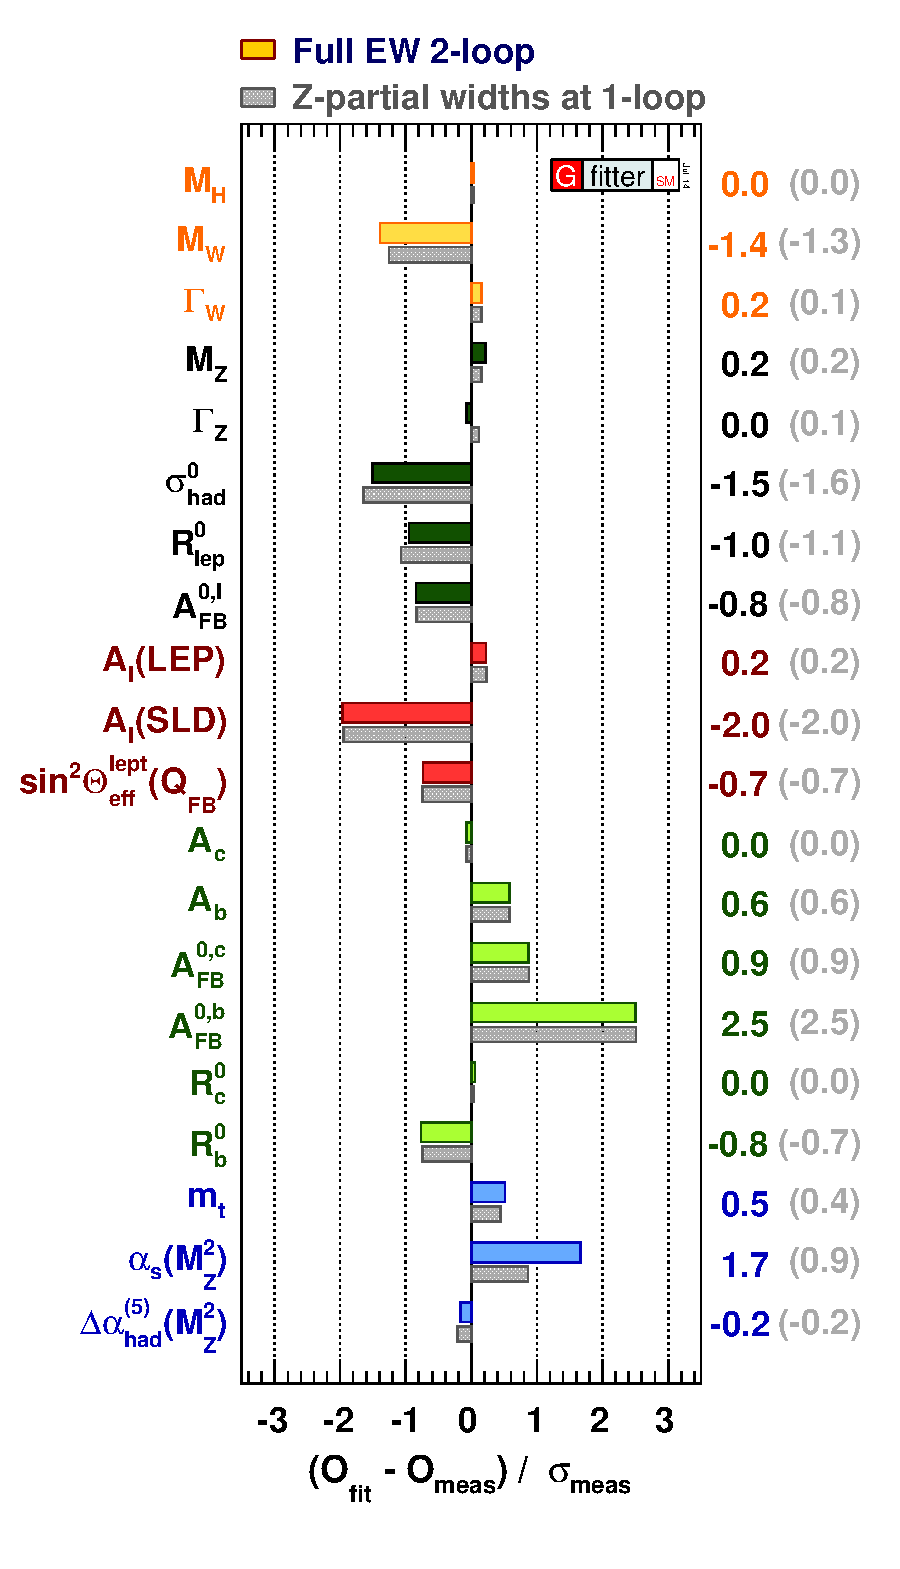
\includegraphics[width=0.45\textwidth]{SM/mesure.eps}
\captionof{figure}{Comparaison des résultats d'ajustement avec les mesures directes de certains paramètres du Modèle Standard.}
\label{mesures}
\end{figure}
\section{Les faiblesses du Modèle Standard}
Le modèle Standard est en accord remarquable avec l'expérience. Cependant, plusieurs problèmes et questions non résolubles amène à considérer le Modèle Standard comme une théorie effective, valable jusqu'à l'échelle du TeV. Une nouvelle physique qui engloberait le Modèle Standard devrait apparaitre à cette échelle d'énergie.

Parmis les principaux problèmes ou faits inexpliqués par le Modèle Standard, on peut citer :
\begin{itemize}[label=$\bullet$]
\item \textbf{Les neutrinos massifs :}\marginpar
{
\centering
\includegraphics[width=\marginparwidth]{SM/kamiokande.jpg}
\captionof{figure}{Intérieur du détecteur Super-Kamiokande.}
\label{kamiokande}
}
\marginpar
{
\centering
\includegraphics[width=\marginparwidth]{SM/chooz.jpg}
\captionof{figure}{Coeur du détecteur Double Chooz.}
\label{chooz}
} Les expérience Super-Kamiokande\ref{kamiokande} et GALLEX portant sur l'observation du flux de neutrinos provenant du Soleil et les expériences Double Chooz\ref{chooz} et K2K pour les flux de neutrinos de sources artificielles terrestres ont mis en évidence l'oscillation des neutrinos entre les saveurs leptoniques. Ces oscillations ne peuvent s'expliquer que si les neutrinos sont massifs et s'il existe des neutrinos droits. Bien que le Modèle Standard considére les neutrinos comme des particules de masse nulle et que de parité gauche, il est facile d'y ajouter un neutrino droit dans chaque famille et les couplages au doublet Higgs correspondant afin de rendre compte de ces faits expérimentaux\footnote{C'est d'ailleurs cette extension du Modèle Standard qui est présenté dans ce chapitre.}. Cependant cela aggrave le problème de la hiérarchie des masses car les masses des particules élémentaires s'étalent sur 10 ordres de grandeur !

\item \textbf{Le nombre de paramètres libres :} Le modèle standard contient 18 paramètres libres : les 3 constantes de couplages, les deux paramètres $\lambda$ et $\mu^2$ du potentiel de Higgs, 9 couplages de Yukawa et les trois angles et une phase pour les quarks dans la matrice CKM ainsi que l'angle associé auwx. Et d'autres encore en ajoutant le fait que les neutrinos soit massif.

\item \textbf{Le nombre de familles :} Le nombre de famille a été expérimentalement obtenu en comparant la section efficace hadronique en fonction de l'énergie du centre de masse expérimentale au prédiction théorique différents nombres de familles de neutrinos de masse négligeable. Actuellement on considère que trois familles\ref{neutrinos}. Cependant le fait que les neutrinos soient massif permet l'existance de plus de trois familles si les neutrinos on une masse supérieur à $m_{Z^{0}}/2$.
\begin{figure}[h!]
\centering
\includegraphics[width=0.35\textwidth]{SM/neutrinos.png}
\captionof{figure}{Mesures de la section efficace de production hadronique près de la résonance en Z. Les courbes indiquent les sections efficaces prédites pour deux,trois et quatres espéces de neutrinos avec les couplages du Modèle Standard et de masses négligeables.}
\label{neutrinos}
\end{figure}

\item \textbf{La baryogénèse :} Le Modèle Standard est incapable d'expliquer l'asymétrie entre la quantité de baryons (matière) et d'anti-baryons (anti-matière) observés dans l'Univers.

\item La gravitation : Le Modèle Standard ne comporte pas l'interaction gravitationnelle. Aucune formulation quantique de la gravitation n'a encore été trouvé. La meilleur théorie gravitationnelle, la relativité générale et malheureusement incompatible avec le Modèle Standard.

\item \textbf{Le problème de naturalité :} En effet, il paraît naturel de considérer une échelle d'énergie ou le Modèle Standard cesse d'être valide. Or, les ordres supérieur de la théorie perturbative ajoutent des corrections radiatives aux masses des différentes particules. En imposant une échelle d'énergie à la validité du Modèle Standard $\Lambda$, un "cut-off", les corrections vont en dépendre. Pour le boson de Higgs et en considérant les diagramme de la figure fig.\cref{corrections} on peut écrire :
\begin{equation}
m_{h}^{2}=m_{0}^{2}-\delta m_{h}^{2}
\end{equation}
avec $m_{0}^{2}$ la masse "nue" du boson, $m_{h}^{2}$ la masse effective et $\delta m_{h}^{2}$ les corrections radiative.
\begin{figure}[h!]
\centering
\includegraphics[width=0.55\textwidth]{SM/corrections.jpg}
\captionof{figure}{Correction radiative du premier ordre pour le boson de Higgs.}
\label{corrections}
\end{figure}
La contribution fermionique est de la forme :
\begin{equation}
\label{eq1}
\delta m_{h}^{2}=-\frac{y_{f}^{2}}{16\pi^{2}}\left(2\Lambda^{2}+6m_{f}\log\left(\frac{\Lambda}{m_{f}}\right)\cdots\right)
\end{equation}
En considérant un cut-off de l'ordre de $\Lambda \sim 10^{16}$GeV il faut donc un accord à $10^{-30}$ entre $m_{0}^{2}$ et $\delta m_{h}^{2}$. Ce problème de hiérarchie, et de réglage fin des paramètres ne semble pas naturel.

\item \textbf{La Matière Noire et l'Énergie Noire} : Des observations cosmologiques ont mis en évidence la présence de matière dite noire car elle n'émet pas et n'interagît pas avec les radiations électromagnétiques. Bien que n'ayant jamais été directement observé, son existence et certaines de ses propriétés peuvent être étudiés par leur effets gravitationnelles sur le mouvement de la matière visible, elle serait  également à l'origine de la formation des galaxies et des amas de galaxies, et de leurs répartition de façon non uniforme dans l'Univers. D'après les observations du satellite Plank\ref{Plank},
la matière que nous connaissons ne compose que 4.9\% du totale mass-énergie de l'Univers. La matière noire quant à elle ne compte que pour 26.8\%. Les 68.3\% restant sont composés d'énergie noire. Cette énergie serait responsable de l'accélération de  l'expansion de l'Univers qui à été mis en évidence en 1998 par les projets Supernova Cosmology Project et High-Z supernovae search team. Ni la matière noire ni l'énergie noire ne sont décrites par le Modèle Standard.
\marginpar
{
\centering
\includegraphics[width=\marginparwidth]{SM/plank.jpg}
\captionof{figure}{Le satellite Plank.}
\label{Plank}
} 

\item \textbf{La non unification des couplages : }Les constantes de couplages $\alpha_{1}$,$\alpha_{1}$ et $\alpha_{3}$ respectivement de l'interaction electromagnétique, faible et forte dépendent de l'échelle d'énergie. Il s'avére que ces trois constantes se rapprochent l'une de l'autre à haute énergie mais ne concourent pas en un seul point (cf.fig\ref{constantes}). Bien que n'étant pas en soit un problème, la convergence vers une valeur unique à haute énergie et nécessaire à une théorie "du tout" qui unifierait ces trois interactions. Le calcul de l'évolution de ces constantes par la méthode de renormalisation n'aboutissant pas à la convergence de ces trois constantes tend à prouver une lacune du Modèle Standard et son caractère effectif.
\begin{figure}[h!]
\centering
\includegraphics[width=0.6\textwidth]{SM/couplageSM.jpg}
\captionof{figure}{Évolution des constantes de couplage en fonction de l'échelle d'énergie dans le cas du Modèle Standard.}
\label{constantes}
\end{figure}
\end{itemize}

\section{Au delà du Modèle Standard}
Afin de résoudre certains de ces problèmes, de nombreux modèles théorique ont été développé, cependant aucun d'entre eux n'est capables de répondre à toutes les questions et combler les lacunes du Modèle Standard. Certaines de ces théorie sont des extensions du à ce modèle, d'autre propose des modèles complètement différents.

La majorité des modèles repose sur les symétries du Modèle Standard et cherche à les étendre : Soit en trouvant d'autres symétries internes (Grand Unified Theorries (GUT)), soit en liant les symétries internes et externes ( supersymétrie (SUSY)) voir même modifier la nature même de l'espace temps en ajoutant des dimensions supplémentaires par exemple.

\subsubsection{Les modèles de grande unification}
Ces modèles s'appuient sur le fait qu'il ait été possible de réunir dans le Modèle Standard trois des quatre interactions que nous connaissons et que leur constantes de couplage se rapprochent l'une de l'autre à haute énergie. Il semble donc logique de vouloir unir ces trois interactions sous une même symétrie. Il n'existerait alors plus qu'un groupe G et qu'une seule constante de couplage. Ces théories doivent bien sûr être renormalisables et leur groupe doit avoir comme sous groupe celui du Modèle Standard $SU(3)\otimes SU(2) \otimes U(1)$. Les groupes $SU(5)$ et $SO(10)$ ont notamment été étudié.

\subsubsection{Modèles à dimensions supplémentaires}
Ces modèles tentent de supprimer la naturalité et la hiérarchie des échelles d'énergies en faisant tendre l'échelle de Planck vers celle de l'interaction faible. Pour cela ils prennent comme hypothèse que l'espace temps contient des dimensions supplémentaires enroulées compacts. L'interaction gravitationnelle évolue donc dans ces dimension supplémentaires.

\subsubsection{La supersymètrie}
La supersymètrie a été introduite par Weiss et Zumino en 1974. Elle consiste à supprimer les divergences quadratiques  en les annulant grâce à l'ajout de termes supplémentaires. Pour cela on associe à chacun des fermions $f_{L}$ et $f_{R}$ un partenaire scalaire $\tilde{f}_{L}$ et $\tilde{f}_{R}$ possédant les mêmes nombres leptoniques et baryoniques. Ces partenaires contribuent donc aux diagramme de correction radiative de la masse du Higgs (cf.fig\ref{corrections}). Les boucles scalaires ont une contribution positive contrairement aux boucles fermioniques, il est ainsi possible de supprimer le terme en $\Lambda^2$ de la formule (\ref{eq1}). La masse du Higgs est varie alors comme le logarithme de l'énergie $\Lambda$. On supprime ainsi le problème du fine-tuning et de la naturalité. Les équations de renormalisation sont également modifiées et il est possible de faire concourir les constantes de couplages en un point. La supersymètrie est donc également un candidat à une théori du "tout". La supersymètrie souffre cependant de certains problèmes, en effet, les particules superpartenaires sont censé être de même masse que les particules élémentaires. Or aucune superparticule n'a encore été detécté expérimentalement. Il faut donc introduire un mécanisme de brisure de la supersymètrie.

Nombres de ces théories postulent l'existence de nouvelles particules ou d'effets qui peuvent être vérifier expérimentalement. Pour pouvoir savoir laquelle de ces théories décrit au mieux la la nature ou contraindre ces modèles, il est nécessaire de construire de nouveaux accélérateurs toujours plus puissant et des détecteurs de plus en plus perfectionnés. 

\chapter{Le Grand collisionneur de hadrons (LHC)}
\renewcommand\chapterillustration{LHC/lhc}
\ThisULCornerWallPaper{1}{\chapterillustration}
\minitoc
\lettrine[lines=4, slope=-0.5em]{C}{e} chapitre décrit le complexe des accélérateurs du CERN\footnote{Organisation Européenne pour le Recherche Nucléaire (Laboratoire européen de physique des particules)} qui permet d'accélérer les particules, afin d'avoir un faisceau de particules avec une énergie suffisante pour être injecté dans le Grand Collisionneur de Hadrons (LHC\footnote{Large Hadron Collider}) et atteindre une énergie finale de $7$ TeV. Cette description bien que succincte est nécessaire car de nombreux résultats obtenus durant cette thèse ont nécessité l'utilisation d'accélérateurs de ce complexe. Une description du LHC est également donnée, car ses performances présentes et futures déterminent les choix technologiques des détecteurs utilisant son faisceau.

\section{Le complexe d'accélérateurs du CERN}

Le complexe d'accélération (\ref{complexe}) du CERN est une série de machines qui délivrent des faisceaux de particules d'énergies de plus en plus élevées. Chaque machine accélère les faisceaux et les injecte dans la machine suivante. Le dernier accélérateur du complexe est le LHC.

Le programme de ce dernier est surtout basé sur des collisions protons-protons. Cependant chaque année, environ un mois est consacré aux collisions d'ions lourds (plomb-plomb) ou (proton-plomb) afin d'étudier notamment le plasma de quarks et gluons, l'une des phases de l'Univers peu après le Big Bang. 

Dans le cas de ces collisions, la chaine d'accélération est constituée du Linear Accelerator 3 (LINAC 3), du Low Energy Ion Ring (LEIR) utilisé pour le stockage des ions et leur refroidissement. La chaine d'accélération est ensuite identique à celle pour les collisions proton-proton.

\begin{minipagewithmarginpars}[h]{\textwidth}
  	\centering
	\includegraphics[scale=0.40]{LHC/complexe.png}
  	\captionof{figure}{Schéma du complexe d'accélération du CERN. La chaine d'injection du LHC est constituée du Linac 2, du Booster, du PS et du SPS}
  	\label{complexe}
  	\par 	
\marginpar
{
	\includegraphics[width=\marginparwidth]{LHC/Bouteille.jpg}
	\label{bouteille}
    	\captionof{figure}{Source des protons du LHC.}
}	
\end{minipagewithmarginpars}

\marginpar
{
	\includegraphics[width=\marginparwidth]{LHC/linac2.jpg}
    \captionof{figure}{Photo du LINAC 2.}
    	\label{linac2}
}

\marginpar
{
	
	\includegraphics[width=\marginparwidth]{LHC/booster.jpg}
    \captionof{figure}{Photo du Booster du Synchrotron à protons.}
    	\label{booster}
}

\marginpar
{
	
	\includegraphics[width=\marginparwidth]{LHC/ps.jpg}
    \captionof{figure}{Photo du PS.}
    	\label{ps}
}

\marginpar
{
	
	\includegraphics[width=\marginparwidth]{LHC/sps.jpg}
    \captionof{figure}{Photo du SPS.}
    	\label{sps}
}
Pour les collisions proton-proton, la source de protons est une bouteille de dihydrogène gazeux (fig. \ref{bouteille}). Les atomes d’hydrogène sont injectés dans le Duoplasmatron Proton IOn Source où il sont chauffés et sont soumis à un champ électrique, qui arrache leurs électrons et les ionise en $H^{+}$ (proton). Les protons extraits sont ensuite envoyés dans l'accélérateur linaire (LINAC 2 (fig. \ref{linac2})) où ils atteignent l'énergie de 50 MeV et sont $5\%$ plus massifs, leur vitesse est alors d'environ $0.3$c où c est la vitesse de la lumière dans le vide (c=$299 792 458$ m/s). Ils passent ensuite dans les 4 anneaux de 157m de circonférence du Booster du Synchrotron à protons (BOOSTER (fig. \ref{booster})) qui les amènent à une énergie de 1.4 GeV avant de les injecter dans l'accélérateur suivant, le Synchrotron à protons (PS (fig. \ref{ps})). Cet accélérateur circulaire de 628 mètres de circonférence, permet aux faisceaux d'atteindre une énergie de 25 GeV, leur vitesse est alors de 0.87c. Il sert aussi à préparer le faisceau en le découpant en série de paquets (bunchs) de particules nécessaires au LHC. Ces bunchs sont ensuite envoyés dans le supersynchrotron à protons (SPS (fig. \ref{sps})) d'une circonférence de 7 km, où l'énergie du faisceau atteint 450 GeV soit une vitesse de 0.99c. Les paquets sont regroupés pour former des trains de paquets avant d'être enfin envoyés dans le Grand Collisionneur de Protons (LHC). L'injection et le guidage de faisceaux d'une telle énergie par des aimants supraconducteurs rapides est une tâche délicate et pourrait détériorer l'accélérateur. Un faisceau de test de faible intensité "pilot beam" est donc injecté afin de mesurer et vérifier les paramètres. Le faisceau de haute énergie est ensuite séparé en deux et injecté dans deux conduits différents, l'un circulant dans un sens et l'autre dans le sens contraire. Ces faisceaux sont ensuite accélérés jusqu'à une énergie de 7 TeV et ne se croisent qu'aux points d'intéractions. À ce stade, les protons on une vitesse de 0.999999991c, soit 299 792 455,3 m/s. Il ne se déplace que 2.7m/s moins vite que la lumière. Afin d'accélérer les protons à une vitesse si proche de la lumière, d'importantes contraintes de pressions et de température sont nécessaires. Un vide poussé est nécessaire à l'intérieur du LHC afin de minimiser les interactions, la pression interne est de l'ordre de $10^{-13}$atm soit 10fois moins que la pression à la surface de la Lune. La présence d'aimants supraconducteurs nécessite un système de distribution cryogénique, qui assure la circulation d'hélium super-fluide est maintient le LHC à une température de $-271,3$\degre C ($1.9$K). Le LHC est donc plus froid que l'Univers (Le fond diffus cosmologique à en effet été évalué par le satellite Plank (cf.fig\ref{Plank}) (2009-2013) à $2,725$K.

\section{Le Large Hadron Collider}
Le LHC est le dernier accélérateur circulaire du complexe d'accélération. Il utilise le tunnel de 27 km de circonférence situé à une centaine de mètres sous terre. Il fût construit pour acceuillir le Grand collisionneur électron-positron (LEP\footnote{Large Electron Positron collider.}), qui fût en service de 1989 à 2000. Le LHC à été mis en service en 2008 et a été construit afin de produire de l'ordre de 600 millions de collisions proton-proton par seconde à une énergie au centre de masse de $\sqrt{s}=14$ TeV. Il est actuellement l'accélérateur de proton-proton le plus puissant du monde, et a permis de mettre en évidence l'existence du boson de Higgs, dernière pièce manquante du Modèle Standard.

Le LHC est un collissioneur de particules non fondamentales (hadrons) à l'inverse de son prédécesseur, le LEP qui utilisé des électrons et des positrons. Lors d'une collission entre hadrons, ceux sont ses constituant élementaires, les quarks et les gluons qui collissionnent entre eux. Ceux-ci possèdent seulement une portion de l'énergie du hadrons qui les contient. L'énergie du centre de masse de cette collision n'est donc pas connue avec précision. Le LHC est donc une machine de découverte de particules plutôt qu'une machine de mesures de précisions comme l'était le LEP, car il permet d'acceder à un large spectre en énergie. Généralement, les mesures de précision sont effectué grâce à des collisionneur utilisant des particules élémentaires ($e^{-}$,$e^{+}$); ils sont dans ce cas souvent linéaire afin d'éviter la perte d'énergie par rayonnement synchroton.

La figure \ref{lhcschema} est une vue schématique du LHC. En vérité le LHC n'est pas parfaitement circulaire, mais est composé de $8$ octants composés d'une section droite de longueur $~5$ km et d'un secteur courbe d'une longueur de $~3$ km (fig. \ref{octants}). Afin de courber les faisceaux 1232 aimants dipolaires de 15 mètres de long sont utilisés et 392 aimants quadripolaires de 5 à 7 mètres servent à concentrer les faisceaux. Les sections droites sont utilisées afin de faire collisionner les deux faisceaux de protons venant en sens inverse l'un de l'autre. Il existe $8$ points potentiels d'interactions (P), mais seulement $4$ sont le siège de collisions et possèdent des détecteurs qui analysent les données issues de ces collisions : le point P1 pour ATLAS\footnote{A Toroidal LHC ApparatuS, détecteur généraliste.}, le point P2 pour ALICE\footnote{A Large Ion Collider Experiment, dédié à l'étude du plasma de quarks et gluons.}, le point P5 pour CMS\footnote{Compact Muon Solenoid, détecteur généraliste.} et le point P8 pour LHCb\footnote{Large Hadron Collider beauty experiment, dédié au quark b.}.

\marginpar
{
	\includegraphics[width=\marginparwidth]{LHC/atlas.png}
    \captionof{figure}{ATLAS.}
    	\label{atlas}
}
\marginpar
{
	\includegraphics[width=\marginparwidth]{LHC/alice.png}
    \captionof{figure}{ALICE.}
    	\label{alice}
}
\marginpar
{
	\includegraphics[width=\marginparwidth]{LHC/cms.png}
    \captionof{figure}{CMS.}
    	\label{cms}
}
\marginpar
{
	
	\includegraphics[width=\marginparwidth]{LHC/lhcb.png}
    \captionof{figure}{LHCb.}
    	\label{lhcb}
}

\begin{minipagewithmarginpars}[h]{\textwidth}
  	\centering
	\includegraphics[scale=0.7]{LHC/CERNMap.jpg}
  	\captionof{figure}{Vue schématique du LHC.}
  	\label{lhcschema}	
\end{minipagewithmarginpars}

\begin{minipagewithmarginpars}[h]{0.95\textwidth}
  	\centering
	\includegraphics[width=0.55\textwidth]{LHC/lhc-schematic.jpg}
  	\captionof{figure}{Vue schématique des octants du LHC ainsi que des positions des principaux détecteurs le long du LHC. Les faisceaux (en bleu et rouge) circulent en sens inverse l'un de l'autre.}
  	\label{octants}	
\end{minipagewithmarginpars}
La réutilisation du tunnel du LEP et l'énergie des faisceau (7 TeV) à obligé l'utilisation d'aimant supraconducteur produsant des champs magnétique de 8.4T. De plus l'utilisation de deux faisceaux de protons voyant en sens inverse et l'espace limité dans le tunnel à amené à la création d'un nouveau type d'aimants où les deux tubes contenant les deux faisceaux sont insérés dans un même cryostat (cf.fig\ref{dipole}).

\begin{minipagewithmarginpars}[h]{0.95\textwidth}
\centering
\includegraphics[width=0.95\textwidth]{LHC/dipole.jpg}
\captionof{figure}{Vue en transversale d'un dipole du LHC.}
\label{dipole}	
\end{minipagewithmarginpars}

\section{Luminosité des faisceaux}
Le nombre d'événement correspondant à un processus donnée que peut produire le LHC peut être exprimé par :
\begin{equation}
N=\int \mathcal{L}(t)\sigma \mathrm dt
\end{equation}
où $\sigma$ est la section efficace du processus considéré ( la probabilité q'un événement produise ce processus ), $t$ la durée de prise de donnée et $\mathcal{L}$ la luminosité instantanée délivré par la machine.

La luminosité est déterminée par les paramètres des faisceaux de protons :
\begin{equation}
\mathcal{L}=\frac{f_{rev}n_{p}N_{}}{4\pi \sigma_{x} \sigma_{y}} F(\phi)
\end{equation}
avec $N_{f}$ le nombre de protons par paquet, $n_{p}$ le nombre de paquets, $f_{rev}$ la fréquence de rotation d'un paquet, $\sigma_{x}$,($\sigma_{y}$) la moyenne quadratique horizontale (verticale) transverse de la taille du faisceau au point d'intéraction et $F(\phi)$ est le facteur de réduction géométrique définit en fonction de l'angle $\phi$ de Piwinski.
\begin{equation}
F(\phi)=\frac{1}{\sqrt{1+\phi^{2}}}
\end{equation}
En considérant des faisceau se croisant dans le plan verticale (cf.fig\ref{collision}), l'angle de Piwinski peut s'écrire :
\begin{equation}
\phi=\frac{\theta_{c}\sigma_{z}}{2\sigma_{y}}
\end{equation}
avec $\theta_{c}$ l'angle de croisement des faisceaux, $\sigma_{z}$ la moyenne quadratique de la longueur d'un paquet.


\begin{minipagewithmarginpars}[h]{0.95\textwidth}
\centering
\includegraphics[width=0.5\textwidth]{LHC/collision.png}
\captionof{figure}{Schéma de colisions de paquets dans le plan transversale.}
\label{collision}	
\end{minipagewithmarginpars}

Il est possible d'exprimer $\sigma_{x}$ et $\sigma_{y}$ en fonction de l'émittance $\epsilon$ et de la fonction $\beta(s)$. L'émittance est l'espace dans l'espace des phase qui contientun certain pourcentage des particules du faisceau ( 95\% pour les collisionneur hadroniques). Elle est supposée constante durant toute la durée du temps de mesure \footnote{d'après le théorème de Liouville} :
\begin{equation}
\sigma_{x}=\sqrt{\epsilon\beta_{x}}
\end{equation}
avec s la postion le long de la trajectoire nominale du faisceau.

La valeur de la fonction $\beta$ au point d'interaction est noté $\beta^{*}$.En considérant de plus que $\sigma_{x}=\sigma_{x}=\sigma$ on peut réécrire $\mathcal{L}$ comme :
\begin{equation}
\mathcal{L}=\frac{f_{rev}\gamma\beta n_{p}N_{p}}{4\epsilon_{n}\beta^{*}\pi} F(\phi)
\end{equation}
où $\epsilon_{n}=\epsilon\gamma\beta$ est l'émittance normalisé, $\gamma$ le facteur de Lorentz $\beta=v/c$.

D'après cette formule on peut remarqué qu'il peut être interéssant de réduire au maximun $\epsilon_{n}$ c'est à dire d'avoir des paquet dont les particules ont la même quantité de mouvement et son proche l'une de l'autre. Il est aussi possible de réduire le facteur de réduction géométrique en utilisant une configuration de faisceau dite en "crabe" (cf.fig\ref{crabe})

\begin{minipagewithmarginpars}[h]{0.95\textwidth}
\centering
\includegraphics[width=0.5\textwidth]{LHC/crab.png}
\captionof{figure}{Schéma de colisions "en crab" de paquets dans le plan transversale.}
\label{crabe}	
\end{minipagewithmarginpars}

La luminosité du faisceau ne reste pas constante tout le long d'un cycle de prise de donnée. La cause principale sont les collisions dans les détecteurs.Le temps de décroissance caractéristique de l'intensité du faisceau par les collisions est :
\begin{equation}
\tau{collisions}=\frac{N_{0}}{L_{0}\sigma_{tot}n}
\end{equation}
avec $N_{0}$ le nombre de protons à l'injection, $L_{0}$ la luminosité initiale,$\sigma_{tot}$ la section efficace totale et $n$ le nombre de point d'interactions des faisceaux.

Les deux autres causes principales de la réduction de la luminosité des faisceaux sont d'une part la perte par interaction entres les particules du faisceaux et le gaz piégé dans les tubes (avec un temps caractéristique $\tau_{gaz}$) ainsi que par diverses perturbations et imperfections ( champ magnétique par exemple ) qui peuvent dévier les particules de la trajectoire nominale du faisceau ($\tau_{imper}$) . 
La décroissance de la luminosité instantanée peut être donné par la formule:
\begin{equation}
\frac{\mathrm \mathcal{L}}{\mathrm t} = L_{0} e^{-\frac{t}{\tau}}
\end{equation}
avec
\begin{equation}
\frac{1}{\tau} = \frac{1}{\tau_{collisions}}+\frac{1}{\tau_{gaz}}+\frac{1}{\tau_{imper}}
\end{equation}

Lorsque l'intensité du faisceau devient trop faible pour une prise de données efficace, les faisceaux sont déviés de leurs trajectoires circulaires et envoyé dans les "dump blocks" (cf.fig\ref{dump})
\marginpar
{
	\includegraphics[width=\marginparwidth]{LHC/dump.png}
    \captionof{figure}{Schéma d'un "dump block".}
    	\label{dump}
}

La luminosité intégré pour les collisions protons-protons délivré par le LHC en 2016 ainsi que celle enregistré par  le détecteur CMS est donné par le graphique suivant :
\begin{minipagewithmarginpars}[h]{0.95\textwidth}
\centering
\includegraphics[width=0.7\textwidth]{LHC/luminosity.png}
    \captionof{figure}{Luminosité intégrée en fonction du jour de l'année 2016 délivrée (bleu) et enregistrée par CMS (orange) pendant les faisceaux stables et pour les collisions pp à 13 TeV d'énergie dans le centre de masse en 2016.}
\end{minipagewithmarginpars}

\chapter{Le détecteur Compact Muon Solenoid (CMS)}
\renewcommand\chapterillustration{CMS/cms.jpeg}
\ThisULCornerWallPaper{1}{\chapterillustration}
\minitoc

\lettrine[lines=4, slope=-0.5em]{C}{e} chapitre décrit le détecteur CMS et les sous-détecteurs qui le compose, suivi d'une discussion sur le système de déclenchement. Il décrit également certaines des mises à niveaux qui se dérouleront durant les \textit{Long Shut Down} LS2 et LS3 afin de se préparer à l'augmentation de la luminosité et de l'empilement qui en découle.

\section{Le détecteur Solénoïde compact à muons (CMS)}
Le détecteur Solénoïde compact à muons abrégé en CMS (pour Compact Muon Solenoid) est avec ATLAS une expérience généraliste qui a comme buts majeurs :

\begin{itemize}[label=$\bullet$]
	\item \textbf{La recherche du boson de Higgs : } Lors de la conception de CMS dans les années 1990, la détection du boson de Higgs à été prise comme référence afin de tester les performances du design du détecteur. Ce but à été réalisé avec la découverte d'une particule compatible avec le boson de Higgs le 4 juillet 2012.
	\item \textbf{Confirmer et préciser les mesures de la physique du Modèle Standard : } Des mesures de précisions dans des domaines tels que la QCD, le couplage électrofaible, et la physique des saveurs pourraient donner des indications d'une physique au-delà du Modèle Standard.
	\item \textbf{La recherche de signes de physique au-delà du Modèle Standard : }CMS permet la recherche de particules supersymétriques ou de nouveaux bosons vecteurs massifs ($Z'$) ou encore la recherche de dimensions supplémentaires par exemple.
	\item \textbf{Étudier les collisions d'ions lourds.}
\end{itemize}

Afin de répondre à ces objectifs, le "Technical Design Report" (TDR) \cite{Bayatian:922757} a fixé le cahier des charges et les caractéristiques essentielles du détecteur CMS, à savoir :
\begin{itemize}[label=$\bullet$]
	\item Une bonne identification des muons et une bonne résolution en impulsion sur une vaste gamme d'impulsion pour la région $|\eta|<2.5$, une bonne résolution en masse pour les dimuons ($\approx 1\%$ à 100GeV/c$^{2}$) et la capacité à déterminer de manière certaine la charge des muons d'impulsion $p<$ 1TeV/c.
	\item Une bonne résolution en impulsion pour les particules chargées ainsi qu'une bonne efficacité de reconstruction dans le trajectographe interne (inner tracker). Un déclenchement et un étiquettage efficace pour les jets venant de quarks $\tau$ et $b$, ce qui requiert un détecteur à pixels proche du point d'interaction.
	\item Une bonne résolution pour l'énergie électromagnétique, et une bonne résolution en masse pour les diphotons et dielectrons  ($\approx 1\%$ à 100GeV/c$^{2}$), une grande couverture géométrique ($|\eta|<2.5$), une mesure de la direction des photons et/ou une localisation correcte du vertex primaire d'interaction ainsi qu'une bon rejet des $\pi_{0}$ et une isolation des photons et letptons efficace à haute luminosité.
	\item une bonne résolution en masse des dijets et une bonne résolution en masse de l'énergie transverse manquante $E_{T}^{miss}$. Ceci requiert un calorimètre hadronique hermétique de très grande couverture géométrique ($|\eta|<5$) et une fine segmentation latérale ($\Delta\eta\times\Delta\phi<0.1\times0.1$)
\end{itemize} 

\subsection{Système de coordonnées conventionnel}
Le système de coordonnées utilisé dans CMS est un repère cartésien $\left(O,\vec{x},\vec{y},\vec{z}\right)$ où $O$ est l'origine du repère et coïncide avec le point nominal d'interaction (IP) qui est le centre du détecteur. Le système de coordonnée est déterminé par l'axe $z$ qui est défini comme étant parallèle et dans la même direction que le faisceau allant dans le sens anti-horaire vue de dessus. L'axe $x$ pointe vers le centre du collisionneur LHC. L'axe $y$ est orthogonal au plan $xz$ et pointe vers le haut. CMS possédant une symétrie cylindrique, le repère $\left(O,\vec{r},\vec{\phi},\vec{z}\right)$ est souvent utilisé. $z$ correspond à la distance entre le plan perpendiculaire à l'axe du faisceau (appelé plan transverse) passant par le point considéré et l'origine $O$ du repère; $\phi$ est mesuré par rapport à l'axe $\vec{x}$ dans le plan $xy$ (angle d'émission par rapport à l'axe du faisceau) et $r=\sqrt{x^2+y^2}$. L'angle polaire $\theta$ est définit par rapport à $z$. Un troisième type de coordonnées, utilisant le fait que les particules produite au LHC sont relativistes, est également utilisé. En décomposant l'impulsion de la particule en une composante transverse et longitudinale $p=p_{T}+p_{L}=\sqrt{p_{x}^{2}+p_{y}^{2}}+p_{z}$ :
\begin{equation}
( E/c)^{2}=(mc)^{2}+p_{T}^{2}+p_{L}^{2}\Longrightarrow ( E/c)^{2}-p_{L}^{2}=(mc)^{2}+p_{T}^{2}\Longrightarrow  \begin{cases}
\left( E/c \right)=\sqrt{\left( mc \right)^{2}+p_{T}^{2}}\cosh(y) \\
p_{L}=\sqrt{\left( mc \right)^{2}+p_{T}^{2}}\sinh(y)
\end{cases}
\end{equation}
%qu'il est possible de réécrire comme :
%\begin{equation}
%\left( E/c \right)=\sqrt{\left( mc \right)^{2}+p_{T}^{2}}\cosh(y), p_{L}=\sqrt{\left( mc \right)^{2}+p_{T}^{2}}\sinh(y)
%\end{equation}
avec $y$ un paramètre appelé rapidité. En remarquant que $p_{l}=p_{z}=p\cos(\theta)$ et en faisant le développement de $E=\sqrt{m^{2}c^{4}+p^{2}c^{2}}$:
\begin{equation}
y=\arctan\left(\frac{p_{l}c}{E}\right)=\frac{1}{2}\log\left(\frac{E+p_{l}c}{E-p_{l}c}\right)=\frac{1}{2}\log\left(\frac{\cos^2 \theta/2+\cdots}{\sin^2 \theta/2+\cdots}\right)\backsimeq-\log\tan\left(\frac{\theta}{2}\right)=\eta
\end{equation}
%en remarquant que $p_{l}=p_{z}=p\cos(\theta)$ et en faisant le développement de $E=\sqrt{m^{2}c^{4}+p^{2}c^{2}}$
%\begin{equation}
%y=\frac{1}{2} \log\left(\frac{E+p_{l}c}{E-p_{l}c}\right)=\frac{1}{2}\log\left(\frac{\cos^2 %\theta/2+m^{2}c^{2}/4p^{2}+\cdots}{\sin^2 %\theta/2+m^{2}c^{2}/4p^{2}+\cdots}\right)\backsimeq-\log\tan\left(\frac{\theta}{2}\right)=\eta
%\end{equation}
$\eta$ est appellé pseudo-rapidité. On utilise donc le repère $\left(O,\vec{r},\vec{\eta},\vec{\phi}\right)$ pour décrire la géométrie de CMS.

\subsection{Description générale de CMS}
Le détécteur CMS se trouve dans une caverne situé au point 5 (P5) du LHC, proche du village de Cessy en France. La construction de CMS s'est effectué en surface et par tranches autonomes afin de réduire le temps et les coûts nécessaires à sa construction.
\marginpar
{
	\centering
	\includegraphics[width=\marginparwidth]{CMS/slice.jpg}
	\captionof{figure}{Descente d'une tranche de CMS.}
	\label{slice}
}
Chaque tranche à ensuite été descendue dans la caverne et assemblée à 100 m sous terre (cf.fig\ref{slice}).
CMS est une détecteur cylindrique de 24m de long et de 14.6 m de diamètre pour une masse de plus de 16000 tonnes (cf.fig\ref{cmsexploded}). Il est composé d'une succession de sous-détecteurs concentriques.

\begin{sidewaysfigure}
	\centering
	\includegraphics[width=0.80\textwidth]{CMS/cms.png}
	\caption{\label{cmsexploded}Vue éclatée du détecteur CMS.}
\end{sidewaysfigure}
\newpage
En partant du centre vers l'extérieur :
\begin{itemize}[label=$\bullet$]
	\item \textbf{Le trajectographe : } C'est le sous-détecteur le plus proche du point d'intéraction. Il permet de reconstruire la trajectoires des particules chargées.
	 \item \textbf{Le calorimètre électromagnétique (ECAL\footnote{Pour Electromagnetic CALorimeter.})}: Il permet de mesurer l'énergie des photons et des électrons.
	 \item \textbf{Le calorimètre hadronique (HCAL\footnote{Pour Hadronic CALorimeter})}: Il permet de mesurer l'énergie des hadrons.
	 \item \textbf{L'aimant supra-conducteur : } Il produit un champ de 3.8T et permet de courber la trajectoire des particules chargées.
	 \item \textbf{Les chambres à muons : } Elles permettent d'identifier, reconstruire la trajectoire et mesurer l'énergie des muons. 
\end{itemize}
Chaque composant de CMS fera l'objet d'une description plus détaillée dans les paragraphes suivants.

\section{Les sous detecteurs de CMS}
\subsection{Le trajectographe}
Le trajectographe de CMS (cf.fig\ref{trajectographe}) est le détecteur le plus proche du faisceau et du point de collision. Le trajectographe est composé de deux sous-détecteurs : le détecteur à pixels et le trajectographe à micro-piste de silicium. Il a pour but de reconstruire les traces des particules chargées issues des collisions grâce à des suites d'impacts enregistrés par les couches du détecteur. La trace reconstruite permet de déterminer la charge et l'impulsion de la particule associée. En effet, une particule de charge $q$ qui se déplace dans un champ magnétique subit une force donné par la formule de Lorentz. La trajectoire de la particule dans le cas d'un champ magnétique d'intensité $B$ est hélicoïdale, de rayon $R_{c}$. Il est ainsi possible dans déduire l'impulsion transverse :
\begin{equation}
p_{T}=qBR_{c}
\end{equation}
En prenant les positions selon r des hits, il est possible d'en déduire l'angle $\theta$, angle entre la trajectoire de la particule est le faisceau et donc de calculer l'impulsion totale:
\begin{equation}
p=\frac{p_{T}}{\sin\theta}
\end{equation}
\begin{figure}[ht!]
	\centering
	\includegraphics[width=0.65\textwidth]{CMS/tracker.png}
	\captionof{figure}{Schéma du trajectographe de CMS. Chaque trait représente un module du détecteur. Les lignes doubles correspondent à des modules mis dos à dos produisant des hits dit stéréo. Le détécteur à pistes est composé de quatre sous-détecteurs : Les tonneaux internes (TIB), les tonneaux externes (TOB), les disques interne (TID) et les bouchons (TEC).}
	\label{trajectographe}
\end{figure}

\subsubsection{Le détecteur à pixels}
Le détecteur à pixels de CMS a récemment été remplacé afin de garder une trajectographie performante à des luminosités au dessus de $2\times10^{34}cm^{-2}s^{-1}$ et avec un empilement de plus de $50$. Ce remplacement a eu lieu du 28 février au 7 mars 2017 durant l'arrêt technique hivernal prolongé (EYETS). Le nouveau détecteur à pixels se compose d'un tonneau constitué de quatre couches de détection (BPIX) à des distances du faisceau $r=3.0$cm, 6.8cm, 10.2cm et 16cm et d'une longueur de 548.8mm et de trois bouchons (FPIX) situé à $\pm$29.1cm,$\pm$39.6cm et $\pm$51.6cm pour une couverture radiale allant de 4.5 à 16.1cm . Une comparaison entre l'ancien détecteur à pixel et le nouveau est donné fig.\ref{pixel}.

	\begin{figure}[ht!]
	\subfloat[Vue oblique-transverse comparant les couche des tonneaux de l'ancien (gauche) et du nouveau détecteur]{\includegraphics[width=.45\linewidth]{CMS/pixel.png}}
	\hfill
	\subfloat[Ancien détecteur à pixel (bas) et nouveaux (haut).]{\includegraphics[width=.45\linewidth]{CMS/pixel2.png}}
	\caption{Comparaison entre le nouveau et l'ancien trajectographe à pixels.}
	\label{pixel}
\end{figure}

L'ajout d'une quatrième couche de détection dans le barrel assure une redondance lors de la reconnaissance de motifs et permet de réduire le taux d'erreur lors d'empilement importants. Il assure également une sécurité au cas où la couche la plus proche du point d'interaction viendrait à se détériorer plus vite que prévu. Cependant, elle augmente le budget matériel du détecteur, il a donc été nécessaire de repenser le support et les services afin d'être plus léger. Un nouveau système de refroidissement au $CO2$ ainsi que la déplacement des système passif (connectique , plaques d'électronique) hors du volume de trajectographie à également été effectué (cf.fig\ref{pixel2}).

\begin{figure}[ht!]
	\centering
	\includegraphics[width=0.80\textwidth]{CMS/pixel3.png}
	\captionof{figure}{Vue explosée du nouveau détecteur à pixels. La figure montre les positions des différentes partitions FPIX et BPIX ainsi que leur cylindres contenant leur service respectifs. Les services nécessaires au détecteur (connectiques, fibre optique, convertisseur DC-DC sont situés à haut $\eta$, hors du volume de trajectographie.)}
	\label{pixel2}
\end{figure}

Ce détecteur contient plus de 97 millions de pixels (79 pour les BPIX et 18 pour les FPIX) mesurant $100\times150\mu m$ de section et $250\mu m$ d'épaisseur. Ces pixels sont regroupés en modules (1184 pour BPIX et 672 pour FPIX) (cf.fig\ref{module}) de 66560 pixels  (8$\times$ 2 ROCs) d'une épaisseur de $75\mu m$ pour la première couche du BPIX et $250\mu m$ pour les reste du BPIX et FPIX.

	\begin{figure}[ht!]
	\centering
	\subfloat[Module pour les couches 2 à 4 des BPIX et des FPIX (gauche) et de la couche 1 de BPIX (droite)]{\includegraphics[width=.46\linewidth]{CMS/module.png}}
	\subfloat[Schéma de l'électronique de lecture d'un module]{\includegraphics[width=.46\linewidth]{CMS/module2.png}}
	\caption{Modules de pixels.}
	\label{module}
\end{figure}
\subsubsection{Le détecteur à pistes}
Le détecteur à pistes mesure 5.5 m de long pour 2.4 m de diamètre pour une aire active de 198m2 et est le plus grand détecteur au silicium jamais construit. Il comporte en tout 15148 modules pour un total de 9.3 millions de pistes lues par 76000 puces électroniques. Il peut être décomposé en quatre sous-détecteurs :

\begin{itemize}[label=$\bullet$]
\item \textbf{Le tonneau interne} Le tonneau interne (TIB) (cf.fig\ref{TIB}) pour  \textit{Tracker Inner Barrel} est composé 2724 modules répartis en quatre couches. Chaque couche se compose de pistes de silicium d'une épaisseur de $320 \mu m$ avec un pas de $80 \mu m$ pour les deux premières couches et de $120\mu m$ pour deux dernières. Elles sont orientées parallèlement au faisceau. Les deux premières couches sont composées de modules dits "stéréos" qui sont la juxtaposition de deux modules collés l'un l'autre avec un angle de $100mrad$ entre les deux. Ce qui permet d'avoir une résolution de $23$ à $34\mu m$ dans le plan transverse et de $230\mu m$ dans le plan longitudinal. Son rayon est compris entre 25 et 52 cm et sa longueur couvre le domaine $|z|<65cm$.

\item \textbf{Les disques internes} (TID) (cf.fig\ref{TID}) pour \textit{Tracker Inner Disk} sont composés de trois disques parallèles qui sont compris dans le domaine $75cm<|z|<110cm$. Chaque disque est composé de trois anneaux concentriques. Les 816 modules sont composés de strips d'une épaisseur de $320\mu m$ orientées radialement pour un pas compris entre $81\mu m$ et $158\mu m$. Comme pour le TIB, les deux premiers modules sont "stéréos".
\marginpar
{
	\centering
	\includegraphics[width=\marginparwidth]{CMS/TOB_TEC.png}
	\captionof{figure}{Différents modules utilisés pour la construction du TOB et du TEC.}
	\label{TOB_TEC}
}
\item \textbf{Le tonneau externe } (TOB) (cf.fig\ref{TOB})pour \textit{Tracker Outer Barrel} entoure les TIB et TID pour couvrir un espace entre 60 et 100cm en rayon et $|z|<110cm$. Il est composé de 5208 modules (cf.fig\ref{TOB_TEC}) de pistes orientées parallèlement au faisceau et de pas compris entre 122 et 183 $\mu m$. Ces modules sont répartis en six couches dont les deux dernieres sont "stéréos". L'épaisseur de ces modules est de $500\mu m$.   

\item \textbf{Les bouchons }(TEC) (cf.fig\ref{TEC}) pour \textit{Tracker End-Cap} sont composés de neuf disques chacun, composée de 4 à 7 anneaux concentriques. Ils couvrent 25-110 cm en rayons et 120-275 cm en $|z|$. Les deux premiers disques ainsi que le cinquième sont "stéréos". Les trois premiers anneaux sont composés de 1256 modules par bouchon (cf.fig\ref{TOB_TEC}) d'épaisseur 320$\mu m$ et de pas inter-pistes compris entre 81 et 158 $\mu m$. Les quatre anneaux suivant, sont composés de 1944 modules par bouchon (cf.fig\ref{TOB_TEC}), d'épaisseur $500\mu m$ de pas inter-strip 113-172 $\mu m$.
\end{itemize}

	\begin{figure}[ht!]
	\centering
	\subfloat[Le TIB.]{\includegraphics[width=.40\linewidth]{CMS/TIB.jpg}\label{TIB}}
	\subfloat[Un TID.]{\includegraphics[width=.40\linewidth]{CMS/TID.jpg}\label{TID}}
	\\
	\subfloat[Le TOB.]{\includegraphics[width=.40\linewidth]{CMS/TOB.jpg}\label{TOB}}
	\subfloat[Un TEC.]{\includegraphics[width=.40\linewidth]{CMS/TEC.jpg}\label{TEC}}
	\caption{Photos des différents composants du détecteur à pistes}
\end{figure}

\newpage
\subsection{Le calorimètre électromagnétique}
Le calorimètre électromagnétique de CMS ou \textit{Electromagnetic CALorimeter} (ECAL), permet de mesurer l'énergie et la direction des particules réagissant principalement à l'interaction électromagnétique. Ce sont surtout les photons et les électrons qui seront détectés; ils perdent leur énergie par des processus radiatifs. La distance caractéristique est donnée par la longueur de radiation $X_{0}$, dépendante du matériau, définie comme le libre parcours moyen pour le processus de radiaction. Des photons de 100 GeV perdent à peu près toute leur énergie dans 20*$X_{0}$.
\begin{figure}[ht!]
	\centering
	\includegraphics[width=0.90\textwidth]{CMS/ECAL.png}
	\captionof{figure}{Schéma du ECAL de CMS.}
	\label{ECAL}
\end{figure}

Le calorimètre électromagnétique est composé de 75848 cristaux (cf.fig\ref{crystaux}) de PbWO4 ($11 m^3$, 92 tonnes)et peut se décomposer en trois sous-structures (cf.fig\ref{ECAL}) :
\begin{itemize}[label=$\bullet$]
	\item \textbf{Le tonneau} ou EB (cf.fig\ref{EB}) pour \textit{Electromagnetic Barrel} contient 61200 cristaux de tungstate de plomb. Le tonneau est divisé en 36 supermodules couvrant chacun la moitié de la longueur du tonneau. Chaque super-module contient 1700 cristaux de 22*22 mm2 et de longueur 230 mm. Les cristaux sont arrangés de manière à former 170-$\eta$ anneaux contenant 360 cristaux chacun. Un cristal couvre environ 1$\degres$ en $\phi$. Le tonneau couvre une zone en pseudorapidité de $|\eta|<1.479$. Les photodiodes à avalanche (cf.fig\ref{APD}) (APD) sont utilisées pour détecter la scintillation.
	\marginpar
	{
		\centering
		\includegraphics[width=\marginparwidth]{CMS/Crystaux.png}
		\captionof{figure}{Un cristal de PbWO4.}
		\label{crystaux}
	}
	
	\marginpar
	{
		\centering
		\includegraphics[width=\marginparwidth]{CMS/APD.png}
		\captionof{figure}{Un groupe de deux APD.}
		\label{APD}
	}
	\marginpar
	{
		\centering
		\includegraphics[width=\marginparwidth]{CMS/dee.jpg}
		\captionof{figure}{Un "Dee".}
		\label{DEE}
	}
	\marginpar
	{
		\centering
		\includegraphics[width=\marginparwidth]{CMS/20SCs.jpg}
		\captionof{figure}{Montage de 20 Super-Cristaux sur un des Dee.}
		\label{SP}
	}
	\marginpar
	{
		\centering
		\includegraphics[width=\marginparwidth]{CMS/VPT.png}
		\captionof{figure}{Une VPT.}
		\label{VPT}
	}
	
	\item \textbf{Les bouchons} (EE) (cf.fig\ref{EE}) pour \textit{Electromagnetic End-cap} sont perpendiculaires au faisceau et ferment le EB. Ils sont situés à 315 cm du point d'interaction et couvrent une section en $\eta$ allant de 1.479 à 3. Chaque bouchon se décompose en deux demi-disques appelés "Dee" (cf.fig\ref{DEE}). Chaque Dee est constitué de 3662 cristaux de 2.86*2.86 cm et de longeur 220 mm regroupés en matrices de 5*5 qu'on appelle Super-Cristaux (cf.fig\ref{SP}). La scintillation est détecté par des phototriode à vide (VPT) (cf.fig\ref{VPT}). Les cristaux de PbWO4 ont une grande densité ($\rho=$8.28g.cm$^{-3}$), une longueur d'interaction $X_{0}$ assez courte de 0.89cm est un petit rayon de molière ($r_{M}$=2.2cm) ainsi qu'une grande vitesse de radiation (80\% dans 25 ns). 
	\item \textbf{L'initiateur de gerbe } (cf.fig\ref{PRESHOWER}), appellé \textit{Preshower} est placé entre le EB et le EE. Il consiste en deux couches de détecteurs de silicium de pas 1.9 mm intercalées entre deux couches en plomb (2$X_{0}$ devant et 1$X_{0}$ derrière la première couche de silicium). Il permet d'améliorer la précision de la mesure de la position de la gerbe électromagnétique et l discrimination $\gamma/\pi_{0}$. Il couvre une région comprise entre 1.653<$|\eta|$<2.6.
\end{itemize}
\begin{figure}[ht!]
	\centering
	\subfloat[Le tonneau du ECAL (EB).]{\includegraphics[width=0.8\linewidth]{CMS/EB.jpg}\label{EB}}
	\\
	\subfloat[Un bouchon du ECAL (EE).]{\includegraphics[width=.40\linewidth]{CMS/EE.jpg}\label{EE}}
	\subfloat[Un des preshower du ECAL.]{\includegraphics[width=.40\linewidth]{CMS/preshower.jpg}\label{PRESHOWER}}
	\caption{Photos des différents composants du Calorimètre électromagnétique.}
\end{figure}
\subsection{Le calorimètre hadronique}
	\marginpar
{
	\centering
	\includegraphics[width=\marginparwidth]{CMS/LAITON.jpg}
	\captionof{figure}{Photo de douilles de la marine russe réutilisées pour la construction du HCAL.}
	\label{LAITON}
}
	\marginpar
{
	\centering
	\includegraphics[width=\marginparwidth]{CMS/SCINTI.png}
	\captionof{figure}{Photo d'une tuile du HO avec des fibres WLS insérées dans les 4 $\sigma$-rainures.}
	\label{SCINTI}
}
\marginpar
{
	\centering
	\includegraphics[width=\marginparwidth]{CMS/MPPC.png}
	\captionof{figure}{Photo d'un MPPC.}
	\label{MPPC}
}
\marginpar
{
	\centering
	\includegraphics[width=\marginparwidth]{CMS/HPD.png}
	\captionof{figure}{Photo d'une HPD.}
	\label{HPD}
}
Le calorimètre hadronique de CMS ou \textit{Hadronic CALorimeter} (HCAL) (cf.fig\ref{HCAL}) permet de mesurer l'énergie et la direction des hadrons issus de l'hadronisation des quarks et gluons produits lors des collisions. Ce détecteur à une grande compacité spatiale et énergétique et est très compact car il se trouve pour une grande partie entre le ECAL et l'aimant supraconducteur. Cette disposition a nécessité de maximiser la quantité d'absorbeur et de minimiser les parties actives du détecteur. L'absorbeur est constitué de laiton (cf.fig\ref{LAITON}) qui possède une faible longueur d'interaction $\lambda_{l}$ et un faible taux de diffusions multiples. Les hadrons perdent majoritairement leur énergie par interaction nucléaire avec l'absorbeur. La plupart des hadrons sont stoppés avec 9$\lambda_{l}$. Le laiton est également non magnétique ce qui est nécessaire vu l'emplacement du calorimètre. Le matériau actif est composé de feuilles de scintillateurs fluorescents (cf.fig\ref{SCINTI}). La scintillation est ensuite récoltée par des fibre optique qui décale la longueur d'onde de la lumière (WLS). Le signal est ensuite lu par des Multi-Pixel Photon Counter (MPPC) (cf.fig\ref{MPPC}) pour le sous-détecteur Hadronic Outward calorimeter et par des photodiodes hybrides (HPD) (cf.fig\ref{HPD}) pour les autres sous-détecteurs.
\begin{figure}[ht!]
	\centering
	\includegraphics[width=0.95\textwidth]{CMS/HCALSCHEME.png}
	\captionof{figure}{Schéma d'un quart d'une coupe du HCAL de CMS.}
	\label{HCAL}
\end{figure}

Le calorimètre hadronique couvre une zone en pseudo-rapidité jusqu'à $|\eta|<5.0$. Il possède plus de 70000 feuilles de scintillateurs. Il est composé de 4 sous-détecteurs subdividsés en tours : 
\begin{itemize}[label=$\bullet$]
	\item \textbf{Le tonneau} HB pour \textit{Hadronic Barrel calorimeter} (cf.fig\ref{HB}) couvre la région en pseudo rapidité $|\eta|<1.3$. Il est constitué de 36 quartiers couvrant 20 degrés en $\phi$ découpé en quatre sous secteurs de 5 degrés en $\phi$ et 16 sous secteurs en $\eta$. Un quartier possède 16 couches qui sont des empilements de scintillateurs de 9mm d'épaisseur pour les couches les plus externes et 3.7mm pour les autres et d'absorbeur (40 mm de fer pour la première couche, 50.5mm de laiton pour les huit suivantes, 56.5 mm de laiton pour les six suivantes et 75 mm de fer pour la dernière). Les tours ont une segmentation de $\Delta\eta\times\Delta\phi=0.087\times0.087$.
	\item \textbf{Les deux bouchons} HE pour \textit{Hadronic End-cap calorimeter} (cf.fig\ref{HE}) couvrent les régions comprises entre $|\eta|>1.3$ et $|\eta|<3.0$. Une zone inclinée à 53 degrés par rapport à l'axe du faisceau et ne pointant pas vers le point d'interaction est laissée libre afin de permettre le passage des câbles et systèmes nécessaires au trajectographe et au calorimètre électromagnétique. Les bouchons sont segmentés en 18 quartiers de 20 degrés en $\phi$ chacun composé de 14 tours en $\eta$. Les tours sont des empilements de scintillateurs de 3.7 mm d'épaisseur et d'une couche d'absorbeur (9mm pour la premiere couche et 7.5mm pour les suivantes). Une tour possède 19 couches de  scintillateurs en tout; les 5 tours couvrant $|\eta|<1.74$ ont une segmentation de $\Delta\eta\times\Delta\phi=0.087\times0.087$ alors que les 8 couvrant $1.74<|\eta|<3.0$ ont des segmentations allant de $\Delta\eta\times\Delta\phi=0.09\times0.174$ à $\Delta\eta\times\Delta\phi=0.35\times0.174$.
	\item \textbf{Le calorimètre externe} HO pour \textit{Hadronic Outward calorimeter} (cf.fig\ref{HO}) est placé à l'extérieur de l'aimant supraconducteur. Il est constitué de couches de scintillateurs de 10 mm d'épaisseur et couvre la région $|\eta|<1.26$. Ce sous-détecteur permet de récupérer l'énergie sortant du HB et assure une longueur d'interaction de plus de 10$\lambda_{l}$. Le HO est composé de 5 anneaux de 2.536m de long selon $z$ 
	numérotés -2,-1,0,+1,+2 et de centre $z=-5.324, 2.686, 0, 2.686 $et$ 5.324m$ respectivement. Le premier anneau est composé de deux couches de scintillateurs de 10 mm d'épaisseur placées en r=3.82 m et 4.07 m. Les autres anneaux ne possèdent qu'une couche de scintillateur placé à r=4.07 m. Chaque anneau est segmenté en 12 secteurs en $\phi$. Et chaque secteur est segmenté en 8, 6 et 5 tuiles de scintillateurs (cf.fig\ref{SCINTI}) pour les anneaux 0, $\pm1$, $\pm2$ respectivement.
	\item \textbf{Les calorimètres très à l'avant} HF pour \textit{Hadronic Forward calorimeter} couvrent une zone en pseudo-rapidité comprise entre $|\eta|>3.0$ et $|\eta|<5.0$ et $12.5<r<130cm$. Ils sont situés à une distance $|z|=11.2m$ et font 1.65m de long. Ils consistent en un absorbeur de fer qui intègre des fibres de quarks résistantes aux radiations qui assurent la collection rapide de la lumière Cherenkov. La moitié de ces fibres font toute la longueur du détecteur (1.65m) alors que d'autres commencent à 22 cm (soit 143 cm de long) du bord placé vers l'intérieur de CMS. Elles sont placées alternativement à une distance de 5 mm l'une de l'autre en $r$  avec segmentation de $\Delta\eta\times\Delta\phi=0.175\times0.175$. Cette différence de longueur permet de séparer les cascades électromagnétiques des cascades hadroniques. La lumière est ensuite collectée par des tubes photo-multiplicateur (PMT). Le HF est composé de 18 secteur de 20 degrés en $\phi$. Chaque secteur comporte 13 anneaux en $\eta$.
\end{itemize}
\begin{figure}[ht!]
\centering
\subfloat[Le tonneau du HCAL (HB).]{\includegraphics[width=.40\linewidth]{CMS/HB.jpg}\label{HB}}
\subfloat[Un bouchon du HCAL (HE).]{\includegraphics[width=.40\linewidth]{CMS/HE.jpg}\label{HE}}
\\
\subfloat[Installation du HO.]{\includegraphics[width=.40\linewidth]{CMS/HO.jpg}\label{HO}}
%http://cms.desy.de/e53612/e155171/e155181/
\subfloat[Un des HF du HCAL.]{\includegraphics[width=.40\linewidth]{CMS/HF.jpg}\label{HF}}
\caption{Photos des différents composants du calorimètre hadronique.}
\end{figure}	
\subsection{L'aimant supraconducteur}
L'aimant supraconducteur de CMS (cf.fig\ref{MAGNET}) est un solénoïde de 5.9 m de diamètre pour 12.9 m de longueur qui a été prévu pour créer un champ magnétique de 4 T à un courant de 19.14 kA. A pleine puissance, il stocke une énergie de 2.7 GJ. Il est composé de 5 bobines en nobium-titane composées de 2168 spires, refroidies à une température de 4.2 K par de l'hélium liquide. Une structure de retour de champ en fer de 11500 t, composée de 5 culasses (cf.fig\ref{CULASSE}) et 2 bouchons, chacun composé de 3 disques, l'entoure et sert de structure de maintien des chambres à muons. L'épaisseur totale du retour est d'environ 1.5 m (l'épaisseur du troisième disque des bouchons et du premier anneau du tonneau est de 30 cm) et les autres disques des bouchons ainsi que les deuxième et troisième anneaux du tonneau font 60 cm. L'épaisseur à été étudiée afin d'être suffisante pour absorber les hadrons qui traverseraient les calorimètres et l'aimant tout en restant assez fin pour éviter les pertes radiatives pour les muons.
\marginpar
{
	\centering
	\includegraphics[width=\marginparwidth]{CMS/CULASSE.jpg}
	\captionof{figure}{Photo d'une Cullasse.}
	\label{CULASSE}
}
\begin{figure}[ht!]
	\centering
	\includegraphics[width=0.50\textwidth]{CMS/MAGNET.png}
	\captionof{figure}{Schéma de l'aimant supra-conducteur de CMS.}
	\label{MAGNET}
\end{figure}
\newpage
La figure \ref{CHAMP} montre une simulation par éléments-finis de la valeur du champ magnétique en fonction de la position.
\begin{figure}[ht!]
	\centering
	\includegraphics[width=0.90\textwidth]{CMS/CHAMP.png}
	\captionof{figure}{Valeur du champ magnétique (gauche) et lignes de champ (droite) selon une coupe longitudinale du détecteur CMS, prédits par la simulation. Pour une valeur du champ central de 3.8 T.}
	\label{CHAMP}
\end{figure}
\subsection{Le spectrographe à muons}

Le spectographe à muons (cf.fig\ref{CMS1},fig\ref{CMS2}) a pour but d'identifier les muons, de mesurer avec précision leur quantité de mouvement et de déclencher sur les événements contenant des muons.
\marginpar
{
	\centering
	\includegraphics[width=\marginparwidth]{CMS/MUON.png}
	\captionof{figure}{Quart d'une coupe dans le plan transverse du détecteur CMS montrant la trajectoire d'un muon (courbe bleue).}
	\label{MUON}
} Les muons ont un très grand pouvoir de pénétration. Il est donc possible d'utiliser à la fois les traces chargées laissées dans le trajectographe et dans des détecteurs placés après l'aimant pour les identifier et les reconstruire de manière précise. Une bonne résolution de la quantité de mouvement des muons et leur bonne identification est obtenue grâce au champ magnétique intense de l'aimant et du retour de champ dans la culasse qui assure une trajectoire avec une double courbure. Cette culasse doit contenir des détecteurs de grande taille afin d'augmenter la probabilité de détection; ils faut donc qu'ils soient peu onéreux et fiables. Il faut également que ces détecteurs ne soient pas atteints par d'autres particules afin d'assurer un signal propre, pour ce faire la distance depuis l'aimant jusqu'à la dernière station du spectrographe et de l'ordre de 16 longueurs de radiation, ce qui évite le bruit de fond hadronique résiduel venant du faisceau.

\begin{sidewaysfigure}
\centering
\includegraphics[width=0.80\textwidth]{CMS/CMSLONG.png}
\captionof{figure}{Coupe longitudinale d'un quart de CMS.}
\label{CMS1}
\end{sidewaysfigure}


\begin{figure}[p]
\centering
\includegraphics[width=0.98\textwidth]{CMS/CMSTRANS.png}
\captionof{figure}{Coupe transversale de la partie centrale CMS.}
\label{CMS2}
\end{figure}

Le spectographe à muons, est composé de 3 sous-détecteurs :
\begin{itemize}[label=$\bullet$]
	\item \textbf{Les chambres à dérive} DT pour \textit{Drift Tube} (cf.fig\ref{DT}) sont présents seulement dans le tonneau ou le flux de muon est faible tout comme le bruit de font des neutrons; Le champ magnétique est également assez faible (~0.4T) et uniforme. Ce détecteur est constitué de 250 chambres inséré dans la culasse de CMS.Il sont disposés en 4 couches selon r à des distances r=4.0,4.9,5.9 et 7.0m. La culasse est composé selon l'axe $z$ de 5 roues numéroté de -2 à 2, chacune comportant 12 (sauf pour MB4 qui en posséde 14) secteurs dans le plan transverse numéroté à partir de $\phi=0$ couvrant 30 degrees. Ce détecteur couvre une zone en pseudo rapidité $\eta<1.2$. Chaque chambre est constituée de 8 couches de tubes (cf.fig\ref{DT1}) mesurant la courbure de la trajectoire des muons selon $\phi$ est 4 couches pour la courbure selon $\eta$. Chaque ensemble de 4couches est appellé super-couche \textit{superlayer}. Les deux super-couche mesurant $\psi$ sont séparé par 20cm d'aluminium en nid d'abeille. Seul les chambre de MB4 ne possede pas de superlayer mesurant $\eta$ bien que la distance entre les deux superlayer restant reste la même.
	\begin{figure}[ht!]
		\centering
		\includegraphics[width=0.50\textwidth]{CMS/DTchamber.png}
		\captionof{figure}{Schéma d'une chambre à dérive.}
		\label{DT1}
	\end{figure}

    Les tubes d'une couche de la chambre sont constitué de 5 électrodes : un fil d'acier inoxydable au centre du tube composant l'anode, 2 pistes servant de cathodes et 2 pistes servant d'électrode et à mettre en forme le champ électrique. Ces deux électrodes améliore l'uniformité du champ à l'intérieur du tube loin du fil et améliore ainsi la résolution spatiale. Le tube est rempli d'un gaz de ArCO2 85/15. Lorsqu'une particule traverse le tube, elle ionise le gaz qui libère des électrons qui sont ensuite accélérer vers l'anode. Une avalanche se crée prêt du fil, ou le champ électrique est intense, ce qui induit un signal sur le fil. Le temps maximal nécessaire à la propagation du signal est de 380ns. 
    
    	\begin{figure}[ht!]
    	\centering
    	\includegraphics[width=0.50\textwidth]{CMS/DTTUBE.png}
    	\captionof{figure}{Schéma d'un tube d'une chambre à dérive.}
    	\label{DT2}
    	\end{figure}
    En estimant le temps d'arrivée des électrons sur l'anode, en supposant le temps d'interaction connu et en ayant trois couche d'un superlayer touché, il est possible d'estimer la position et le temps de la trace. dans un superlayer une resolution de 20mrad en angle 1.5mm en résolution spatial et quelques ns de résolution temporelle sont atteints.
    
    \item \textbf{Les chambres à pistes cathodiques }CSC pour \textit{Cathode Strip Chambers} (cf.fig\ref{CSC}) sont présent dans les bouchons où le flux de muons ainsi que le bruit de fond sont imoportant, le champ magnétique est également non-uniforme. Ces chambre on un temps de réponse très court, une granularité fine et sont presque insensible à la non-uniformité du champ magnétique. Ce détecteur couvre les zones de pseudo-rapidité $0.9<=|\eta|<=2.4$ et consiste en 468 chambres installé dans les bouchons. Chaque bouchons comprends 4 stations nommé ME1 ME2 ME3 et ME4. chaque stations comprends 2 anneaux (sauf ME1 qui en comprends 3) segmenter en 36 chambres couvrant chacunes un angle de 20degree en $\phi$.
    
    Les chambres (cf.fig\ref{CSC2}) sont cosntitués de 6 couches contenant un mélange de gaz (40\% Ar 50\%CO2 qui assure un bon gain et 10\%CF4 afin d'empecher la polymerisation pret des fils.) ainsi q'un plan de pistes de cathode radiale et de fils séparés de 3mm constituant les anodes placés orthogonalement aux pistes (sauf pour les premier anneaux de ME1 ou les fils sont orienté à 26degree afin de compenser la force de Lorentz du au champ magnétique de 4T dans cette zone). Les nombres total de pistes est de 220 000 et plus de 2 millions de fils.
    
    Lorqu'une particule chargée traverse une CSC, elle ionise le gaz. Les electrons sont accéléré vers le fils à anode. Le mouvement de ces charges induit un signal sur les pistes cathode et les fils anode de la chambre. Le temps dérive est beaucoup plus rapide que pous les DT mais la résolution spatiale est faible : 200um dans le plan tansverse et 10mrad dans le plan longitudinal.
    \begin{figure}[ht!]
    	\centering
    	\includegraphics[width=0.50\textwidth]{CMS/CSC2.png}
    	\captionof{figure}{Schéma d'une chambre CSC.}
    	\label{CSC2}
    \end{figure}
    
    
    
	\item \textbf{Les chambres à plaques résistives} RPC pour \textit{Resistive plate Chambers} (cf.fig\ref{RPC}) forment un système très efficace pour trigger sur les muons même à bas $p_{T}$ et sur une zone en pseudo rapidité très large ($|\eta<1.6|$). grâce à sont excellente résolution temporelle (~ns) et compléte les détecteurs CSC et DT dont les résolutions spatiales sont beaucoup plus éleve. Les RPC permettent d'assigner avec une plus grande précision le bon temps de croisement de faisceau pour les muons. Elles sont présentes à la fois dans le tonneaux et les bouchons. Dans le tonneau 480 sont réparti en 6 couches, 2 pour MB1 et MB2 et 1 pour MB3 et MB4. La redondance en MB1 et MB2 permet  de trigger sur les muons de bas $p_{T}$ qui pourrait êttre arrêtés avant d'atteindre MB3. Pour les bouchons, les 432 chambres sont répartis en trois disque noté RE1 RE2 RE3 pour chaque bouchon. Chaque disque est composés de 3 anneaux RE*/1 RE*/2 RE*/3 avec * représentant le numéro du disque. Seul les anneaux 2 et 3 sont instrumentés. Chaque anneaux est ségmenté en 18 chambres couvrant $\phi=20$.
	
	Les RPC sont des chambres à double gap (cf.fig\ref{RPC2}) qui opèrent en mode avalanche afin de fonctionner même à haut rate de particules $~qq centaine de Hz/cm2$. Un gap est constitué de deux plates de bakélite qui servent  dans lequel circule un gaz. Des pistes de lectures sont inséré entre les deux gaps. Le système des RPC dans CMS ainsi que le fonctionnement d'unr RPC est expliqué dans le prochain chapitre.
	  \begin{figure}[ht!]
		\centering
		\includegraphics[width=0.60\textwidth]{CMS/RPC2.jpg}
		\captionof{figure}{Schéma en vue éclaté d'un gap d'une RPC et des pistes de lecture.}
		\label{RPC2}
	\end{figure}
	
	
\end{itemize}
    \begin{figure}[ht!]
	\centering
	\subfloat[Photo d'une cassette contenant une chambre DT et RPC.]{\includegraphics[width=0.40\linewidth]{CMS/DT.jpg}\label{DT}}
	\subfloat[Photo d'une chambre CSC.]{\includegraphics[width=.40\linewidth]{CMS/CSC.jpg}\label{CSC}}
	\\
	\subfloat[Photo d'une chambre RPC.]{\includegraphics[width=.40\linewidth]{CMS/RPC.jpg}\label{RPC}}
	\caption{Photos des différents composants du spectrographe à muons.}
\end{figure}

\section{Le système de déclenchement et d'acquisition de données}
Chaque types de particules lors de sont passage dans CMS va créer des types de traces particulières qui vont être enregistrer sous forme électronique par les sous-détecteur le composant.La figure \ref{particules} montre une vue schématique des traces laissé par différents types de particules dans les sous-détecteurs de CMS.

	  \begin{figure}[ht!]
	\centering
	\includegraphics[width=0.56\textwidth]{CMS/particles.png}
	\captionof{figure}{Schéma des traces laissées par différents types de particules dans les sous détecteurs de CMS.}
	\label{particules}
\end{figure}

Les faisceaux ont une fréquence de croisement de 40MHz, chaque événement créer lors de ces collision ont une taille de l'ordre du Méga-octets. Le flux de donnée est bien trop important pour être stocké (~40TB/s). Le flux de données doit donc être réduit, il est donc nécessaire de rejeter des événements afin d'obtenir une fréquence d'acquisition de l'ordre de 300Hz tout en continuant d'enregistrer les événements intéressants pour la physique. Cette étape est réaliser par le système de déclenchement ou \textit{trigger}. La réduction d'un facteur $10^{5}$ de l'acquisition des données est impossible à réaliser en une seule fois, le trigger est donc constituer de deux étapes appelées \textit{Level-1 Trigger} (L1) qui réduit le flux d'événement à 100kHz et \textit{High-Level Trigger} (HLT) qui réduit ensuite ce flux à 300Hz.

\subsection{Le déclenchement de niveau I (L1)}
Le trigger de niveau I (L1) (cf.fig\cref*{L1}) opére à la fréquence de collision des faisceaux (40MHz). L'électronique des détecteurs lisent est stockent les  signaux électriques et les stockent dans une mémoire tampon de 128 événement de collision soit 3.2$\mu s$. Le système de déclenchement possède donc 3.2$\mu s$ pour  décider s'il doit envoyer les données au déclenchement de haut niveau HLT. Chaque 25ns, un nouvel événement rentre dans la mémoire tampon et la décision de garder ou non l'événement arrivé 3.2$\mu s$ plus tôt est prise. Ces 3.2$\mu s$ correspondent à l'envois des données depuis l'électronique des calorimètres et du spectrographe à muons vers la caverne de services qui contient les processeurs gérant la prise de décision, le retour d'un signal pour le rejet ou l'acceptation de l'événement, le délai de synchronisation entre les parties du détecteur ainsi que le tempos de prise de décision. ($\sim1\mu s$). 

	  \begin{figure}[ht!]
	\centering
	\includegraphics[width=0.70\textwidth]{CMS/L1.png}
	\captionof{figure}{Schéma du L1.}
	\label{L1}
\end{figure}

Chacun des trois sous-détecteur du spectrographe à muons utilise sont propre trigger. Les DT et CSC ont créent des segments de traces. Ces segments sont conservé que s'il pointent vers le point d'interaction. Deux (trois) traces par DT(CSC) sont envoyé au Drift Tube Track Finder (DTTF) (Cathode Strip Chamber Track Finder (CSCTF)) qui cherchent des correspondance entre les traces et assigne un niveau de qualité  au valeur $\eta$ $\phi$ à la charge et à la quantité de mouvement trouvé par ces correspondance et envoie 4 candidat muons au Global Muon Trigger (GMT). Pour le RPC, la sélection est basé sur une coïncidence spatial est temporelle entre les différentes couches. Le Pattern Comparator compare les signaux venant des 4 stations à des patron prédéfini afin de trouver les candidats muons et 8 d'entre eux (4 pour les bouchon 4 pour le tonneau) sont envoyé au GMT. Le GMT reçoit tous ces candidats et combinent ceux trouver dans plusieurs sous-detecteurs. Il assigne ensuite un niveau de qualité à ces nouveau candidats et envois les 4 meilleurs d'enre eux au Global Trigger (GT).

Pour les calorimètre, ils sont réunis en tours de déclenchement qui correspondent aux supercrystaux pour le ECAL. Un candidat est trouvé pour chaque tour du ECAL et HCAL.Le Trigger Primitive Generator est responsable de sommer les énergies venant des différents composant des tours.  Le Regional Calorimeter Trigger (RCT) reçoit les candidats du ECAL et HCAL qui sont répartit en 18 crates qui couvre la moitié des détecteur en $z$ et 40 degree en $\phi$ et fournissent au Global Calorimeter Trigger chacun 4 candidats $e/\gamma$ isolée et 4 candidats non-isolés. Le GCT fournit des informations sur l'isolation et la compatibilité avec des particules d'ionisation minimale au système trigger des muons et classe les candidats $e/\gamma$ par niveau de qualité et envoi les 4 meilleurs isolés et 4 non-isolé au GT. Le GT possèdent également des informations sur les jets, l'énergie transverse totale etc.

La décison finale est faite par le Gloabl Trigger à partir de conditions programmables demandant la présence d'objects ou d'énergie en quantité ou valeurs prédéfinies. Ces conditions forment un chemein de déclenchement. Le Gloabl Trigger permet de programmer et de tester jusqu'à 128 chemins en parallèle. 

\subsection{Le déclenchement de haut niveau (HLT)}
Si l'événement est sélectionné par le L1, il est envoyé au déclenchement de haut niveau (HLT) et les données sont transmises à une ferme de calcul de plusieurs milliers d'ordinateurs  dont chaque processeur exécute le même code de déclenchement (\textit{HLT Menu}) exécuter séquentiellement afin de réduire le temps nécessaire à l'élimination d'un événement et d'améliorer le temps de décision qui doit être de l'ordre de 100ms par événement. Il permet de passer à un flux de donnée de 300Hz. Durant cette phase, les données dui tracker sont utilisés contrairement au L1.

\section{Mises à niveaux et amélioration de CMS}
Le détecteur CMS à déjà subit de nombreuse améliorations depuis le début de sa mise en service (SiPM dans le HO, nouveau trajectographe à pixels...). Cependant, la mise à niveau du LHC vers le HL-HLC prévoit de multiplier la luminosité par $10$, ce qui représente un challenge pour CMS qui doit se mettre à niveau pendant les arrêt LS2 et LS3 afin de pouvoir s'adapter à cette luminosité et au pile-up supplémentaire que cela va engendrer (~140-200 de pile-up). Parmi les mises à niveaux programmées citons \cite{Collaboration:1355706} \cite{Contardo:2020886} :
\begin{itemize}[label=$\bullet$]
	\item Le remplacement des HPD dans les sous-détecteurs HB,HE du calorimètre hadronique pendant le LS2 par des SiPM (comme présent actuellement dans le HO).
	\item Le remplacement complet du trajectographe durant LS3 (cf.fig\ref{tracker2}). La granularité doit être multiplié par 4 afin de gardé une bonne performance de reconstruction malgré l'augmentation du pile-up. Pour cela, les pistes du trajectographe à piste seront raccourcis et le détecteur sera également plus léger afin d'obtenir une meilleur résolution en $p_{T}$ et une conversion des $\gamma$ plus faible. Le trajectographe à pixels aura des pixels et des senseurs plus petit afin d'améliorer la résolution du paramètre d'impact et une meilleur séparation des traces.Plus de 10 disques additionnel dans chaque bouchon seront installé afin de couvrir une zone en rapidité jusqu'à $|\eta|=4$.
	\begin{figure}[ht!]
		\centering
		\includegraphics[width=0.85\textwidth]{CMS/tracker2.png}
		\captionof{figure}{Schéma d'un quart du tracker prévu pour la mise à niveau de CMS.}
		\label{tracker2}
	\end{figure}
	\item Les bouchons des calorimètres devront être remplacés par des calorimètre de haute granularité \textit{High Granularity Calorimeter} (HGC) d'une profondeur totale de ~ 10$\lambda$ qui fourniront des images tridimensionnelles détaillées des gerbes. La section électromagnétique est composée d'une trentaine de couches de tungstène et de plaques de cuivre intercalées avec des capteurs de silicium comme matière active. Les capteurs auront des aires variables inférieures à ~ 1,0 cm2. La section électromagnétique fait environs 25X0 et une longueur d'interaction ($\lambda$). La partie hadronique possède 12 plaques de laiton et de cuivre intercalés avec des capteurs de silicium d'une longueur représentant de 3,5$\lambda$ ce qui couvre la majorité d'une gerbe hadronique. Il est suivi d'un "calorimètre hadronique à l'arrière" de conception similaire à l'actuel HE ( des plaques en laiton intercalé avec des carreaux scintillants en plastique lus avec des fibres optiques à décalage de longueur d'ondes). La conception de ce calorimètre à grande granularité s'appuie sur les concepts du ILC / CALICE [21] pour la mesure 3D des gerbes.
	\item le temps de latence du L1 sera augmenté jusqu'à 12.5$\mu s$ ce qui permettra de au système de reconstruction et de d'identification des traces venant des calorimètres et du spectrographe à muons. Pour cela l'électronique de certains sous-détecteurs déjà existent devront être mise à niveau. La fréquence des données en sortie est estimé à 5000Hz(7000Hz) avec 140(200) de pile-up. Le trigger L1 aura également les informations des traces fournit par le trajectographe pour des traces avec $p_{T}\geqq2	Gev$. Ce qui permettra un meilleur pouvoir de rejet du bruit de fond dès le début de la sélection des événements. Un tout nouveau L1 pour les calorimètres et le spectrographe à muons sera également mis en service(cf.fig\ref{L1_2}).
	\begin{figure}[ht!]
		\centering
		\includegraphics[width=0.60\textwidth]{CMS/L1_2.png}
		\captionof{figure}{Schéma du nouveau L1 pour la partie calorimètre et muons.}
		\label{L1_2}
	\end{figure}
\item Le trajectographe à muons dans le bouchon ne possède que des CSC dans la zone $1.6<\eta<2.4$ actuellement. C'est la seule région du trajectographe qui ne possède pas de RPC afin d'assurer une redondance malgré le fait qu'il s'agissent d'une région dont la résolution de la quantité de mouvement est moins bonne et dont le bruit de fond et important. Afin d'améliorer le L1 dans cette région il est proposé d'instrumenter cette zone avec des chambres de nouvelles technologies. Il est donc prévu d'utiliser des Gas Electron Multiplier (GEM) dans les station ME1 et ME2 qui présente de bonne résolution spatiale et résiste au champ magnétique important présent dans ces zones.Elles permettrons d'améliorer la résolution en quantité de mouvement et d'améliorer la correspondance avec les traces dans le Global Muon Trigger. Pour les deux derniere zone ME3 et ME4, des RPC de meilleur granularité et de bonne résolution temporelle seront utilisées ain de réduire le bruit de fond.  De plus, une nouvelle station ME0 de GEM sera inséré dans l'espace libéré par les nouveaux bouchons de CMS, ce qui augmentera la couverture de détection des muon jusqu'à $\eta\approx3$ (cf.fig\ref{end}). 
	\begin{figure}[ht!]
	\centering
	\includegraphics[width=0.60\textwidth]{CMS/endcap.png}
	\captionof{figure}{Schéma d'un quart du détecteur CMS montrant les différentes technologie qui seront instrumentées dans les bouchons.}
	\label{end}
\end{figure}
\end{itemize}
Ce dernier point et plus particulièrement la caractérisation de détecteurs à plaques résistives de verres de basse résistivité est l'objet de cette thèse et sera développé dans les chapitres suivants. 
\chapter{Les Chambres à plaques résistives de CMS}
\renewcommand\chapterillustration{RPC/rpc}
\ThisULCornerWallPaper{1}{\chapterillustration}
\minitoc

\lettrine[lines=4, slope=-0.5em]{D}{ans} ce chapitre, une description générale des chambres à plaques résistives (RPC) ainsi qu'une description détaillée des chambres RPC utilisées dans CMS et de leurs électroniques. Une description des mises à niveaux se rapportant à ces détecteurs, notamment dans les bouchons sera également présentée.

\section{Les chambres à plaques résistives (RPC)}

 \marginpar
{
	\centering
	\includegraphics[width=\marginparwidth]{RPC/Geiger.png}
	\captionof{figure}{Photo d'un des premiers tubes Geiger-Müller fabriqué en 1932 par Hans Geiger pour une utilisation en laboratoire.}
	\label{Geiger}
}
Les RPC pour \textit{Resistive Plate Chambers} font partie d'une famille de détecteurs appelé détecteurs gazeux. Ces détecteurs ont joué un rôle dès le début de la Physique des Hautes Énergies dans la détection de nouvelles particules. Depuis le premier détecteur gazeux, le compteur proportionnel à un seul fil \textit{Single-wire proportional counter} inventé par Rutherford et Geiger, puis le compteur Geiger-Müller (cf.fig~\ref{Geiger}) présenté en 1928, les détecteurs gazeux n'ont cessé de se perfectionner et de devenir plus rapide et efficaces. Ils permettent de couvrir de grandes surfaces de détections à des coûts très modestes.

\subsection{Les détecteurs gazeux}
Les détecteurs gazeux reposent tous sur le même principe simple. Lorsqu'une particule traverse un gaz, elle l'ionise. Les ions et électrons créés lors de cette ionisation peuvent être accélérés grâce à un champ électrique. En choisissant judicieusement l'intensité du champ électrique, c'est à dire en appliquant une tension aux bornes des électrodes, les électrons peuvent gagner assez d'énergie pour ioniser le gaz à leur tour (seconde ionisation) et commencer une multiplication de charge. Le nombre de charges libérées détermine le mode de fonctionnement du détecteur. Le gaz est également un élément important du détecteur et a un rôle important sur le mode de fonctionnement de celui-ci. Le déplacement des charges à l'intérieur du gaz induit un déplacement de charges sur les électrodes, et crée un signal qui peut être récupéré par une électronique et donner une information sur le temps et la position de la trajectoire de la particule incidente. Ces charges peuvent donner lieu à un mode dit "streamer" voire donner lieu à la création d'étincelles entre l'anode et la cathode. La figure \ref{mult} montre le facteur d'amplification, ou le gain du gaz en fonction du voltage appliqué. 

\begin{figure}[ht!]
	\centering
	\includegraphics[width=0.95\textwidth]{RPC/gasgain.png}
	\captionof{figure}{Évolution typique de gain du gaz en fonction du voltage appliqué (en échelle arbitraire).}
	\label{mult}
\end{figure}

Six régions peuvent être définies :

\begin{itemize}
	\item \textbf{I} Les paires d'électrons-ions primaires se recombinent avant d'avoir été toutes récoltées.
	\item \textbf{II} Les charges dues à l'ionisation primaire sont entièrement récoltées sur les électrodes. Le facteur d'amplification reste constant même si le voltage est augmenté.
	\item \textbf{III} Les charges produites par l'avalanche sont proportionnelles aux charges produites lors de la première ionisation. Les charges collectées augmentent fortement avec la tension appliquée.
	\item \textbf{IV} Cette région est la limite de proportionnalité, l'avalanche se transforme en streamer, un plasma d'ions et d'électrons.
	\item \textbf{V} Les streamers connectent les électrodes et produisent des étincelles visibles. Les compteurs Geiger-Müller et les chambres à étincelles fonctionnent dans ce mode.
	\item \textbf{VI} Des décharges électrique se produisent même sans le passage de particules pour ioniser le gaz. Ce mode peut détruire le détecteur.
\end{itemize}

Les détecteurs gazeux à fils ont une résolution temporelle de l'ordre de la centaine de nanoseconde. Cela est dû au champ électrique en $\frac{1}{r}$, qui fait que la zone d'amplification se situe proche du fil et les électrons doivent atteindre cette zone avant d'être amplifiés et de démarrer l'avalanche.

En utilisant un champ électrique uniforme et important, une meilleure résolution temporelle est atteignable.

Le premier détecteur gazeux utilisant cette méthode est le compteur à étincelle "Spark Counter" développé dans les années 1948, un détecteur qui présente une géométrie plane. Il est généralement constitué de deux électrodes métalliques entre lesquelles est présent un gaz. Le passage d'une particule ionise ce gaz et crée une avalanche qui rentre à un certain moment en mode streamer. Un plasma se crée entre les deux électrodes, les électrodes se déchargent et amènent à la création d'une étincelle. Ce type de détecteur présente un signal qui ne nécessite pas d'amplification, cependant le temps nécessaire à la recharge des électrodes est de l'ordre de quelques millisecondes. De plus la surface du détecteur ne doit pas être trop grande ($\sim$\SI{10}{\square\centi\meter}) afin de ne pas détruire les électrodes lors des décharges.

Afin de résoudre ces problèmes, les électrodes métalliques peuvent être remplacées par des plaques de matériaux de haute résistivité (\SIrange{10e9}{10e10}{\ohm\centi\meter}) afin de limiter l'aire de décharge des électrodes autour du signal. Un mélange de gaz absorbant les photons permet d'éviter le mode streamer. Ce qui permet le fonctionnement du détecteur à des flux de particules plus important. Le champs électrique baissant localement du fait de la recharge plus lente des électrodes, le développement d'avalanches successives au même endroit est limité tout en laissant le détecteur opérationnel hors de cette zone.
\vspace{-0.3cm}
\subsubsection{Naissance des RPC}
\vspace{-0.3cm}
En 1981 R.Santonico et R.Cardarelli développent les Resistive Plate Chamber (RPC) \cite{Santonico:1981sc} \cite{CARDARELLI198820}. Ce détecteur utilise un matériau peu coûteux, très utilisé et de haute résistivité ($\sim$\SI{e10}{\ohm\centi\meter}), le High Pressure Laminate (HPL) fait de mélamine ou un type de résine phénol-formaldéhyde (anhydrure de polyoxybenzylméthylèneglycol ou Bakélite (cf.fig~\ref{bakelite})). 
\marginpar
{
	\centering
	\includegraphics[width=\marginparwidth]{RPC/bakelite.png}
	\captionof{figure}{Structure de la Bakélite.}
	\label{bakelite}
}
Plusieurs configuration pour les RPC sont possibles, mais l'une des plus simples est donnée par la figure \ref{RPCscheme}.

\begin{figure}[th!]
	\centering
	\includegraphics[width=0.98\textwidth]{RPC/scheme_first.png}
	\captionof{figure}{Schéma d'une RPC typique.}
	\label{RPCscheme}
\end{figure}
\vspace{-0.1cm}
Une couche de gaz est comprise entre deux plaques d'électrodes résistives. Ces plaques sont peintes avec du graphite qui est utilisé pour distribuer la haute tension sur les électrodes. L'électronique est isolée de la chambre par un isolant fin, de type feuille de poly(téréphtalate d'éthylène) (Mylar). L'électronique peut être placée de chaque coté de la chambre et peut être constituée de carreaux ou de lamelles etc.

Un modèle électrique simplifié d'un RPC peut être obtenu (cf.ref~\ref{RPCscheme}). En notant, $C_{b}$ la capacité de la bakélite, $R_{b}$ sa résistance et $C_{g}$ la capacité du gaz.

La résistance de la bakélite est donnée par :
\begin{equation}
R_b=\frac{\rho d}{S}
\end{equation}
avec $\rho$ la résistivité de la bakélite, $d$ l'épaisseur de l'électrode et $S$ sa surface.

La capacité de la bakélite est donnée quant à elle par :
\begin{equation}
C_{b}=\epsilon_0\epsilon_r\frac{S}{d}
\end{equation} 
avec $\epsilon_0$ la permittivité du vide et $\epsilon_r$ la permittivité relative de la Bakélite.

Le temps de décharge d'une électrode de telle résistivitéet capacité recevant une charge $Q_{0}$ est donné par :
\begin{equation}
Q(t)=Q_{0}e^{\frac{-t}{R_bC_b}}=Q_{0}e^{\frac{-t}{\rho\epsilon_{0}\epsilon_{r}}}=Q_{0}e^{\frac{-t}{\tau}}
\end{equation}
Les charges présentes sur les électrodes réduisent la haute tension appliquée et donc le champ électrique à l'endroit des charges. Le détecteur devient inefficace pour cette période de temps $\tau$ à l'endroit du dépôt des charges tout en restant efficace ailleurs. Pour le cas de la bakélite $\rho\simeq\SI{10e10}{\ohm\centi\meter}$ le temps de relaxation est de l'ordre de \SI{10}{\micro\second}. Grâce à l'utilisation de matériaux de haute résistivité, l'utilisation de chambres de grande taille était désormais possible.


Depuis, ces détecteurs de construction simple et robuste ont été utilisés dans de nombreuses expériences : ATLAS \cite{ATLAS}, BaBar \cite{Boutigny:1995ib} (cf.fig~\ref{babar}), BELLE \cite{ABASHIAN2002117} (cf.fig~\ref{belle}),  Oscillation Project with Emulsion-tRacking Apparatus (OPERA) \cite{1748-0221-9-10-C10003} (cf.fig~\ref{opera}) etc. Différentes solutions technologiques ont été développées selon les besoins des différentes expériences.

\marginpar
{
	\centering
	\includegraphics[width=\marginparwidth]{RPC/babar.png}
	\captionof{figure}{Schéma de l'expérience BaBar.}
	\label{babar}
}

\marginpar
{
	\centering
	\includegraphics[width=\marginparwidth]{RPC/belle.png}
	\captionof{figure}{Schéma de l'expérience BELLE.}
	\label{belle}
}

\marginpar
{
	\centering
	\includegraphics[width=\marginparwidth]{RPC/OPERA.jpg}
	\captionof{figure}{Photo du détecteur OPERA.}
	\label{opera}
}

\subsection{Principes de fonctionnement d'une RPC}
Le principe d'une RPC repose sur l'ionisation d'un gaz. Lorsqu'une particule relativiste traverse le gaz d'une RPC, elle interagit avec les molécules de gaz principalement par interaction électromagnétique. La perte d'énergie moyenne par ionisation et excitation d'une particule relativiste massive ($m>m_{e}$) due à des électrons libres supposés au repos est donnée par la formule de Bethe-Bloch (cd.fig\ref{Bethe-Block})
\begin{equation}
-\left<\frac{1}{\rho}\frac{\dd E}{\dd x}\right>=\frac{e^{4}}{4\pi \epsilon_{0}^{2}m_{e}c^{2}}z^{2}N_{A}\frac{Z}{A}\frac{1}{\beta^{2}}\left[\frac{1}{2}\ln\frac{2m_{e}c^{2}\beta^{2}\gamma^{2}E_{max}}{I^{2}}-\beta^{2}-\frac{\delta(\beta\gamma)}{2}\right]
\end{equation}
avec :

\begin{itemize}[label=$\bullet$]
	\item $\rho$ la densité du matériau,
	\item $e$ la charge de l'électron,
	\item $\epsilon_{0}$ la permittivité du vide,
	\item $c$ la vitesse de la lumière dans le vide,
	\item $z$ la charge de la particule incidente,
	\item $N_{A}$ le nombre d'Avogadro,
	\item $Z$ le numéro atomique du matériau,
	\item $A$ le nombre de masse du matériau,
	\item $\beta=\frac{v}{c}$ la vitesse de la particule incidente en unité de $c$,
	\item $\gamma=\frac{1}{\sqrt{1-\beta^{2}}}$
	\item $I$ est l'énergie d'excitation moyenne et
	\item $E_{max}$ est l'énergie maximale transférée lors d'une collision d'une particule de masse $m$ et de quantité de mouvement $p$,
	\begin{equation}
	E_{max}=\frac{2m_{e}p^{2}}{m^2+2\gamma m_{e}m+m_{e}^2}
	\end{equation}
\end{itemize}

\begin{minipagewithmarginpars}[h]{0.95\textwidth}
	\centering
	\includegraphics[width=0.70\textwidth]{RPC/Bethe-Bloch.eps}
	\captionof{figure}{Perte d'énergie moyenne $-\left<\frac{\dd E}{\dd x}\right>$ pour des anti-muons dans du cuivre en fonction de $\beta\gamma=\frac{p}{Mc}$ sur neuf ordres de grandeurs en quantité de mouvement (12 ordres de grandeurs en énergie cinétique)\cite{Olive:2016xmw}.}
	\label{Bethe-Block}
\end{minipagewithmarginpars}

\marginpar
{
	\centering
	\includegraphics[width=\marginparwidth]{RPC/Photon.png}
	\captionof{figure}{Émission d'un photon lors de la désexcitation d'un atome.}
	\label{photon}
}
\marginpar
{
	\centering
	\includegraphics[width=\marginparwidth]{RPC/Auger.png}
	\captionof{figure}{Éjection d'un électron Auger.}
	\label{Auger}
}
\marginpar
{
	\centering
	\includegraphics[width=\marginparwidth]{RPC/Penning.png}
	\captionof{figure}{Ionisation Penning.}
	\label{Penning}
}
\marginpar
{
	\centering
	\includegraphics[width=\marginparwidth]{RPC/Brem.png}
	\captionof{figure}{Bremsstrahlung produit par un électron dévié par le champ électrique d'un noyau.}
	\label{Brem}
}

Si un atome ou une molécule du gaz est ionisé par la collision inélastique de la particule incidente, des électrons sont éjectés de l'atome près du point de collision. En revanche, si l'atome n'est pas ionisé mais excité, l'énergie d'excitation est évacuée par l'émission d'un photon (cf.fig~\ref{photon}), par un électron Auger (cf.fig~\ref{Auger}) ou par ionisation Penning (cf.fig~\ref{Penning}). Si ce photon a une énergie plus importante que le minimum du potentiel d'ionisation, le photon va être absorbé par effet photoélectrique et un électron va être éjecté de l'atome, sinon le photon ne sera pas détecté par les RPC.

Une particule chargée relativiste peut aussi perdre son énergie par rayonnement continu de freinage appelé \textit{Bremsstrahlung}(cf.fig~\ref{Brem}), ce processus devient prédominant si l'énergie de la particule dépasse une certaine énergie critique ($E_{\mu c}$ sur la figure \ref{Bethe-Block}). Dans ce cas, la perte d'énergie n'est pas détectée par le RPC.

Le fonctionnement d'une RPC repose sur la perte d'énergie par ionisation et excitation. Cette perte d'énergie dépend du matériau (cf.fig~ \ref{mat}). Lors de l'ionisation du gaz, des amas primaires (d'électrons et ions) sont créés le long de la trajectoire de la particule incidente. 


\begin{figure}[ht!]
	\centering
	\includegraphics[width=0.55\textwidth]{RPC/energylost.png}
	\captionof{figure}{Perte d'énergie moyenne dans l'hydrogène liquide, l'hélium liquide, le carbone, l'aluminium, le fer, l'étain et le plomb. Les effets radiatifs, pertinents pour les pions et muons ne sont pas inclus. Ils deviennent importants pour les muons traversant le fer avec $\beta\gamma\gtrsim1000$ et à plus petite quantité de mouvement pour les muons dans des absorbeurs de plus grand $Z$.\cite{Olive:2016xmw} }
	\label{mat}
\end{figure}

\subsection{Les modes de fonctionnement des RPC}

Selon l'intensité du champ électrique appliqué  entre les électrodes, il est possible de choisir le mode de fonctionnement des chambres. La composition du mélange gazeux est également un élément déterminant. On distingue généralement trois modes de fonctionnement; le mode avalanche, le mode streamer et éclair (Spark).

\subsubsection{Le mode avalanche}

Le mode avalanche est le premier mode de fonctionnement qui apparait lorsqu'on augmente la tension entre les électrodes. L'ionisation du gaz crée quelques paires d'ion-électrons qui sont ensuite accélérées par le champ électrique. Les électrons, qui sont beaucoup plus rapides que les ions de par leur masse plus faible vont à leur tours ioniser les molécules du gaz. Cette multiplication des charges est appelée avalanche. Ce déplacement va créer par effet capacitif un signal de l'ordre de la nanoseconde qui peut être récolté. Les charges vont ensuite atteindre les électrodes et s'y accumuler, et vont être neutralisées en quelques millisecondes grâce au courant fourni par le générateur de haute tension appliquant la différence de potentiel (cf.fig~\ref{avalanche}). Le temps mort de ce mode est donc assez faible et permet donc une détection efficace des particules mêle à des flux assez elevée($\sim\SI{1}{\kilo\hertz}$), la résistivité du matériaux est déterminante pour ce temps de neutralisation des charges. Cependant, la charge induite est faible et nécessite donc une électronique possédant un bas seuil et donc de bas bruit.

\begin{figure}[ht!]
\centering
\subfloat[Des molècules du gaz sont ionisées par le passage d'une particule.]{\includegraphics[width=.49\linewidth]{RPC/avalanche-streamer-1.png}\label{avalanche-1}}
\hfill
\subfloat[La taille de l'avalanche influence le champ électrique local de la couche de gaz.]{\includegraphics[width=.49\linewidth]{RPC/avalanche-2.png}\label{avalanche-2}}
\\
\subfloat[Les électrons atteignent l'anode. Les ions sont beaucoup plus lent ]{\includegraphics[width=.49\linewidth]{RPC/avalanche-3.png}\label{avalanche-3}}
\hfill
\subfloat[Les ions atteignent la cathode. Les charges de la couche résistive induisent un temps mort.]{\includegraphics[width=.49\linewidth]{RPC/avalanche-4.png}\label{avalanche-4}}
\caption{Vue schématique du développement d'une avalanche. Le champ électrique appliqué aux électrodes est noté $E$, les électrons sont en bleu et les ions en rouge.}
\label{avalanche}
\end{figure}

\subsubsection{Le mode streamer}

Si l'on augmente la tension aux bornes des électrodes, le gain du gaz augmente, les ionisations primaires créent donc plus d'ionisations secondaires, il y'a donc création de paires électrons-ions  en plus grand nombre. De plus les photons peuvent commencer à contribuer à la propagation de l'avalanche, ce qui amène au mode streamer. Le signal engendré par ce mode est plutôt important (de 50pC à quelques nC), l'électronique peut donc se passer d'amplification et est donc beaucoup plus simple. Cependant, le flux de particules maximal est limité à quelques centaines de hertz. Si le nombre d'électrons devient trop important (en moyenne $10^{8}$ électrons), ils engendrent la création d'un plasma reliant les deux électrodes (cf.fig~ \ref{streamer}).

\begin{figure}[ht!]
	\centering
	\subfloat[Des molècules du gaz sont ionisées par le passage d'une particule.]{\includegraphics[width=.49\linewidth]{RPC/avalanche-streamer-1.png}\label{streamer-1}}
	\hfill
	\subfloat[La taille de l'avalanche modifie fortement le champ électrique local de la couche de gaz. ]{\includegraphics[width=.49\linewidth]{RPC/streamer-22.png}\label{streamer-2}}
	\\
	\subfloat[les photons contribuent au développement de l'avalanche et étalent l'avalanche. Passage au mode streamer]{\includegraphics[width=.49\linewidth]{RPC/streamer-3.png}\label{streamer-3}}
	\hfill
	\subfloat[Les charges de la couche Résistive induisent un temps mort important.]{\includegraphics[width=.49\linewidth]{RPC/streamer-5.png}\label{streamer-5}}
	\caption{Vue schématique du développement d'un streamer. Le champ électrique appliqué aux électrodes est noté $E$, les électrons sont en bleu et les ions en rouge.}
	\label{streamer}
\end{figure}

\subsubsection{Le mode éclair (Spark)}
Si l'on augmente encore la tension ou si le mélange de gaz ne permet pas de limiter la propagation latérale de l'avalanche ou le mode streamer, les électrons migrateurs et les photons peuvent induire de proches en proches d'autres streamers, c'est le mode éclair, ou Spark. Les éclairs se propagent alors dans toute la chambre. Le temps de recouvrement de la chambre est alors très long et les charges accumulé peuvent détériorer rapidement le détecteur. De plus le flux de particules détectable est très faible (cf.fig~ \ref{spark}).
\begin{figure}[ht!]
	\centering
	\subfloat[Des molècules du gaz sont ionisées par le passage d'une particule.]{\includegraphics[width=.49\linewidth]{RPC/avalanche-streamer-1.png}\label{spark-1}}
	\hfill
	\subfloat[La taille de l'avalanche modifie fortement le champ électrique local de la couche de gaz. ]{\includegraphics[width=.49\linewidth]{RPC/spark-2.png}\label{spark-2}}
	\\
	\subfloat[les photons contribuent au développement de l'avalanche et étalent l'avalanche. Passage au mode streamer]{\includegraphics[width=.49\linewidth]{RPC/streamer-3.png}\label{spark-3}}
	\hfill
	\subfloat[Un plasma peut se créer entre les électrodes et créer une étincelle. Les electrodes sont déchargées à cet endroit (mode éclair).]{\includegraphics[width=.49\linewidth]{RPC/streamer-4.png}\label{spark-4}}
    \\
	\subfloat[Des éclairs se créent de proche en proche à cause des électrons migrateurs et des photons.]{\includegraphics[width=.49\linewidth]{RPC/spark-5.png}\label{spark-5}}
    \hfill
	\subfloat[Le champ électrique est fortement baissé dans toute la chambre; Elle est aveugle.]{\includegraphics[width=.49\linewidth]{RPC/spark-6.png}\label{spark-6}}
	\caption{Vue schématique du développement d'un spark. Le champ électrique appliqué aux électrodes est noté $E$, les électrons sont en bleu et les ions en rouge.}
	\label{spark}
\end{figure}


Dans CMS le mélange de gaz ainsi que les tensions appliquées ont été judicieusement étudiées pour que les RPC soient le plus possible en mode avalanche afin de maximiser le flux de particules que peut détecter les chambres ainsi que d'éviter un vieillissement prématuré de ces chambres. C'est donc ce mode que nous allons étudier plus en avant.

\subsection{Étude théorique du mode avalanche}

\subsubsection{Ionisation primaire}
Le mélange gazeux des détecteurs contient majoritairement un gaz à faible potentiel d'ionisation minimale afin d'être facilement ionisable. En pratique, la plupart des détecteurs utilisent du TFE de potentiel d'ionisation minimal $U_{i}=\SI{10.114 \pm0.010}{\eV}$ \cite{Chimie:chimie}. La création de charges primaires dues au passage d'une particule chargée dans le mélange de gaz est caractérisée par le nombre moyen d'amas créés par unité de longueur ainsi que par le nombres de paires d'électron-ions créées dans chaque amas.

\subsubsection{Distance entre les amas de l'ionisation primaire}
Si l'on considère que l'énergie perdue dans le matériau par la particule incidente est négligeable par rapport à son énergie alors les probabilités de collisions ionisantes sont indépendantes. Les distances entre les amas d'ionisations primaires suivent donc une loi exponentielle :
\begin{equation}
P(z)=\frac{1}{L}\exp\left(-\frac{z}{L}\right)
\end{equation} 
où $L$ est le libre parcourt moyen et z l'épaisseur à laquelle l'ionisation à lieu en considérant des particules incidentes dont la trajectoire est normale au plan du détecteur. Pour des particule incidente d'angle $\phi$ par rapport à l'axe z la formule devient:
\begin{equation}
P(z)=\frac{1}{L}\exp\left(-\frac{z}{L\cos\phi}\right)
\end{equation}
La distance moyenne entre amas primaires peut se calculer en utilisant le programme de simulation Monte-Carlo HEED \cite{HEED}. Une comparaison entre les mesures et les simulations pour l'isobutane et le méthane est donnée fig\ref{lambda} et montre de bon accord \cite{2004NIMPA}.  

\begin{figure}[ht!]
	\centering
	\includegraphics[width=0.60\textwidth]{RPC/lambda.png}
	\captionof{figure}{Nombre de collisions donnant lieux à des ionisations (nombre d'amas) par \si{\milli\meter} en function de $\gamma-1$, $\gamma=\frac{1}{\sqrt{1-\beta^{2}}}$ pour différents mélanges de gaz, prédit par HEED. $T=$\SI{296.15}{\kelvin} et $p=$\SI{1013}{\milli\bar}. Les lignes correspondent à des mesures prises de \cite{PhysRevA.6.1507}.  }
	\label{lambda}
\end{figure}

Le nombre moyen d'amas contenus dans une couche de gaz d'épaisseur $e$ est donc $\bar{n}=\frac{e}{L}$. La probabilité d'avoir $n$ amas dans cette couche de gaz suit une loi de Poisson :
\begin{equation}
P(n)=\frac{1}{n!}\left(\frac{e}{L}\right)^{n}\exp\left(-\frac{e}{L}\right).
\end{equation}
En supposant un détecteur parfait, l'efficacité maximale pour une chambre d'épaisseur $e$ est donnée par :
\begin{equation}
\epsilon_{max}=1-P(0)=1-\exp\left(-\bar{n}\right)
\end{equation}
où $P(0)$ est la probabilité qu'aucune ionisation ne soit créée dans l'épaisseur de gaz de la chambre.

\subsubsection{Nombre d'électrons dans les amas primaires}
Le nombre d'électrons par amas d'ionisation primaire est variable et dépend de l'énergie échangée entre le gaz et la particule incidente. La distribution du "cluster size" a été calculée par Riegler et al. \cite{Riegler:570462} en utilisant HEED pour des mélanges de gaz très utilisés pour les RPC (cf.fig~\ref{cluster})
\begin{figure}[ht!]
	\centering
	\includegraphics[width=0.60\textwidth]{RPC/cluster.png}
	\captionof{figure}{Distributions du "cluster size" pour un mélange gazeux typique utilisé pour les RPC calculées en utilisant HEED. Les particules incidentes sont des pions de \SI{7}{\giga\eV} pour le mélange avec 10\% d'isobutane et \SI{120}{\giga\eV} pour le mélange avec 0.3\%. La température du gaz est $T=$\SI{296.15}{\kelvin} et la pression $p=$\SI{1013}{\milli\bar}. En coupant à 500 électrons et par intégration on trourve un nombre d'électron moyen par amas de 1.9 pour l'isobutane, 2.6 pour le mélange à 10\% de \chemform{SF_6} et 2.8 pour le mélange à 0.3\% de \chemform{SF_6}.}
	\label{cluster}
\end{figure}

\subsection{Le facteur de multiplication}
Après l'ionisation, les électrons primaires vont être accélérés grâce au champ électrique entre les électrodes ce qui peut donner lieu à une avalanche. Cependant afin d'éviter les modes streamer et spark, le mélange gazeux contient généralement des gaz très électronégatifs ce qui à pour effet de capturer certains électrons primaires, les molécule très électronégatives ayant tendance à vouloir former des anions, et de réduire ainsi la taille de l'avalanche. 

Tous les électrons non absorbés sont accélérés par le champ électrique et sont soumis à des chocs élastiques et inélastiques avec les autres molécules du gaz. Si l'énergie échangée lors de ces collisions est assez importante pour ioniser à son tour d'autres molécules du gaz, on assiste à une multiplication des paires électron-ion et à une réaction en cascade. Les électrons migrent vers l'anode et les cations vers la cathode mais à des vitesses beaucoup moins élevées que pour les électrons de par leur masse beaucoup plus importante. Ces processus ont de très grandes fluctuations stochastiques.

En définissant $\alpha$ le taux de création de paires d'ion-électron secondaires créées par unité de distance (coefficient d'ionisation de Townsend) et  $\beta$ le taux d'électrons capturés par unité de distance par les molécules électronégatives pour former des anions (coefficient d'attachement), il vient pour un déplacement  $\dd z$.
\begin{equation}
	\frac{\dd \bar{n}}{\dd z}=(\alpha-\beta)\bar{n} \quad  \frac{\dd \bar{p}}{\dd z}=\alpha\bar{n} 
\end{equation}
avec la première équation décrivant la variation du nombre moyen d'électrons et la deuxième celle du nombre moyen d'ions positifs. On peut définir également $\alpha_{eff}=\alpha-\beta$ qu'on appelle coefficient de Townsend effectif. En posant les conditions initiales $\bar{n}=1$ et $\bar{p}=0$, on obtient les nombres moyens d'électrons et d'ions positifs produits sur une distance $x$: 
\begin{equation}
\bar{n}=\exp(\alpha-\beta)z \quad \bar{p}=\frac{\alpha}{\alpha-\beta}\left(\exp^{(\alpha-\beta)z}-1\right)
\end{equation}
Le coefficient de Townsend dépend du champ électrique appliqué. La figure \ref{tow} montre cette dépendance pour un mélange de gaz.

\begin{figure}[ht!]
	\centering
	\includegraphics[width=0.62\textwidth]{RPC/tow.png}
	\captionof{figure}{Coefficient de Townsend et coefficient d'attachement calculés grâce à Imonte \cite{imonte} pour $T=296.15K$ et $p=1013mbar$ pour un mélange de gaz particulier \cite{Riegler:570462}. }
	\label{tow}
\end{figure}

\subsection{Charges créées par l'avalanche}
La charge totale à la fin du développement du processus de multiplication peut être vue comme la somme de plusieurs avalanches qui sont indépendantes l'une de l'autre. Chaque amas primaire crée son avalanche qui est soumise à des fluctuations statistiques.

En supposant $\alpha$ et $\beta$ constantes, la charge totale à l'emplacement $z$ peut être exprimée comme :
\begin{equation}
q(z)=\sum_{j=1}^{n_c}q_{e}M_{j}n_{j,0}\exp^{(\alpha-\beta)(z-z_O^j)}
\end{equation}
\newpage
Les fluctuations statistiques sont prises en compte par 4 variables aléatoires :
\begin{itemize}[label=$\bullet$]
	\item Le nombre d'amas $n_c$ qui suit une distribution poissonienne 
	\begin{equation}
	P_{clusters}(n_c=n)=\frac{(\lambda_{eff}d)^{n}}{n!}\exp^{-\lambda_{eff}d}
	\end{equation}
	avec $\lambda_{eff}=\frac{\lambda}{\phi}$ la densité linéaire moyenne d'amas, $\phi$ l'angle d'incidence de la particule incidente et d l'épaisseur de la couche de gaz.
	\item La position $z_0^j$ du cluster $j$ suit la loi Gamma
	\begin{equation}
	P_{j}(z_0^j=x)=\frac{x^{j-1}\lambda_{eff}^{j}}{\Gamma(j)}\exp^{-x\lambda_{eff}} \quad 0<x<d
	\end{equation}
	\item Le nombre d'électrons $n_{0}^{j}$ dans le cluster $j$ suit la loi de distribution trouvé par le programme Heed (cf.fig~\ref{cluster}) 
	\item Le facteur $M_{j}$ qui prend en compte les fluctuations de l'avalanche et la diminution par les ions lorsque l'avalanche devient trop importante du champ électrique réduit $E/p$ avec $p$ la pression du gaz . Ce facteur est obtenu concrètement en tirant d'une distribution de Polya une valeur puis en la divisant par le nombre moyen d'électrons de l'avalanche.
\end{itemize}
\vspace*{-0.2cm}
\subsection{Signal induit sur l'électronique}
\vspace*{-0.6cm}
En utilisant le théorème de Ramo et Shockley \cite{HE2001250}, il peut être montré que le courant électrique induit sur l'électronique est dû au mouvement des charges entre les électrodes qui change les lignes de champ électrique et non la quantité de charge reçue par seconde par l'électrode. C'est ce courant qui peut ensuite être traité par l'électronique de lecture.
\begin{equation}
i_{ind}(t)=-q(x/v_{d})\vec{v_{d}}\cdot \vec{E_{w}}
\end{equation}
où $\vec{E_{w}}$ est appelé le champ pondéré et correspond au champ électrique du détecteur si la charge est enlevée, l'électrode mise à une tension unitaire  et toutes les autres électrodes sont mises à la masse. $\vec{v_{d}}$ est la vitesse de dérive des charges.

La vitesse de dérive pour les électrons dans différents mélanges de gaz est donné sur la figure \ref{drift} \cite{Riegler:570462}

\begin{figure}[ht!]
	\centering
	\includegraphics[width=0.60\textwidth]{RPC/drift.png}
	\captionof{figure}{Vitesse de dérive calculé en utilisant le programme MAGBOLTZ \cite{MAGBOLTZ} pour différents mélanges de gaz à la température $T=$\SI{296.15}{\kelvin} et pression $p=$\SI{1013}{\milli\bar}.}
	\label{drift}
\end{figure}

De par leur masse beaucoup plus élevée que les électrons, les ions se déplacent plus lentement et participent moins au courant induit, ils mettent en revanche plus de temps pour atteindre l'électrode, le signal induit est donc beaucoup plus long et accroit le temps mort du détecteur.

\section{Les Resistive Plate Chambers de CMS}

Le détecteur CMS utilise des chambres double gaps d'épaisseur \SI{2}{\milli\meter}, chacun formés par deux électrodes en Bakélite de résistivité comprise entre \SI{1e10}{\ohm\centi\meter} et \SI{6e10}{\ohm\centi\meter} (cf.fig\ref{cmsrpc}). 

\begin{figure}[ht!]
	\centering
	\includegraphics[width=0.90\textwidth]{RPC/CMSRPC.png}
	\captionof{figure}{Schèma d'une chambre RPC dans CMS.}
	\label{cmsrpc}
\end{figure}

Afin de maintenir la distance de \SI{2}{\milli\meter} entre les électrodes, des spacers en Polychlorure de vinyle (PVC) de \SI{8}{\milli\meter} de diamètre sont placés tous le \SI{10}{\centi\meter}. Les faces externes des électrodes sont recouverte d'une peinture de graphite de résistance surfacique $\approx$\SI{e5}{\ohm\per\sq} permettant la mise sous tension des chambres. Un film l'huile de lin d'épaisseur \SIrange{35}{45}{\micro\meter} est apliquée sur les faces constituant les parties internes des gaps afin d'améliorer la planéité des surfaces \cite{oil} et limiter les photons ultra-violet \cite{Lu:2009zzd}, ce qui a pour effet  de réduire le bruit et le courant de fuite des RPC.
Le signal est récolté par des strips placé entre les deux chambres et séparé de celle-ci par une couche de Mylar. Les chambres opérent en mde avalanche pour les raisons déjà évoquées dans ce chapitres.

\subsection{Le mélange gazeux}
Le mélange gazeux utilisé par les RPC de CMS comporte :
\marginpar
{
	\centering
	\includegraphics[width=\marginparwidth]{RPC/C2H2F4.png}
	\captionof{figure}{Structure chimique du Tétrafluoroéthane.}
	\label{Tetra}
}
\marginpar
{
	\centering
	\includegraphics[width=\marginparwidth]{RPC/Isobutane.png}
	\captionof{figure}{Structure chimique de l'isobutane.}
	\label{Iso}
}
\marginpar
{
	\centering
	\includegraphics[width=\marginparwidth]{RPC/Sulfurhexafluoride.png}
	\captionof{figure}{Structure chimique de l'hexafluorure de soufre.}
	\label{hexa}
}

\begin{itemize}[label=$\bullet$]
\item \num{95.2}\% de Tétrafluoroéthane \chemform{C_2H_2F_4} (R-134a) qui est le composant principal du mélange et permet une densité de cluster primaire élevé $\lambda=\SI{5.5}{\clusters\per\milli\meter}$ tout en gardant un coefficient de Townsend effectif élevé $\alpha_{eff}=\SI{9.15}{\per\milli\meter}$ \cite{CMS-NOTE-1997-004}.
\item \num{4.5}\% d'isobutane \chemform{iso-C_4H_10} qui est utilisé comme qbsorbeur de photons ultraviolet (UV) produit par la dés-excitation des molécules du mélange gazeux.
\item \num{0.3}\% d'hexafluorure de soufre \chemform{SF_6} qui est un gaz très électronégatif est permet de capturer l'excés d'électrons, il participe ainsi à augmenter le coefficient d'attachement $\beta$ et permet de réduire la probabilité de streamer \cite{Camarri:685607}.
\end{itemize}

Afin d'empêcher l'augmentation de la résistivité de la Bakélite, \num{40}\% à \num{50}\% d'humidité est ajouté au mélange gazeux \cite{Abbrescia:2004fv}.

Les gaz \chemform{C_2H_2F_4} et \chemform{SF_6} ont un  potentiel de réchauffement global (PRG) \footnote{Le PRG d’un gaz est le rapport entre les effets causés par la libération en début de période d’une masse donnée de ce gaz et ceux causés par la même masse de dioxyde de carbone (\chemform{CO_2})} \textit{Global Warming Potential (GWP)} de \num{1000} et \num{23900} sur une période de \num{100} ans. Dans le but de rejeter et de réduire la consommation de ces gaz, celui-ci circule en circuit fermé avec un une injection de gaz pur de \num{5}\% à \num{10}\% \cite{5401780}. Cependant, ces recirculation de gaz amène à l'augmentation d'impuretés comme le \chemform{HF}, le \chemform{F^-} et d'autres type de molécules à base de Fréon \cite{1748-0221-8-08-T08003}, et à une étude et un monitorage par chromatographie de la composition du gaz injecté et circulant dans les chambres. 

\subsection{Disposition des chambres RPC dans les secteurs des bouchons de CMS}
\vspace{-0.2cm}
La disposition des chambres RPC dans CMS a été présentée dans la section \ref{RPCPRE}. Ces chambres sont rectangulaires dans le tonneau et trapézoïdales dans les bouchons (cf.fig~\ref{trap}). L'aire des strips contenus dans les chambres ainsi que leur longueur ont été optimisées afin de limiter le bruit par strip qui pourrait augmenter la probabilité de coïncidences fortuites et être considéré comme le passage d'un muon. La longueur des strips est également limitée par le temps de propagation du signal le long de celui-ci. En effet, ce temps de propagation doit être plus cours que le temps de vol entre les stations. La changement de trajectoire du muon selon $\eta$ à cause du champ magnétique est également à prendre en compte pour la longueur des strips.

Les chambres sont donc divisées en deux (trois) $\eta-sectors$ pour les chambres du tonneaux (des bouchons). Les strips ont une longueur comprises entre \num{57} et \SI{125}{\centi\meter} dans le tonneau et entre \num{39.8} et \SI{79.72}{\centi\meter} dans les bouchons. Ces trois $\eta-sectors$ sont notés $A$, $B$, $C$ selon $\eta$ décroissant et comporte \num{32} strips chacun.

Cette divisions le long de $\eta$ amène à la segmentation des gaps des détecteurs afin d'extraire les signaux provenant des strips. Ainsi, les chambres des bouchons sont constitué non pas de deux mais de trois gaps noté $i$ (\textit{Bottom gap}), $ii$ (\textit{Top Wide gap}) et $iii$ (\textit{Top Narrow gap})
 (cf.fig~\ref{gapslayout}). 
\marginpar
{
	\centering
	\includegraphics[width=\marginparwidth]{RPC/schemerpc.png}
	\captionof{figure}{Schéma d'une chambre RPC dans les bouchons \cite{Tytgat:1477019}.}
	\label{trap}
}
\begin{figure}[ht!]
	\centering
	\includegraphics[width=0.50\textwidth]{RPC/gaps.png}
	\captionof{figure}{Disposition des gaps dans les chambres des bouchons \cite{gapss}.}
	\label{gapslayout}
\end{figure}

\vspace{-0.8cm}
\subsection{Électronique de lecture des chambres dans les bouchons}
\vspace{-0.2cm}
\marginpar
{
	\centering
	\includegraphics[width=\marginparwidth]{RPC/signalextraction.png}
	\captionof{figure}{Zone d'extraction des signaux.}
	\label{extraction}
}
L'électronique de lecture des signaux provenant des strips est composées de deux types de cartes :
\begin{itemize}[label=$\bullet$]
	\item Les \textbf{Front-End Boards} (FEB) (cf.fig~\ref{Feb}). Dans les bouchons, les FEB contiennent \num{4} ASIC appelées \textit{FEB Chips} s'occupant chacun de \num{8} strips qui sont connectés d'un côté grâce à des câbles coaxiaux. Le positionnement de ces FEB sur la chambre et les zones d'extraction des signaux ont été étudiés afin de limiter la gigue totale du signal (cf.fig~\ref{extraction}). Chaque chambre comporte \num{3} FEB.
	
	\begin{figure}[ht!]
		\centering
		\includegraphics[width=0.35\textwidth]{RPC/Feb.png}
		\captionof{figure}{Une Front-End Board des chambres RPC dans les bouchons de CMS. Les \num{4} ASIC sont clairement visible sur le PCB. Les strips sont connectés aux connecteurs du bas et les signaux \textit{Low-Voltage Differential Signaling} (LVDS) sont envoyé grâce aux câbles connectés aux connecteurs du haut. Le connecteur sur la droite permet la connection du FEB au \textit{Distribution Board} (DB) et amène la basse tension et les siganux I$^2$C.}
		\label{Feb}
	\end{figure}

	Le schéma de principe de l'électronique d'une voie du FEB est donné figure \ref{schemeelec} \cite{electro}, le signal est amplifié par un gain important variant linéaire $\approx$\SI{2}{\milli\volt\per\femto\coulomb} jusqu'à \SI{100}{\femto\coulomb} et un gain plus faible au delà. Un discriminateur compare ensuite le signal amplifier à un tension de seuil programmable (\SI{220}{\milli\volt} dans CMS) et permet de sélectionner la charge minimale de déclenchement, cependant ce circuit possède un time-walk de $\approx$\SI{10}{\nano\second} sur la gamme dynamique du signal d'entrée. Ce time-walk est incompatible avec l'utilisation des RPC comme système de déclenchement de CMS. Afin d'obtenir une bonne résolution temporelle en limitant le time-walk, un circuit RC différentie le signal d'entrée et l'envoie dans un zero-crossing discrimator. Ces deux signaux sont ensuite envoyé dans un circuit de coïncidence. Cette méthode permet de réduire le time-walk à $\approx$\SI{1}{\nano\second}. Le signal en sortie déclenche ensuite un circuit monostable qui définit la largeur réglable du signal de sortie. La largeur de ce signal à été réglé à $\approx$\SI{100}{\nano\second} afin de ne pas déclencher sur les rebond du signal d'entrée qui pourrait survenir étant donné qu'il n'y apas d'adaptation d'impédance au bout du strips. Finalement, le signal sort par transmission différentielle basse-tension \textit{Low-Voltage Differencial Signaling} (LVDS) grâce à des paires de câbles torsadées. Chaque FEB possède au moins un capteur de température afin de vérifier le bon fonctionnement de la carte.
	
	\begin{figure}[ht!]
		\centering
		\includegraphics[width=0.90\textwidth]{RPC/schemeelec.png}
		\captionof{figure}{Schéma de principe de l'électronique d'une voie du FEB.}
		\label{schemeelec}
	\end{figure}
	
	\item Les \textbf{Distribution Board} (DB) (cf.fig~\ref{DB}) permettent de configurer et de monitorer grâce à une interface I$^2$C les paramètres des FEB. Ces paramètres sont la tension de seuil du discriminateur (\textit{Threshold Voltage} $V_{Th}$), la largeur du signal de sortie (\textit{Monostable Voltage} $V_{Mon}$). Ces paramètre sont commun au \num{8} voies d'un même ASIC d'un FEB. Les valeurs par défaults de ces paramètres\footnote{En cas de perte de connexion} sont réglable par des potentiomètres placés sur le PCB des FEB pour les FEB servant de test. Pour les FEB présents dans les chambres de CMS, ces potentiomètres ont été remplacés par des convertisseur digital analogie (DAC). Chaque chambre des bouchons possède un DB. Les DB fournissent aussi la basse tension aux FEB.
	
		\begin{figure}[ht!]
		\centering
		\includegraphics[width=0.35\textwidth]{RPC/DB.png}
		\captionof{figure}{Un DB.}
		\label{DB}
	\end{figure}

\end{itemize}

\subsection{Point de fonctionnement des RPC}
\vspace{0.3cm}
Afin d'obtenir le meilleur point de fonctionnement pour chaque chambres RPC de CMS, des scans en tension sont effectué à chaque début du redémarrage annuel.

Les hautes tensions $H_{eff}$ sont choisit de manière équidistantes dans la gamme $[8600,9800]$ avec 
\begin{equation}
HV_{eff}(P,T)=HV\frac{P_0}{P}\frac{T}{T_0}
\end{equation}
Cette tension effective tient compte de la variation de température et de pression dans la caverne.

Ces scans sont ensuite analysés. Les courbes d'éfficacités obtenues son ajustées par une sigmoïd.

\begin{equation}
\epsilon=\frac{\epsilon_{max}}{1+e^{-\lambda\left(HV_{eff}-HV_{50\%}\right)}}
\end{equation}

Les trois paramètres de l'ajustement sont l'efficacité maximale $\epsilon_{max}$ la tension pour laquelle l'efficacité d'ajustement est égale à \num{50}\% $HV_{50\%}$ et la pente la sigmoïde au point $HV_{50\%}$, $\lambda$, définit par :

\begin{equation}
\lambda=\frac{4}{\epsilon_{max}}\frac{\dd \epsilon}{\dd \left(HV_{eff}\right)}
\end{equation}

Le point de fonctionnement $H_{work}$ est ensuite définit par $HV_{knee}+\SI{120}{\volt}$ ($HV_{knee}+\SI{100}{\volt}$) dans les bouchons (le tonneau), où $HV_{knee}$ est la tension pour laquelle l'ajustement donne une efficacité de 95\%.

La figure \ref{working} montre le point de fonctionnement moyen, l'efficacité moyenne au point de fonctionnement et la tension moyenne pour laquelle l'efficacité est de 50\% pour les différents scans en tension effectué depuis \num{2011}.
\vspace{0.5cm}
\begin{figure}[ht!]
	\centering
	\subfloat[Pour le tonneau.]{\includegraphics[width=.50\linewidth]{RPC/barrel.pdf}}
	\hfill
	\subfloat[Pour les bouchons.]{\includegraphics[width=.50\linewidth]{RPC/endcap.pdf}}
	\caption{point de fonctionnement moyen, efficacité moyenne au point de fonctionnement et la tension moyenne pour laquelle l'efficacité est de 50\% pour les différents scans en tension effectué depuis \num{2011} \cite{working2}.}
	\label{working}
\end{figure}
\newpage
\section{Mise à niveau des RPC pour la Phase-2 de CMS}
Avec la mise le passage du LHC au HL-LHC vers 2026, la luminosité est prévu pour être multiplié par à facteur \num{5} à \num{7} et le nombre d'événement pile-up devrait passé de $\approx 40$ à $\approx 140$ voir $\approx 200$. Afin de maintenir les performances de CMS, celui-ci doit également être mis à niveau. Certaines de ces améliorations ont été détallé dans le chapitre précédent.La mise à niveau du trajectographe à fait l'objet de nombreuses études compilé dans le TDR \textit{The Phase-2 Upgrade of the CMS Muon Detectors}. Les tests de vieillissement effectués montrent que la plupart des chambres du trajectographe à muons seront capable de résister à l'environnement du HL-LHC jusqu'à la fin de la Phase-2 prévu en 2038 sans une perte significative de l'éfficacité. Pour ce qui concerne les chambres RPC des bouchons, les mises à niveaux notables sont :

\begin{itemize}[label=$\bullet$]
	\item le changement du \textit{Link System} des RPC responsable d'envoyé les données des chambres RPC au système de déclenchement et au système de lecture de donnée. Le \textit{Link System} actuel possède des éléments  qui peuvent être perturbés par des bruit électromgnétique et ne sont pas certifié pour toute la durée de vie du HL-LHC. De plus le système actuelle n'enregistre les temps des hits avec une résolution temporelle de \SI{25}{\nano\second}, synchronisé avec les croisements de faisceau de CMS ce qui est un ordre de grandeur au dessus de la résolution des chambres RPC $\approx$\SI{1.5}{\nano\second}. Le nouveau système enregistrera les hits avec une résoluton de \SI{1}{\nano\second}. Cette amélioration permettra notamment de supprimer les hits de bruit arrivant hors temps, de faciliter la synchronisation du système des RPC. Un déclenchement basé sur des hypothétiques particules chargé lourdes et stables, \textit{Heavy Stable Charged Particles} (HSCP).
	
	\item L'instrumentation des régions RE3/1 et RE4/1 (cf.fig~\ref{end}) par des RPC de nouvelle générations pour les zones RE3/1 et RE4/1. Ces chambres permettrons d'étendre l'acceptance géomètrique de $|\eta|=\num{1.9}$ à  $|\eta|=\num{2.4}$. L'instrumentation de ces zones a été prévu dès le début de CMS, mais n'avait pas été réaliséà causes des flux de particules importants présents dans ces zones. 
	
	En ajoutant les chambres RPC dans les zones RE3/1 et RE4/1 au CSC déjà présent, la résolution temporelle sera amèlioré d'un facteur deux (cf.fig~\ref{intrasec}).
	
	\begin{figure}[ht!]
		\centering
		\includegraphics[width=0.90\textwidth]{RPC/intrasec.png}
		\captionof{figure}{Résolution temporelle simulée pour des traces de muons dans la région vers l'avant, dans le cas où seuls sont présents les chambres CSC et DT (bleu), et dans le cas ou les chambres RPC des zones RE3/1 et RE4/1 sont inclues.}
		\label{intrasec}
	\end{figure}
	Les nouvelles chambres RPC, \textit{improved RPC} (iRPC) auront une meilleur résolution spatiale de l'ordre de quelques centimètres le long des strips \footnote{La courbure de la trajectoire causée par le champs magnétique n'est pas pris en compte.} en utilisant un PCB permettant une lecture des strips des deux côtés. Ce type de lecture et de PCB est l'object du chapitre \ref{time} de cette thèse.
	\newpage
	Bien que les CSC peuvent identifier et déclencher sur des muons dans la région des bouchons avec une efficacité élevée, ces chambres sont moins efficaces dans certaines zone en $|\eta|$ à cause de spacers dans les chambres. En incluant les hits des RPC dans l'algorithme de recherche de segment élémentaire pour le trigger il est possible de récupérer une bonne efficacité dans ces zones (cf.fig~\ref{effii}). Il est également possible de lever les ambiguïtés des hits CSC (\textit{ghost})  au niveau du trigger L1.
	
	\begin{figure}[ht!]
	 	\centering
	 	\subfloat[Pour la station \num{3}.]{\includegraphics[width=.70\linewidth]{RPC/effstation3.png}}
	 	\\
	 	\subfloat[Pour la station \num{4}]{\includegraphics[width=.70\linewidth]{RPC/effstation4.png}}
	 	\caption{Impacte de l'inclusion des hits provenant des chambres RPC sur l'efficacité du déclenchement local dans les stations \num{3} (gauche) et \num{4} (droite). La contribution des iRPC débute à partir de $|\eta|=\num{1.8}$.}
	 	\label{effii}
	 \end{figure}
	
	Les chambres RPC dans les zones RE3/1 et RE4/1 augmente également la redondance dans la zone des bouchons. Ces chambres permettent d'assurer une détection des muons même en cas de défaillance de chambres CSC.
\end{itemize}

\subsection{Les iRPC retenus par le TDR}
De nombreux types de chambres différents ont été testé afin de vérifier leur caractéristiques et de vérifier s'ils étaient de bon candidats en vu de l'instrumentation de zones RE3/1 et RE4/1.

Dans le cadre de cette thèse, des chambres construit à partir de verres de basse résistivité (\SI{10e10}{\ohm\centi\meter}) de taille \num{32}$\times$\SI{30}{\centi\meter\square} ont était testé dans ce but. La caractérisation de ces chambres est l'object du chapitre \ref{glagla}.


Le type de chambre retenu par le TDR comme solution privilégié est la chambre double gap d'épaisseur \SI{1.4}{\milli\meter} construite avec des électrodes en Bakélite de résistivité comprise entre \num{0.9} et \SI{3.0e10}{\ohm\centi\meter} et d'épaisseur \SI{1.4}{\milli\meter} développées par nos collègues de Kodel entre lesquelles est placé un PCB permettant la lecture des strips des deux côté développé par l'IPNL et qui sera décrit au chapitre \ref{time}. 

La figure \ref{datairpc} donne l'efficacité et la taille moyenne d'un amas on fonction de la tension effective appliquée, en absence (gauche) et présence d'un flux de gammas de \SI{1.91}{\kilo\hertz\per\square\centi\meter} (droite). Le déplacement du point de fonctionnement est de moins de \SI{300}{\volt} et l'efficacité reste autour des \num{95}\% même en présence du flux de gammas. La chambre utilisé pour ces résultats est de forme trapézoïdale (grande base : \SI{92}{\centi\meter}, petite base : \SI{63}{\centi\meter}, longueur : \SI{166.3}{\centi\meter}) avec une électronique à strip de \SI{2}{\centi\meter} de largeur\footnote{Cette électronique n'est pas la solution privilégié par le TDR.}.

\begin{figure}[ht!]
	\centering
	\subfloat[En abscence de flux de gammas.]{\includegraphics[width=.65\linewidth]{RPC/nogamma.png}}
	\\
	\subfloat[En présence d'un flux de gammas de \SI{1.91}{\kilo\hertz\per\square\centi\meter}.]{\includegraphics[width=.65\linewidth]{RPC/gamma.png}}
	\\
	\caption{Efficacité et taille moyenne d'un amas en fonction de la tension appliqué.}
	\label{datairpc}
\end{figure}


\appendix
}
\backmatter
\fancyhf{} 
\MargeSimple{\void}{\void}
\printbibliography
\newpage\null\thispagestyle{empty}\newpage
\listoffigures
\newpage\null\thispagestyle{empty}\newpage
\listoftables
\newpage\null\thispagestyle{empty}\newpage
\tableofcontents
\printindex
\thispagestyle{empty}
\end{document}